%%%%%%%%%%%%%%%%%%%%%%%%%%%%%%%%%%%%%%%%%
% Masters/Doctoral Thesis 
% LaTeX Template
% Version 2.5 (27/8/17)
%
% This template was downloaded from:
% http://www.LaTeXTemplates.com
% 
% Version 2.x major modifications by:
% Vel (vel@latextemplates.com)
%
% This template is based on a template by:
% Steve Gunn (http://users.ecs.soton.ac.uk/srg/softwaretools/document/templates/)
% Sunil Patel (http://www.sunilpatel.co.uk/thesis-template/)
%
% Template license:
% CC BY-NC-SA 3.0 (http://creativecommons.org/licenses/by-nc-sa/3.0/)
% 
%%%%%%%%%%%%%%%%%%%%%%%%%%%%%%%%%%%%%%%%%

\documentclass[11pt,spanish,singlespacing,headsepline]{MastersDoctoralThesis} 
\usepackage[utf8]{inputenc} 
\usepackage[T1]{fontenc}
\usepackage{mathpazo}
\usepackage{enumerate}
\usepackage{subcaption}
\usepackage{graphicx}
\usepackage{caption}
\usepackage{lscape}
\usepackage{pdflscape}
\usepackage{multirow}
\usepackage{xcolor,colortbl}
\usepackage{hyperref}

%\usepackage[backend=bibtex,style=authoryear,natbib=true]{biblatex}

%\usepackage[natbibapa]{apacite}
\usepackage{apacite}
\usepackage{babel}
 
%Import the natbib package and sets a bibliography  and citation styles
%\usepackage[square,sort,comma,numbers]{natbib} 

%\usepackage[autostyle=true]{csquotes}
\usepackage{float}
\usepackage[export]{adjustbox}

\usepackage{float}
\usepackage{wrapfig}

% Eliminar sangrias
\usepackage{parskip}

% Cambiar fuente a Arial
\usepackage{helvet}
\renewcommand{\familydefault}{\sfdefault}

%\floatstyle{boxed} % or whatever
\restylefloat{figure}

\restylefloat{table}
\newcommand{\adj}[1]{\raisebox{-2pt}[\height][\depth]{#1}}
\newcommand{\centered}[1]{\begin{tabular}{c} #1 \end{tabular}}
\newlength{\tempwidth}

%----------------------------------------------------------------------------------------
%	MARGIN SETTINGS
%----------------------------------------------------------------------------------------
\geometry{
	paper=letterpaper,inner=2.5cm,outer=3.8cm,bindingoffset=.5cm,
	top=2cm,bottom=2cm,left=3cm, right=2cm 
}
%----------------------------------------------------------------------------------------
%	THESIS INFORMATION
%----------------------------------------------------------------------------------------
\thesistitle{Detecci\'{o}n de anomal\'{i}as de conducci\'{o}n}
\supervisor{Dr. Eduardo \textsc{Di Santi}} 
\examiner{}
\degree{Licenciatura en Ingeniería de Sistemas}
\author{Evelyn \textsc{Cusi López}} 
\addresses{}
%\subject{Biological Sciences} 
\keywords{}
\university{\href{http://www.umss.edu.bo}{Universidad Mayor de San Simón}}
\department{\href{http://www.cs.umss.edu.bo}{Departamento Informática-Sistemas}}
\group{\href{http://www.cs.umss.edu.bo}{Carrera de Ingeniería de Sistemas}}
\faculty{\href{http://www.fcyt.umss.edu.bo}{Facultad de Ciencias y Tecnología}}

\AtBeginDocument{
\hypersetup{pdftitle=\ttitle}
\hypersetup{pdfauthor=\authorname}
\hypersetup{pdfkeywords=\keywordnames}
}


\usepackage{etoolbox}
\patchcmd{\thebibliography}{\addcontentsline{toc}{section}{\refname}}{}{}{}
\begin{document}

%\renewcommand{\refname}{BIBLIOGRAF\'{I}A}

\frontmatter % Use roman page numbering style (i, ii, iii, iv...) for the pre-content pages

\pagestyle{plain} % Default to the plain heading style until the thesis style is called for the body content
%----------------------------------------------------------------------------------------
%	TITLE PAGE
%----------------------------------------------------------------------------------------
\begin{titlepage}

\begin{minipage}[l]{.15\linewidth}

\includegraphics[height=2.5cm]{imagenes/umss}
\end{minipage}
\begin{minipage}[c]{.65\textwidth}
\begin{center}
\href{http://www.umss.edu.bo}{\LARGE{Universidad Mayor de San Simón}} \\
\href{http://www.fcyt.umss.edu.bo}{\LARGE{Facultad de Ciencias y Tecnología}} \\
\href{http://www.cs.umss.edu.bo}{\LARGE{Carrera de Ingeniería de Sistemas}}
\end{center}
\end{minipage}
\begin{minipage}[r]{.15\linewidth}

\includegraphics[height=2.5cm]{imagenes/logo}
\end{minipage}

\vfill
\begin{center}
\Huge {\bf{\ttitle}}	
\end{center}
\singlespacing
\singlespacing
\singlespacing
\singlespacing
\singlespacing
\singlespacing
\begin{center}
{\large \textit{Un proyecto de grado presentado en cumplimiento de los requisitos\\ para optar por el t\'{i}tulo de Licenciatura en Ingenier\'{i}a de Sistemas}}
\end{center}
\vspace{\fill}

\begin{center}
{\Large Presentado por:}\\

\hspace{ 0.55\textwidth} \Large{\authorname}\\

\hspace{ -0.14\textwidth} {\Large Tutor:}\\

\hspace{ 0.55\textwidth} {\Large{\supname}}\\

\hspace{ 0.35\textwidth} 
\end{center}

\vspace*{0.2cm}
 
\begin{center}
\vspace*{1.5cm}
\Large{COCHABAMBA - BOLIVIA}\hspace*{1cm}\Large{\\Diciembre, 2019}	
\end{center}	
	
\end{titlepage}

\cleardoublepage

%----------------------------------------------------------------------------------------
%	ACKNOWLEDGEMENTS
%----------------------------------------------------------------------------------------

\begin{acknowledgements}
\addchaptertocentry{\acknowledgementname} 
\bigskip
Le agradezco a Dios por haberme acompañado y guiado a lo largo de mi carrera, por ser mi fortaleza en los momentos de debilidad y por brindarme una vida llena de aprendizajes, experiencias y sobre todo felicidad.
\end{acknowledgements}

%----------------------------------------------------------------------------------------
%	DEDICATION
%----------------------------------------------------------------------------------------

\dedicatory{A mi madre, por estar conmigo, por enseñarme a crecer y a levantarme, por apoyarme y guiarme, por ser la base que me ayudó a llegar hasta aqu\'{i}.} 

%----------------------------------------------------------------------------------------
%	LIST OF CONTENTS/FIGURES/TABLES PAGES
%----------------------------------------------------------------------------------------

\tableofcontents % Prints the main table of contents

\listoffigures % Prints the list of figures

\listoftables % Prints the list of tables

%----------------------------------------------------------------------------------------
%	ABSTRACT PAGE
%----------------------------------------------------------------------------------------

\begin{abstract}
\addchaptertocentry{\abstractname} % Add the abstract to the table of contents

El presente trabajo describe el desarrollo de un mecanismo de detecci\'{o}n de anomal\'{i}as de conducci\'{o}n, el cual es implementado usando un dispositivo m\'{o}vil y t\'{e}cnicas de Aprendizaje Autom\'{a}tico. 

El objetivo es crear una herramienta capaz de encontrar comportamientos an\'{o}malos en la conducci\'{o}n de un agente humano o aut\'{o}nomo, teniendo un previo conocimiento de las conductas normales de conducci\'{o}n del mismo. Asimismo se presenta antecedentes de trabajos e investigaciones de la detecci\'{o}n de anomal\'{i}as de conducci\'{o}n de todo el mundo, se analiza los par\'{a}metros de conducci\'{o}n obtenidos por el dispositivo m\'{o}vil, y se presenta la propuesta para identificar anomal\'{i}as mediante el uso de Redes Neuronales y bosques de aislamiento, un m\'{e}todo de Aprendizaje Autom\'{a}tico que es comunmente utilizado para la detecci\'{o}n de anomal\'{i}as.

El trabajo cuenta con dos partes principales: un modelo ajustado al comportamiento normal de conducci\'{o}n de un agente, y un m\'{e}todo de detecci\'{o}n de anomal\'{i}as, los cuales fueron entrenados iterativamente con 30000 muestras, las cuales corresponden s\'{o}lo al comportamiento normal de conducci\'{o}n.

La precisi\'{o}n de detecci\'{o}n del mecanismo completo propuesto en este documento, es de 67.68\% que fue evaluado con 44040 datos, de los cuales 164 corresponden a muestras an\'{o}malas, siendo as\'{i} una de las contribuciones m\'{a}s sobresalientes para la detecci\'{o}n de anomal\'{i}as de conducci\'{o}n semi-supervisada.





%El presente trabajo plantea qué, con la captura de parámetros de manejo de un conductor mediante el uso de un dispositivo móvil, es posible encontrar patrones de conducción que describan diferentes comportamientos de manejo; y de esta manera al encontrar un patrón anómalo solicitar al conductor que compruebe que es hábil para seguir conduciendo y en caso de que éste no logre hacerlo, en un determinado tiempo, notificar de esta irregularidad a los contactos de emergencia del conductor y así prevenir y/o reducir conductas de manejo riesgosas.
\end{abstract}

%----------------------------------------------------------------------------------------
%	THESIS CONTENT - CHAPTERS
%----------------------------------------------------------------------------------------

\mainmatter 
\pagestyle{thesis}
% Chapter 1

\chapter{\uppercase{Introducción}}
\label{Capitulo 1}

%\section{Introducción}

El presente documento describe el desarrollo de un m\'{e}todo para la detecci\'{o}n de anomal\'{i}as en la conducci\'{o}n de autom\'{o}viles. Se propone el uso de t\'{e}cnicas de Aprendizaje Autom\'{a}tico para generar un mecanismo que identifique anomal\'{i}as de manejo, de tal modo que \'{e}stas puedan usarse para alertar oportunamente a los agentes y as\'{i} logren correjir sus conductas de conducci\'{o}n.

\vspace{5mm} %5mm vertical space

La idea principal, es generar un modelo que aprenda el comportamiento normal de conducci\'{o}n de un agente concreto, para posteriormente detectar de forma aut\'{o}noma aquellos comportamientos inesperados e informarlos como anomal\'{i}as, de manera que se pueda evitar  un accidente de tr\'{a}nsito o reducir los efectos del mismo.

\section{Planteamiento del problema}

Debido a las graves secuelas que causan sobre las personas y los altos costos econ\'{o}micos asociados a ellos, los accidentes de tr\'{a}nsito se catalogan como un problema social y de salud p\'{u}blica mundial.

\vspace{5mm} %5mm vertical space

Seg\'{u}n la Organizaci\'{o}n Mundial de Salud (OMS) cada a\~{n}o existen aproximadamente 1,25 millones de muertes a causa de accidentes de tr\'{a}nsito, agregando que la mitad de todas estas victimas son peatones, ciclistas y motociclistas (V\'{e}ase la figura \ref{fig:oms} pag. \pageref{fig:oms}). Asimismo se puede decir que son una de las causas de muerte más importantes en el mundo, y la principal causa de muerte entre personas de edades comprendidas entre los 15 y los 29 años. 

\vspace{5mm} %5mm vertical space

\begin{figure}[h!]
  \begin{center}	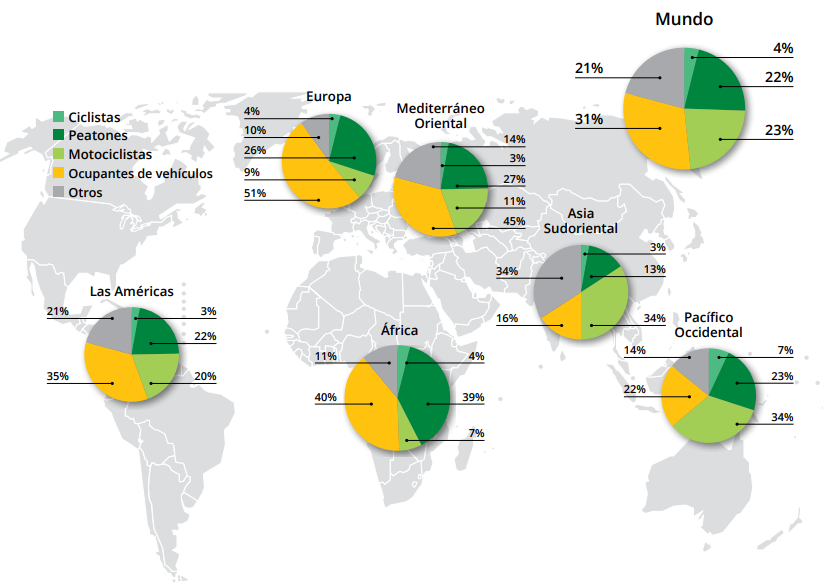
\includegraphics[width=0.9\textwidth, fbox]{imagenes/Cap1/oms1}
  \caption{Muertes por accidentes de tránsito por regi\'{o}n en función del tipo de usuario (2013), OMS}
  \label{fig:oms}  
  \end{center}
\end{figure}

Por otro lado seg\'{u}n la Unidad Operativa de Tr\'{a}nsito de Cochabamba los accidentes registrados en 2017 provocaron la muerte de 200 personas y dejaron aproximadamente 2200 heridos.
	
\vspace{5mm} %5mm vertical space

En la figura \ref{fig:arbol} se muestra las causas por las cuales se ocasiona un accidente de tr\'{a}nsito, se puede observar que gran parte de \'{e}stas se deben al factor humano sin embargo hay otras que conllevan factores medio-ambientales y mec\'{a}nicos, por lo que se hace imposible evitar completamente los mismos. 

\vspace{5mm} %5mm vertical space

Es por ello que se hace necesario el contar con mecanismos para prevenir y/o actuar de forma oportuna ante posibles accidentes de tr\'{a}nsito, motivo por el cual el presente trabajo se centra en estudiar los comportamientos de conducci\'{o}n, para as\'{i} generar alertas al encontrar un comportamiento an\'{o}malo en el manejo, de manera que se pueda evitar o en todo caso minimizar los efectos del mismo.

\begin{figure}[h!]
  \begin{center}	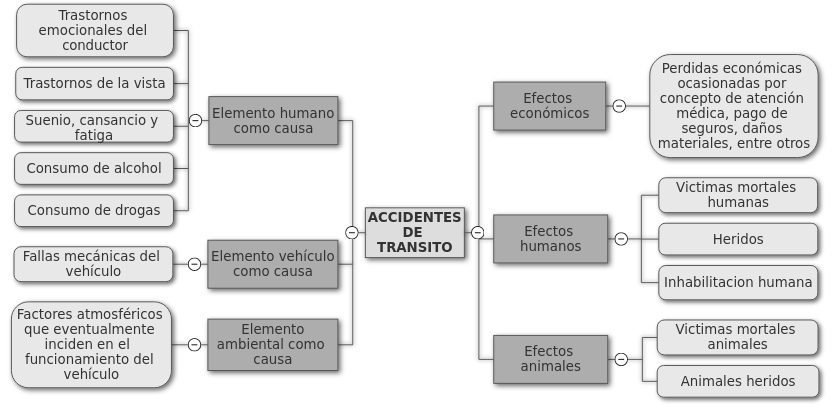
\includegraphics[width=1.0\textwidth, fbox]{imagenes/Cap1/arbol_p}
  \caption{\'{A}rbol de problemas}
  \label{fig:arbol}
  \end{center}
\end{figure}


\section{Objetivo general}

El objetivo general del presente trabajo es desarrollar un mecanismo de detecci\'{o}n de anomal\'{i}as de conducción, mediante el uso de un dispositivo móvil y algoritmos de Aprendizaje Automático, con el fin de alertar de forma oportuna el hallazgo de un patrón anómalo en el manejo, tal como cansancio, ebriedad, o problemas de salud, ej, epilepsia.

\section{Objetivos específicos}
\begin{itemize}

\item Capturar los parámetros de manejo de un conductor mediante el uso de sensores de un dispositivo móvil.
\item Escalar los parámetros de manejo mediante técnicas de pre-procesamiento de datos.
\item Generar un modelo de aprendizaje automático que se ajuste a un comportamiento normal de manejo.
\item Definir un método de detección de anomalías para generar una alerta de conducción anormal.
\item Evaluar el método de detección de anomalías con nuevas muestras.

\end{itemize}


\section{Justificación}

Los accidentes de tránsito cobran un número inaceptable de víctimas cada a\~{n}o, especialmente en las regiones m\'{a}s pobres del mundo. Esto se debe a diversos aspectos, pero el principal recae en el bajo nivel de conciencia ciudadana que existe, lo que conlleva a que muchas personas conduzcan bajo los efectos del alcohol, con exceso de velocidad, manipulando sus dispositivos m\'{o}viles, entre otros. Por ello este trabajo busca establecer patrones de comportamientos de conducci\'{o}n mediante el uso de un dispositivo m\'{o}vil y t\'{e}cnicas de Aprendizaje Autom\'{a}tico, de manera que se logre realizar una detecci\'{o}n de anomal\'{i}as de conducci\'{o}n oportuna.

\subsection{Justificaci\'{o}n pr\'{a}ctica}

Detectar anomal\'{i}as de conducci\'{o}n permite generar una alerta oportuna a las autoridades o a los agentes para que logren corregir sus conductas de conducci\'{o}n de forma r\'{a}pida. De esta manera se podr\'{a} evitar accidentes de tr\'{a}nsito o minimizar los efectos del mismo, permitiendo as\'{i} reducir la cantidad de da\~{n}os, tanto materiales como personales.

\subsection{Justificaci\'{o}n metodol\'{o}gica}

El estudio realizado en el desarrollo del presente trabajo de investigaci\'{o}n permite resaltar la eficiencia de las t\'{e}cnicas de Inteligencia Artificial en la detecci\'{o}n de anomal\'{i}as.

\section{L\'{i}mites y alcances}

Debido a que la realizaci\'{o}n de pruebas de campo para \'{e}sta investigaci\'{o}n es bastante peligrosa, se limit\'{o} los ejemplos de conducci\'{o}n an\'{o}mala a:

\begin{itemize}
\item Frenos en seco.
\item Giros hacia la derecha e izquierda a alta velocidad.
\item Giros en zig zag bruscos.
\end{itemize}

\vspace{5mm} %5mm vertical space

Siendo as\'{i} los experimentos y pruebas se realizaron s\'{o}lo sobre un peque\~{n}o conjunto de ejemplos an\'{o}malos, por lo tanto no se espera que el modelo de detecci\'{o}n propuesto funcione de manera correcta sobre aquellos ejemplos que no fueron considerados.

\section{M\'{e}todo de investigaci\'{o}n}

El presente estudio se realiz\'{o} con un enfoque experimental, teniendo como hip\'{o}tesis la siguiente:


\begin{center}
\textit{\large{¿Es posible detectar anomal\'{i}as de conducci\'{o}n mediante el uso de un dispositivo móvil y algoritmos de Aprendizaje Autom\'{a}tico?}}
\end{center}


% Chapter 2

\chapter{\uppercase{FUNDAMENTALS OF THE DETECTION OF ANOMALIES}}

\label{Capitulo 2}

This chapter discusses necessary concepts that are needed to understand the detection of anomalies, as well as different projects and investigations carried out in field of the detection of driving anomalies to date.
%En este cap\'{i}tulo se aborda los conceptos necesarios que se necesita para comprender la detecci\'{o}n de anomal\'{i}as, as\'{i} tambi\'{e}n se expone los diferentes proyectos e investigaciones realizados en el campo de la detecci\'{o}n de anomal\'{i}as de conducci\'{o}n hasta la fecha.

\section{Anomaly detection}

To understand what anomaly detection implies, it is necessary to assimilate what an anomaly is, and in what ways these can occur. Therefore, it can be said that anomalies, or outliers, are patterns in the data that do not fit a well-defined notion of normal behavior.
%Para comprender lo que implica la detecci\'{o}n de anomal\'{i}as, es necesario asimilar lo que \'{e}s una anomal\'{i}a, y de qu\'{e} maneras \'{e}stas pueden presentarse. Por lo tanto, se puede decir que las \textbf{anomalías}, o valores at\'{i}picos, son patrones en los datos que no se ajustan a una noción bien definida de un comportamiento normal.

\vspace{5mm} %5mm vertical space

Anomalies can be classified into one of the following three categories:
%Las anomal\'{i}as pueden ser clasificadas dentro de una de las tres siguientes categor\'{i}as:

\begin{enumerate}[1.]

\item \textbf{Point anomalies: }Point anomalies are simply unique and anomalous instances within a larger data set, that is, they are separated from the rest of the data. For example, in Figure \ref{fig:anom_2D}, points $o_1$, $o_2$ and region $O_3$ are outside the limits of normal regions ($N_1$ and $N_2$), and therefore are point anomalies because they are different from the normal data set.

%\item \textbf{Anomal\'{i}as de punto: }Las anomalías de punto son simplemente instancias únicas y anómalas dentro de un conjunto de datos más grande, es decir, \'{e}stas se encuentran separadas del resto de los datos. Por ejemplo, en la Figura \ref{fig:anom_2D}, los puntos $o_1$, $o_2$ y la regi\'{o}n $O_3$ se encuentran fuera de los l\'{i}mites de las regiones normales ($N_1$ y $N_2$), y por lo tanto son anomal\'{i}as puntuales debido a que son diferentes al conjunto de datos normales.

\begin{figure}[h!]
  \begin{center}	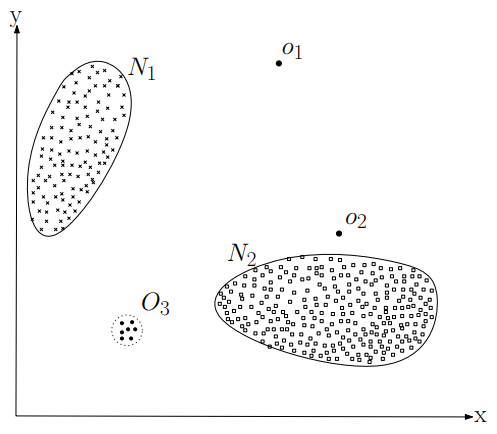
\includegraphics[width=0.45\textwidth,frame]{imagenes/Cap2/anom_2D}
  \caption{Example of point anomalies in a 2-dimensional data set \protect\cite{Reference66}.}
  \label{fig:anom_2D}
  \end{center}
\end{figure}

\vspace{5mm} %5mm vertical space

This type of anomaly is considered the simplest and is the focus of most research focused on anomaly detection.
%Este tipo de anomal\'{i}a se considera la m\'{a}s simple y es el foco de la mayor\'{i}a de las investigaciones enfocadas en la detecci\'{o}n de valores at\'{i}picos.

\item \textbf{Contextual (or conditional) anomalies: }These are points that are only considered anomalous in a specific context. The notion of this context is induced by the structure in the data set and must be specified as part of the problem formulation.
%\item \textbf{Anomal\'{i}as contextuales (o condicionales): }Estos son puntos que s\'{o}lo se consideran anómalos en un contexto espec\'{i}fico. La noci\'{o}n de este contexto es inducida por la estructura en el conjunto de datos y debe especificarse como parte de la formulaci\'{o}n del problema.

\vspace{5mm} %5mm vertical space

These types of anomalies have been explored more frequently in time series and spatial data. Figure \ref{fig:anom_contx} shows an example of a time series of the monthly temperature of an area in the last 5 years, it should be taken into account that the temperature at time $t_1$ is the same as at time $t_2$, but occurs in a different context , therefore $t_2$ is considered an anomaly.
%Este tipo de anomal\'{i}as se han explorado con mayor frecuencia en los datos de series de tiempo y datos espaciales. La figura \ref{fig:anom_contx} muestra un ejemplo de serie temporal de la temperatura mensual de un \'{a}rea en los \'{u}ltimos 5 a\~{n}os, se debe tener en cuenta que la temperatura en el tiempo $t_1$ es la misma que en el tiempo $t_2$, pero se produce en un contexto diferente, por lo tanto $t_2$ es considerada una anomal\'{i}a.

\begin{figure}[h!]
  \begin{center}	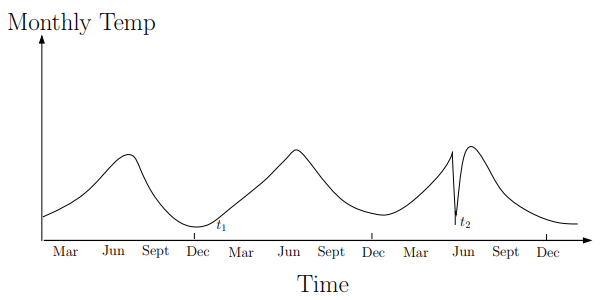
\includegraphics[width=0.6\textwidth,frame]{imagenes/Cap2/anom_contx}
  \caption{Contextual anomaly $t_2$ in a temperature time serie \protect\cite{Reference66}.}
  \label{fig:anom_contx}
  \end{center}
\end{figure}

\item \textbf{Collective anomalies: } If a collection of related data instances is anomalous with respect to the entire data set, it is called a collective anomaly. The instances of individual data in a collective anomaly may not be anomalies by themselves, but their joint appearance as a collection is anomalous.
%\item \textbf{Anomal\'{i}as colectivas: } Si una colección de instancias de datos relacionadas es anómala con respecto a todo el conjunto de datos, se denomina anomalía colectiva.  Las instancias de datos individuales en una anomalía colectiva pueden no ser anomalías por sí mismas, pero su aparición conjunta como una colección es anómala.

\vspace{5mm} %5mm vertical space

Figure \ref{fig:anom_col} illustrates an example showing a human electrocardiogram output, it can be noted that the region highlighted in red denotes an anomaly because there is the same low value for an abnormally long time (corresponding to a premature atrial contraction). It should be taken into account that this low value by itself is not considered an anomaly.
%La figura \ref{fig:anom_col} ilustra un ejemplo que muestra una salida de electrocardiograma humano, se puede notar que la región resaltada en rojo denota una anomalía porque existe el mismo valor bajo durante un tiempo anormalmente prolongado (que corresponde a una Contracción prematura auricular). Se debe tener en cuenta que ese valor bajo por sí mismo no es considerada una anomalía.

\begin{figure}[h!]
  \begin{center}	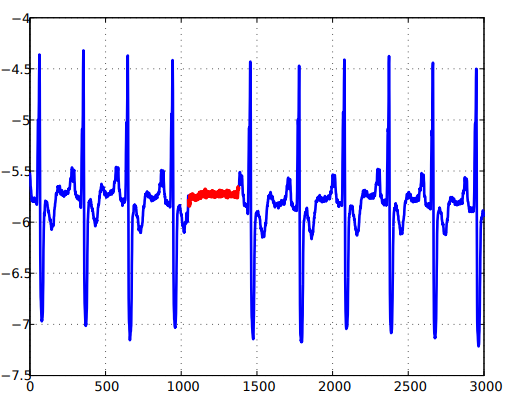
\includegraphics[width=0.45\textwidth,frame]{imagenes/Cap2/anom_col}
  \caption{Collective anomaly corresponding to premature atrial contraction in a human electrocardiogram \protect\cite{Reference66}.}
  \label{fig:anom_col}
  \end{center}
\end{figure}

\end{enumerate}

In relation to the above, it can be defined as detection of anomalies, or outliers, to the identification of data points, elements, observations or events that do not fit the expected pattern of a particular group.
%En relaci\'{o}n a lo expuesto previamente se puede definir como \textbf{detecci\'{o}n de anomal\'{i}as}, \'{o} \textbf{valores at\'{i}picos}, a la identificación de puntos de datos, elementos, observaciones o eventos que no se ajustan al patrón esperado de un grupo determinado. 

\vspace{5mm} %5mm vertical space

Anomaly detection is used in different application domains, for example: image processing, card fraud detection, network intrusion detection systems, etc.
%La detecci\'{o}n de anomal\'{i}as, se usa en distintos dominios de aplicaciones, por ejemplo: procesamiento de im\'{a}genes, detecci\'{o}n de fraudes de tarjeta, sistemas de detecci\'{o}n de intrusi\'{o}n de red, \'{e}tcetera.

\section{Challenges in anomaly detection}

On an abstract level, anomaly detection may seem like a simple task. However, it can be a very challenging task. Below are some of these challenges.
%En un nivel abstracto, la detecci\'{o}n de anomal\'{i}as puede parecer una tarea simple. Sin embargo puede llegar a ser una tarea muy desafiante. A continuaci\'{o}n se presenta algunos de estos desaf\'{i}os.

\begin{itemize}
\item The definition of normal regions is quite difficult. In many cases, the boundaries between anomalies and normal data are not accurate. Therefore, normal observations could be considered anomalies and vice versa.
%\item La definici\'{o}n de regiones normales es bastante dif\'{i}cil. En muchos casos, los l\'{i}mites entre las anomal\'{i}as y los datos normales no son precisos. Por lo tanto, las observaciones normales podr\'{i}an considerarse anomal\'{i}as y viceversa.

\item Therefore, normal observations could be considered anomalies and vice versa.
%\item Lo que se considera normal hoy en d\'{i}a, puede no ser normal en el futuro.

\item Most of the time the approaches for detecting anomalies in a specific field cannot be used in another field.
%\item La mayor parte de las veces los enfoques para la detecci\'{o}n de anomal\'{i}as en un campo en espec\'{i}fico no se pueden utilizar en otro campo.

\item The low availability of positive samples (anomalies) for training and validation of anomaly detection model.
%\item La poca disponibilidad de ejemplos positivos (anomal\'{i}as) para el entrenamiento y validaci\'{o}n del modelo de detecci\'{o}n de anomal\'{i}as.

\end{itemize}

\subsection{Anomaly detection approaches}

The approaches that can be used for this purpose are classified into following categories:
%Los enfoques que se pueden usar para este prop\'{o}sito se clasifican en las siguientes categor\'{i}as:

\subsubsection{Supervised anomaly detection}

The use of supervised learning techniques requires the availability of a set of labeled training data, for both normal and anomalous classes. The main focus is to build a predictive model for normal classes vs. anomalies, then take any instance of unseen data, compare with model and determine to which class it belongs.
%El uso de t\'{e}cnicas de aprendizaje supervisado requiere la disponibilidad de un conjunto de datos de entrenamiento etiquetados, tanto para clases normales como an\'{o}malas. El enfoque principal es construir un modelo predictivo para clases normales vs. anomal\'{i}as, posteriormente tomar cualquier instancia de datos no visto, comparar con el modelo y determinar a que clase pertenece.

\vspace{5mm} %5mm vertical space

There are two main drawbacks that arise with the use of this technique.
%Existen dos principales inconvenientes que surgen con el uso de \'{e}sta t\'{e}cnica.

\begin{itemize}

\item The number of anomalous instances is much lower than that of the normal instances, which creates an imbalance of class distribution during training.
%\item La cantidad de instancias an\'{o}malas es muy inferior a la de las instancias normales, lo que genera un desequilibrio de distribuci\'{o}n de clases durante el entrenamiento.
\item Obtaining accurate and representative labels, particularly for anomaly class, is a challenge.
%\item La obtenci\'{o}n de etiquetas precisas y representativas, en particular para la clase de anomal\'{i}a, es un desaf\'{i}o.
\end{itemize}

\subsubsection{Semi-supervised anomaly detection}

These techniques require a training set with labeled instances, but only for the normal class, this makes its use more applicable than the supervised techniques, since no labels are required for the anomaly class.
%Estas t\'{e}cnicas requieren un conjunto de entrenamiento con instancias etiquetadas, pero solo para la clase normal, esto hace que su uso sea m\'{a}s aplicable que las t\'{e}cnicas supervisadas, ya que no se requiere etiquetas para la clase anomal\'{i}a.

\vspace{5mm} %5mm vertical space

The typical approach used in these techniques is to build a model for the class corresponding to normal behavior, and use model to identify anomalies in the test data.
%El enfoque típico usado en \'{e}stas técnicas es construir un modelo para la clase correspondiente al comportamiento normal, y usar el modelo para identificar anomalías en los datos de prueba.

\subsubsection{Unsupervised anomaly detection}

Techniques that operate in an unsupervised manner do not require training data, which is why they are the most widely used. These techniques assume that normal instances are much more frequent than anomalies in test data, in case this assumption is not true, such techniques suffer from a high rate of false alarms.
%Las t\'{e}cnicas que operan de manera no supervisada no requieren datos de entrenamiento, raz\'{o}n por la cual son las m\'{a}s ampliamente utilizadas. Estas t\'{e}cnicas suponen que las instancias normales son mucho m\'{a}s frecuentes que  las anomal\'{i}as en los datos de prueba, en caso de que esta suposici\'{o}n no sea cierta, tales t\'{e}cnicas sufren de una alta tasa de falsas alarmas.

\section{Related work}

The identification of abnormal driving behaviors is an indispensable part of improving driving safety, however, as previously described, this is not a simple task. In recent years, several techniques have been proposed to detect driving behaviors. This section is dedicated to review them.
%La identificación de comportamientos de conducción anormal es una parte indispensable para mejorar la seguridad de conducción, sin embargo, como se describi\'{o} previamente, \'{e}sta no es una tarea sencilla. En los últimos años, se han propuesto varias técnicas para detectar conductas de conducci\'{o}n. Esta secci\'{o}n esta dedicada al repaso de las mismas.

\vspace{5mm} %5mm vertical space

\shortciteA{Reference20}, propose a combined system that consists of two modules: one to detect the type of vehicle of users and the other to detect events of instant driving, regardless of the orientation and position of smartphones, this system It achieves an average accuracy of 98.33\% in detection of vehicles's type (car, motorcycle, bicycle, among others) and an average accuracy of 98.95\% in recognition of motorcyclist driving events when using Random Forest as a classifier.
%\shortciteA{Reference20}, proponen un sistema combinado que se compone de dos módulos: uno para detectar el tipo de vehículo de los usuarios y el otro para detectar los eventos de conducción instantánea, independientemente de la orientación y la posición de los teléfonos inteligentes, \'{e}ste sistema logra una precisión promedio del 98.33\% en la detección del tipo del vehículo (autom\'{o}vil, motocicleta, bicicleta, entre otros) y una precisión promedio de 98.95\% en el reconocimiento de los eventos de conducción de los motociclistas al usar Random Forest como clasificador.

\vspace{5mm} %5mm vertical space

On the other hand \shortciteA{Reference21} present a quantitative evaluation of 4 Machine Learning algorithms (Bayesian Network BN, Artificial Neural Network ANN, Random Forest RF and Support Vector Machine SVM) with different configurations, applied in the detection of 7 types of driving events, between events normal and aggressive, using data collected from 4 Android smartphone sensors (accelerometer, linear acceleration, magnetometer and gyroscope); resulting in the gyroscope and accelerometer being the best sensors to detect driving events and that Random Forest (RF) is by far the best-performing Machine Learning Algorithm, followed by the simplest form of ANN the Multi Layer Perceptron ( MLP).
%Por otra parte \shortciteA{Reference21} presentan una evaluación cuantitativa de 4 algoritmos de Aprendizaje Autom\'{a}tico ( Bayesian Network BN, Artificial Neural Network ANN, Random Forest RF y Support Vector Machine SVM) con diferentes configuraciones, aplicadas en la detección de 7 tipos de eventos de conducción, entre eventos normales y agresivos, utilizando datos recopilados de 4 sensores de teléfonos inteligentes Android (acelerómetro, aceleración lineal, magnetómetro y giroscopio); dando como resultado que el giroscopio y el acelerómetro son los mejores sensores para detectar eventos de conducción y que Random Forest (RF) es por lejos el Algoritmo de Aprendizaje Autom\'{a}tico de mejor rendimiento, seguido de la forma m\'{a}s simple de ANN el Multi Layer Perceptron (MLP).

\vspace{5mm} %5mm vertical space

\citeA{Reference23} propose the MIROAD system which shows that Dynamic Time Warping (DTW) is a valid algorithm to detect potentially aggressive driving maneuvers, where almost all aggressive events (97\%) were correctly identified, using the set of T sensors (accelerometer, gyroscope and tone of voice). Likewise, in the work of Kridalukmana, Yan-Lu, and Naderpour (2017), a system focused on developing driver awareness through notifications in critical situations that can trigger unsafe driving maneuvers is proposed, using a model to detect dangerous situations based on Object-Oriented Bayesian Network (OOBN).
%\citeA{Reference23} proponen el sistema MIROAD el cual muestra que el Dynamic Time Warping (DTW) es un algoritmo válido para detectar maniobras de conducción potencialmente agresivas, donde casi todos los eventos agresivos (97\%) se identificaron correctamente, utilizando el conjunto de sensores T (aceler\'{o}metro, giroscopio y el tono de voz). As\'{i} tambi\'{e}n en el trabajo de \citeA{Reference24} se propone un sistema enfocado a desarrollar la conciencia del conductor mediante notificaciones en situaciones críticas que pueden desencadenar maniobras de conducci\'{o}n inseguras, mediante un modelo para detectar situaciones peligrosas basadas en Object-Oriented Bayesian Network (OOBN).

\vspace{5mm} %5mm vertical space

As well as the works presented previously there is a large number of works (\citeNP{Reference25}; \citeNP{Reference26}; \citeNP{Reference27}; \citeNP{Reference28}; \citeNP{Reference29}) that use smart phone sensors (accelerometer and gyroscope) for aggressive driving detection, due of advantage of not buying or installing any device and besides being highly portable, however it depends a lot on the performance of GPS receiver and is not applicable in areas not available for GPS.
%As\'{i} como los trabajos presentados previamente existe gran cantidad de trabajos (\citeNP{Reference25}; \citeNP{Reference26}; \citeNP{Reference27}; \citeNP{Reference28}; \citeNP{Reference29}) que usan los sensores de los tel\'{e}fonos inteligentes (aceler\'{o}metro y giroscopio) para la detecci\'{o}n de conducci\'{o}n agresiva, esto debido a que se tiene la ventaja de no comprar ni instalar ning\'{u}n dispositivo y adem\'{a}s de ser altamente port\'{a}til, sin embargo se depende bastante del rendimiento del receptor GPS y no es aplicable en \'{a}reas no disponibles para GPS.

\vspace{5mm} %5mm vertical space

There are also other approaches to detection of aggressive driving of a driver, for instance in the work of \citeA{Reference22}, a method based on Convolutional Neural Network (CNN) is proposed) to detect the emotion of aggressive driving, by using a driver's facial images obtained with a NIR light camera and a thermal camera.
%Existen adem\'{a}s otros enfoques para la detecci\'{o}n de conducci\'{o}n agresiva de un conductor, por ejemplo en el trabajo de \citeA{Reference22} se propone un método basado en Convolutional Neural Network (CNN) para detectar la emoción de conducción agresiva, mediante la utilizaci\'{o}n de imágenes faciales de un conductor obtenidas con una cámara de luz NIR y una cámara térmica.

\section{Focus on the problem}

It is clear that this topic was extensively researched and that it has a wide variety of solution proposals, however most of these are based on detection by supervised learning techniques, which presents the great disadvantage of requiring data labeled to generate the model detection; In addition, much of related work proposes generalized models for detection and not specific models for each agent, which is crucial because each agent has individual driving behaviors and different conditions driving, that is, the driving of an agent that circulates through paved avenues will be different from driving of an agent that circulates through cobbled streets or driving of an agent that circulates through avenues or busy streets will be different from that of the agents that circulate through relatively decongested streets.
%Es evidente que \'{e}ste tema fue ampliamente investigado y que tiene una gran variedad de propuestas de soluci\'{o}n, sin embargo la mayor\'{i}a de estas se basan en la detecci\'{o}n mediante t\'{e}cnicas de aprendizaje supervisado, lo cual presenta la gran desventaja de requerir datos etiquetados para generar el modelo de detecci\'{o}n; adem\'{a}s gran parte de los trabajos relacionados proponen modelos generalizados para la detecci\'{o}n y no as\'{i} modelos espec\'{i}ficos por cada agente, lo cual es crucial debido a que cada agente presenta conductas individuales de conducci\'{o}n y conducen en condiciones distintas, es decir, la conducci\'{o}n de un agente que circula por avenidas pavimentadas ser\'{a} distinta a la conducci\'{o}n de un agente que circula por calles empedradas o la conducci\'{o}n de un agente que circula por avenidas o calles concurridas ser\'{a} distinta a de los agentes que circulen por calles relativamente descongestionadas.

\vspace{5mm} %5mm vertical space

The proposal made in this work is intended to provide a prototype of a tool that helps analyze the sequences of motion sensors of a mobile device and allows detecting anomalies from information obtained from this analysis.
%Con la propuesta que se hace en este trabajo se pretende brindar un prototipo de una herramienta que ayude a analizar las secuencias de los sensores de movimiento de un dispositivo m\'{o}vil y permita detectar anomalías a partir de la información obtenida de este análisis. 

\vspace{5mm} %5mm vertical space

To achieve this goal, the data set of motion sensors of a smartphone is captured, using a mobile application, then data is divided and prepared with data pre-processing techniques. Once these phases are completed, a model is trained with the training set and validated with the development set. Finally, an optimal model and a technique are chosen to classify outliers, in order to cover a full range of normal behaviors and exclude anomalies as accurately as possible. This method can best be seen in Figure \ref{fig:modeloAnomalias}.
%Para lograr este objetivo, se captura el conjunto de datos de los sensores de movimiento de un tel\'{e}fono inteligente, mediante una aplicaci\'{o}n m\'{o}vil, posteriormente se divide y prepara los datos con t\'{e}cnicas de pre-procesamiento de datos. Una vez terminadas estas fases se entrena un modelo con el conjunto de entrenamiento y se valida con el conjunto de desarrollo. Finalmente se elige un modelo \'{o}ptimo y una t\'{e}cnica para clasificar los valores at\'{i}picos, con el objetivo de cubrir un rango completo de los comportamientos normales y excluir con la mayor precisi\'{o}n posible las anomal\'{i}as. Este m\'{e}todo se puede apreciar mejor en la Figura \ref{fig:modeloAnomalias}.

\begin{figure}[h!]
  \begin{center}	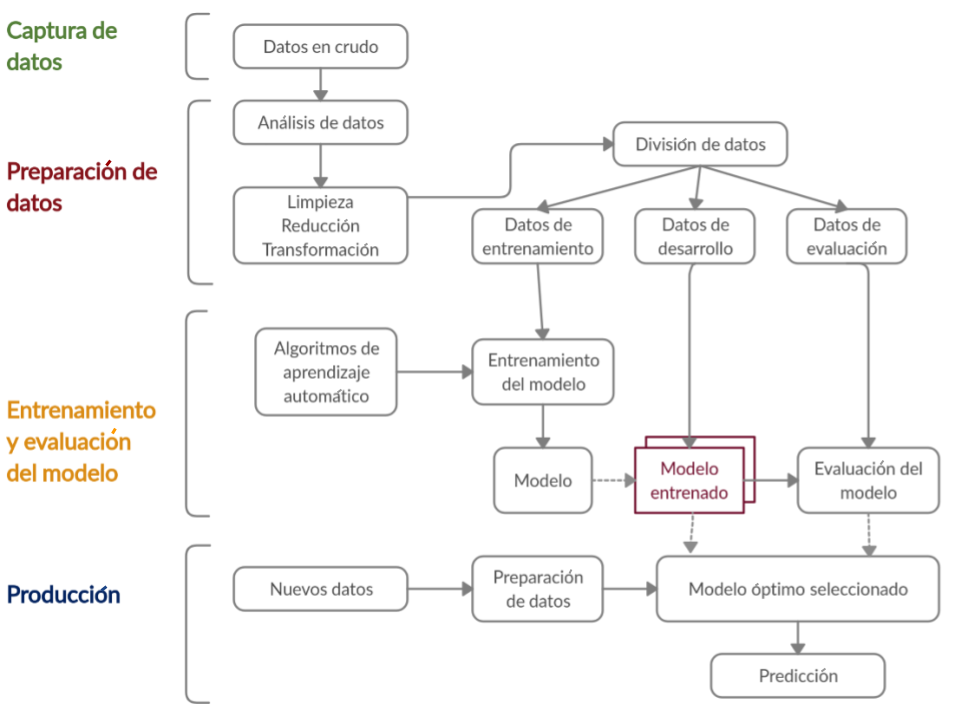
\includegraphics[width=0.90\textwidth,frame]{imagenes/Cap2/metodo1}
  \caption{Proposed anomaly detection method (Own elaboration).}
  \label{fig:modeloAnomalias}
  \end{center}
\end{figure}
%https://app.creately.com/diagram/XJJlVcfuoWy/view

%\section{Resumen del cap\'{i}tulo}

%De acuerdo a los conceptos presentados acerca de la detecci\'{o}n de anomal\'{i}as, los desaf\'{i}os  que presenta la detecci\'{o}n de las mismas y los trabajos de investigaci\'{o}n realizados en este campo hasta la fecha, se propone un m\'{e}todo de detecci\'{o}n de anomal\'{i}as de conducci\'{o}n mediante el uso de t\'{e}cnicas de Aprendizaje Autom\'{a}tico y el uso de un dispositivo m\'{o}vil, los mismos ser\'{a}n tratados en profundidad en los siguientes cap\'{i}tulos.
\chapter{\uppercase{Machine Learning for Anomaly detection}}
\label{Capitulo 3}

The term Machine Learning refers to the automatic detection of significant patterns within a data set \cite{Reference32}. In recent decades it has become a common tool in almost any task that requires the extraction of information from a large amount of data, which is why it has become one of the fastest growing areas of information technology.
%El t\'{e}rmino Aprendizaje Autom\'{a}tico se refiere a la detecci\'{o}n autom\'{a}tica de patrones significativos dentro de un conjunto de datos \cite{Reference32}. En las \'{u}ltimas d\'{e}cadas se ha convertido en una herramienta com\'{u}n en casi cualquier tarea que requiera la extracci\'{o}n de informaci\'{o}n de gran cantidad de datos, por lo cual se ha convertido en una de las \'{a}reas de m\'{a}s r\'{a}pido crecimiento de la inform\'{a}tica.

\vspace{5mm} %5mm vertical space

Although Machine Learning can solve some problems that are solved with traditional algorithms, it has overcome these problems such as image recognition, voice, language, writing, games, robotics, data analysis, time series analysis, etc. From this perspective, it is expected that through the application of Machine Learning a model can be generated that fits to a normal behavior expected for the agent.
%Si bien el Aprendizaje Autom\'{a}tico puede resolver algunos problemas que son resueltos con algoritmos tradicionales, ha superado a \'{e}stos en problemas tales como el reconocimiento de im\'{a}genes, voz, lenguaje, escritura, juegos, rob\'{o}tica, an\'{a}lisis de datos, an\'{a}lisis de series de tiempo, etc. Desde esta perspectiva, se espera que mediante la aplicaci\'{o}n del Aprendizaje Autom\'{a}tico se pueda generar un modelo que se ajuste a un comportamiento normal esperado para el agente.

\vspace{5mm} %5mm vertical space

Therefore, this chapter details the theoretical bases necessary to address the development of the method for driving anomaly detection. First, the different learning paradigms that exist and the different model approaches are described, then, a description of the functioning of neural networks is made and the different types of networks are shown, as well as different techniques of anomaly detection that exist and finally shows different evaluation metrics presented by machine learning models.
%Por lo tanto en este cap\'{i}tulo se detalla las bases te\'{o}ricas necesarias para abordar el desarrollo del m\'{e}todo de detecci\'{o}n de anomal\'{i}as de conducci\'{o}n. En primer lugar, se decribe los diferentes paradigmas de aprendizaje que existen y los diferentes enfoques de modelos, luego, se realiza una descripci\'{o}n del funcionamiento de las redes neuronales y se muestra los diferentes tipos de redes, as\'{i} como tambi\'{e}n se presenta las diferentes t\'{e}cnicas de detecci\'{o}n de anomal\'{i}as que hay y por \'{u}timo se muestra las diferentes m\'{e}tricas de evaluaci\'{o}n que presentan los modelos de aprendizaje autom\'{a}tico. 

\section{Supervised Learning, Unsupervised Learning and Semi Supervised Learning}
\label{section|aprendizaje}

There are several ways to classify learning paradigms that exist, however in this work only supervised, unsupervised and semi-supervised will be treated.
%Existen diversas formas de clasificar los paradigmas de aprendizaje que existen, sin embargo en el presente trabajo s\'{o}lo se tratar\'{a}n el supervisado, el no supervisado y el semi-supervisado.

\subsection{Supervised Learning}

\textbf{Supervised Learning} is one that has input variables (X) and an output variable (Y), this type of learning uses an algorithm to learn the mapping function from input to output.
%El \textbf{Aprendizaje Supervisado} es aquel que cuenta con variables de entrada (X) y una variable de salida (Y), este tipo de aprendizaje utiliza un algoritmo para aprender la funci\'{o}n de mapeo desde la entrada hasta la salida.

\begin{equation}
Y = f(X)
\end{equation}

The objective of this type of learning is to approximate the mapping function so that when you have new input data (X) you can predict the output variables (Y) for that data.
%El objetivo de este tipo de aprendizaje es aproximar la funci\'{o}n de mapeo de tal forma que cuando tenga datos de entrada nuevos (X) pueda predecir las variables de salida (Y) para esos datos. 

\vspace{5mm} %5mm vertical space

This type of learning addresses two types of problems: classification and regression. Classification problems are those where the output variable is a category, such as: ''Red'', ''Blue'', or ''Healthy'', ''Sick'', on the other hand in Regression problems the output variable is a real value, such as: ''price'' or ''height''. Some of the most common types of problems built on classification and regression include recommendation and prediction of time series.
%Este tipo de aprendizaje aborda dos tipos de problemas: clasificaci\'{o}n y regresi\'{o}n. Los problemas de \textbf{Clasificaci\'{o}n} son aquellos donde la variable de salida es una categor\'{i}a, como por ejemplo: ''Rojo'', ''Azul'', o ''Sano'', ''Enfermo'', por otra parte en los problemas de \textbf{Regresi\'{o}n} la variable de salida es un valor real, tal como: ''precio'' o ''altura''. Algunos de los tipos de problemas m\'{a}s comunes construidos sobre la clasificaci\'{o}n y la regresi\'{o}n incluyen la recomendaci\'{o}n y la predicci\'{o}n de series temporales.

\subsection{Unsupervised Learning}

On the other hand, Non-Supervised Learning is one where there is only input data (X) and there are no corresponding output variables, its main objective is to model the structure or underlying distribution in  data to learn more about them.
%Por otro lado el \textbf{Aprendizaje no Supervisado} es aquel donde s\'{o}lo se cuenta con datos de entrada (X) y no hay variables de salida correspondientes, su objetivo principal consiste en modelar la estructura o distribuci\'{o}n subyacente en los datos para aprender m\'{a}s acerca de los mismos.

\vspace{5mm} %5mm vertical space

As for learning problems without supervision, they can be grouped into two: grouping and association. \textbf{Grouping} is one where you want to discover the groupings inherent in data set, such as grouping customers by purchasing behavior. On the other hand,  \textbf{Association} is one that wishes to discover rules that describe large portions of its data, for example, people who buy X also tend to buy Y. Some of the most popular unsupervised learning algorithms are: Kmeans (for clustering problems) and Apriori algorithm (for learning problems of association rules).
%En cuanto a los problemas del Aprendizaje sin supervisi\'{o}n, pueden ser agrupados en dos: agrupamiento y asociaci\'{o}n. El \textbf{Agrupamiento} es aquel donde se desea descubrir las agrupaciones inherentes en el conjunto de datos, como por ejemplo agrupar clientes por comportamiento de compra. Por otra parte la \textbf{Asociaci\'{o}n} es aquella que desea descubrir reglas que describen grandes porciones de sus datos, por ejemplo las personas que compran X tambi\'{e}n tienden a comprar Y. Algunos de los algoritmos de aprendizaje sin supervisi\'{o}n m\'{a}s populares son: K-means (para problemas de agrupamiento) y algoritmo Apriori (para problemas de aprendizaje de reglas de asociaci\'{o}n).

\subsection{Semi Supervised Learning}

Finally, there is Semi-supervised Learning, which covers those problems where there is a large amount of input data (X) and only some of data is labeled (Y). These types of problems are between supervised and unsupervised learning, it is also important to point out that many of Machine Learning's problems in the real world are in this area, this is because it is expensive or it may take a long time to label the data set, while unlabeled data is cheap, in addition to being easy to collect and store. These types of problems can use a combination of supervised and unsupervised techniques to be solved.
%Por \'{u}ltimo se encuentra el \textbf{Aprendizaje Semi-supervisado}, el cual abarca aquellos problemas donde se tiene gran cantidad de datos de entrada (X) y s\'{o}lo algunos de los datos est\'{a}n etiquetados (Y). Este tipo de problemas se encuentran entre el aprendizaje supervisado y el no supervisado, adem\'{a}s es importante se\~{n}alar que muchos de los problemas de Aprendizaje Autom\'{a}tico en el mundo real se encuentran en esta \'{a}rea, esto debido a que resulta costoso o puede requerir mucho tiempo etiquetar el conjunto de datos, mientras que los datos no etiquetados son baratos, adem\'{a}s de ser f\'{a}ciles de recolectar y almacenar. Este tipo de problemas pueden usar una combinaci\'{o}n de t\'{e}cnicas supervisadas y no supervisadas para ser resueltos.

\vspace{5mm} %5mm vertical space

Since Supervised Learning methods require a large amount of labeled training data, it is important to clarify that the collection of negative samples (abnormal driving) is difficult and risky for this particular study; In addition, the supervised approach has a potential limitation, which is: the detection of new atypical patterns, this because the resulting model is only trained to recognize a limited set of anomalous patterns, so at the time a new one is presented pattern this model will be unable to recognize it.
%Dado que los m\'{e}todos de Aprendizaje Supervisado requieren una gran cantidad de datos de entrenamiento etiquetados, es importante aclarar que la recolecci\'{o}n de muestras negativas (conducci\'{o}n an\'{o}mala) es d\'{i}ficil y riesgosa para este estudio en particular; adem\'{a}s el enfoque supervisado presenta una limitaci\'{o}n potencial, la cual es: la detecci\'{o}n de nuevos patrones at\'{i}picos, esto debido a que el modelo resultante s\'{o}lo esta entrenado para reconocer un conjunto limitado de patrones an\'{o}malos, por lo cual al momento en que se presente un nuevo patr\'{o}n este modelo ser\'{a} incapaz de reconocerlo.

\vspace{5mm} %5mm vertical space

On the other hand, unsupervised approach has advantage of not requiring tagged information, however it often suffers from high false alarm rates and low detection rates \cite{Reference33}.
%Por otra parte el enfoque sin supervisi\'{o}n tiene la ventaja de no requerir informaci\'{o}n etiquetada, sin embargo a menudo sufre altas tasas de falsas alarmas y bajas tasas de detecci\'{o}n \cite{Reference33}. 

\vspace{5mm} %5mm vertical space

In many applications, including the one of present study, normal samples are easy to obtain, while anomalous ones are quite difficult to obtain, consequently, for implementation of this study, the application of the Semisupervised approach has been chosen. Thus, as mentioned in Chapter \ref{Capitulo 2}, Semi-supervised anomaly detection approach only has normal samples in the training set; that is, information about anomalies cannot be obtained, therefore unknown samples are classified as outliers, as long as their behavior is very different from that of normal samples already known.
%En muchas aplicaciones, incluyendo la del presente estudio, los ejemplos normales son f\'{a}ciles de conseguir, mientras que los an\'{o}malos son bastante dif\'{i}ciles de obtener, en consecuencia, para la realizaci\'{o}n de este estudio, se ha optado por la aplicaci\'{o}n del enfoque Semi-supervisado. De esta manera, como se mencion\'{o} en el Cap\'{i}tulo \ref{Capitulo 2}, el enfoque de \textbf{detecci\'{o}n de anomal\'{i}as Semi-supervisado} s\'{o}lo dispone de muestras normales en el conjunto de entrenamiento; es decir, no se puede obtener informaci\'{o}n sobre anomal\'{i}as, por lo tanto las muestras desconocidas se clasifican como valores at\'{i}picos, siempre y cuando su comportamiento sea muy diferente al de las muestras normales ya conocidas.

\vspace{5mm} %5mm vertical space

As mentioned in this section, all of these learning approaches are based on generating a Model capable of helping either classification, grouping, etc; However, there is more than one type of model. The following section will detail in detail the different types of models that exist.
%Como se mencion\'{o} en esta secci\'{o}n todos estos enfoques de aprendizaje se basan en generar un \textbf{Modelo} capaz de ayudar ya sea en tareas de clasificaci\'{o}n, agrupaci\'{o}n, etc; sin embargo existe m\'{a}s de un tipo de modelos. En la siguiente secci\'{o}n se detallar\'{a} en profundidad los diferentes tipos de modelos que existen.

\section{Generative and Discriminative Models}

When using Machine Learning there are two main approaches to understand (model) the real world and make decisions. These two approaches are discriminative and generative models. More formally the generative and discriminative models represent two different strategies to estimate the probability that a particular object belongs to a category \cite{Reference42}.
%Cuando se utiliza Aprendizaje Autom\'{a}tico existen dos principales enfoques para entender (modelar) el mundo real y tomar decisiones. Estos dos enfoques son los modelos discriminativos y generativos. M\'{a}s formalmente los modelos generativos y discriminativos representan dos distintas estrategias para estimar la probabilidad que un objeto en particular pertenece a una categor\'{i}a \cite{Reference42}.

%Es cierto y correcto, pero quisiera que explicaras la diferencia entre un modelo generativo y uno discriminativo ya que no es lo mismo y si solo dices esto se puede pensar que solo intentas capturar una distribución y nada más.

\vspace{5mm} %5mm vertical space

\textbf{Discriminative models} are based on conditioned probability $P(Y|X)$, that is, they learn a direct map of a set of characteristics \textit{X} to labels of \textit{Y} classes. These types of models try to model simply depending on  observed data (set of data), they also make less assumptions about distributions; however, they depend largely on quality of data. Some examples of discriminative models are: Logistic Regression, SVM (Support Vector Machine), Neural Networks, Random Forest, among others.
%Los \textbf{modelos discriminativos} se basan en la probabilidad condicionada $P(Y|X)$, es decir, aprenden un mapa directo de un conjunto de caracter\'{i}sticas \textit{X} a etiquetas de clases \textit{Y}. Este tipo de modelos intentan modelar simplemente dependiendo de los datos observados (conjunto de datos), adem\'{a}s hacen menos suposiciones sobre las distribuciones; sin embargo dependen en gran medida de la calidad de los datos. Algunos ejemplos de modelos discriminativos son: Regresi\'{o}n Log\'{i}stica, SVM (Support Vector Machine - M\'{a}quina de vectores de soporte), Redes Neuronales, Random Forest, entre otros.

\vspace{5mm} %5mm vertical space

On the other hand the \textbf{generative models} point to a complete probabilistic description of data set, its objective is to develop joint probability distribution P(X, Y), either directly or by calculating $P(Y|X)$ and $P(X)$, then infer conditional probabilities required to classify new data. These models help to specify the uncertainty of a model, some examples of generative models are: Gaussian Mixture Model, Hidden Markov Model, Restricted Bolzmann Machine, Generative Adversial Networks (GAN), among others.
%Por otra parte los \textbf{modelos generativos} apuntan a una descripci\'{o}n probabil\'{i}stica completa del conjunto de datos, su objetivo es desarrollar la distribuci\'{o}n de probabilidad conjunta P(X,Y), ya sea directamente o calculando $P(Y|X)$ y $P(X)$, para luego inferir las probabilidades condicionadas requeridas para clasificar nuevos datos. Estos modelos ayudan a especificar la incertidumbre de un modelo, algunos ejemplos de modelos generativos son: Gaussian Mixture Model, Hiden Markov Model, Restricted Bolzmann Machine, Generative Adversial Networks (GAN), entre otros.

\vspace{5mm} %5mm vertical space

Discriminative models have been at the forefront of Machine Learning's success in recent years, since these models make predictions that depend on a given input, although they cannot generate new samples or data, so in the present study preference will be given to use of discriminative models.
%Los modelos discriminativos han estado a la vanguardia del éxito del Aprendizaje Automático en los \'{u}ltimos a\~{n}os, ya que estos modelos hacen predicciones que dependen de una entrada dada, aunque no puedan generar nuevas muestras o datos, por lo que en el presente estudio se dar\'{a} preferencia al uso de modelos discriminativos.

\vspace{5mm} %5mm vertical space

Next, we will review the fundamental theoretical bases of some Semi-Supervised Learning techniques with a discriminative approach, to later detail what type of algorithms will be applied in the method proposed in this research work.
%A continuaci\'{o}n se realizar\'{a} un repaso de las bases te\'{o}ricas fundamentales de algunas t\'{e}cnicas del Aprendizaje Semi-Supervisado con un enfoque discriminativo, para posteriormente detallar que tipo de algoritmos se aplicar\'{a} en el m\'{e}todo propuesto en este trabajo de investigaci\'{o}n.

\section{Artificial neural networks}

The Artificial Neural Network or ANN\footnote{\textbf{ANN}, Artificial Neural Network} is a paradigm of information processing inspired by the way in which biological nervous system processes information. It consists of a large number of highly interconnected processing elements (neurons) that work in unison to solve a specific problem.
%La Red Neuronal Artificial o ANN\footnote{\textbf{ANN}, Artificial Neural Network (Red Neuronal Artificial)} es un paradigma de procesamiento de informaci\'{o}n inspirado en la manera en la que el sistema nervioso biol\'{o}gico procesa la informaci\'{o}n. Se compone de una gran cantidad de elementos de procesamiento (neuronas) altamente interconectados que trabajan al un\'{i}sono para resolver un problema espec\'{i}fico.

\subsection{Neurons or nodes}

\textbf{Biological neurons} (nerve cells) are fundamental units of brain and nervous system. Neurons are the cells responsible for receiving sensory information from external world through dendrites, processing it, and exiting through the axon (See Figure \ref{fig:neurona_real}).
%Las \textbf{neuronas biol\'{o}gicas} (c\'{e}lulas nerviosas) son las unidades fundamentales del cerebro y del sistema nervioso. Las neuronas son las c\'{e}lulas responsables de recibir informaci\'{o}n sensorial del mundo externo a trav\'{e}s de las dendritas, procesarla y dar una salida a trav\'{e}s del ax\'{o}n (Ver Figura \ref{fig:neurona_real}). 

 \begin{figure}[h!]
  \begin{center}	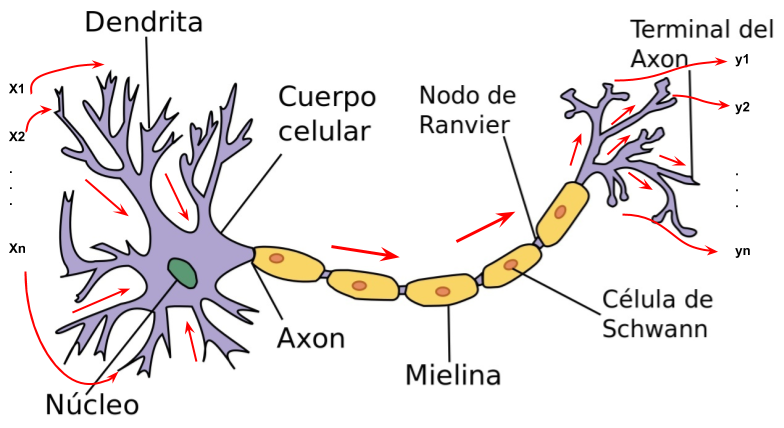
\includegraphics[width=0.95\textwidth, frame]{imagenes/Cap4/neurona}
  \caption{Graphic of a biological neuron. Reproduced from \protect\cite{Reference67}.}
  \label{fig:neurona_real}
  \end{center}
\end{figure}

A brain neuron can receive about 10,000 entries and in turn send its output to hundreds of neurons.
%Una neurona cerebral puede recibir unas 10000 entradas y enviar a su vez su salida a cientas de neuronas.

\vspace{5mm} %5mm vertical space

The connection between neurons is called a \textbf{synapse}, this is not a physical connection, due there is 2 mm. of separation between neurons. These connections are unidirectional, where information's transmission is done electrically inside the neuron and chemically between neurons, thanks to neurotransmitters.
%La conexi\'{o}n entre neuronas se llama \textbf{sinapsis}, esta no es una conexi\'{o}n f\'{i}sica, sino que existe 2 mm. de separaci\'{o}n entre neuronas. Estas conexiones son unidireccionales, donde la transmisi\'{o}n de la informaci\'{o}n se hace de forma el\'{e}ctrica en el interior de la neurona  y de forma qu\'{i}mica entre neuronas, gracias a los neurotransmisores.

\vspace{5mm} %5mm vertical space

An \textbf{artificial neuron} is an elementary processor, because it processes a vector $x(x_{1},x_{2}, ... ,x_{n})$ of inputs and produces a unique response or output. The main elements of an artificial neuron are the following:
%Una \textbf{neurona artificial} es un procesador elemental, debido a que procesa un vector $x(x_{1},x_{2}, ... ,x_{n})$ de entradas y produce una respuesta o salida \'{u}nica. Los elementos principales de una neurona artificial son los siguientes:

\begin{figure}[h!]
  \begin{center}	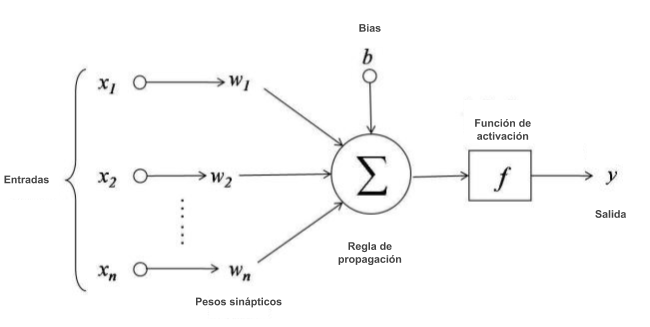
\includegraphics[width=0.95\textwidth, frame]{imagenes/Cap4/neurona_artificial}
  \caption{Graphic of an artificial neuron. Reproduced from \protect\cite{Reference68}.}
  \label{fig:neurona}
  \end{center}
\end{figure}

\begin{itemize}
\item \textbf{Inputs} that receive data from other neurons, these inputs would be dendrites of a biological neuron.
%\item \textbf{Las entradas} que reciben los datos de otras neuronas, estas entradas ser\'{i}an las dendritas de una neurona biol\'{o}gica.
\item \textbf{Synaptic weights} $w_{ij}$. In an artificial neuron, those inputs that come from other neurons are assigned a weight (importance factor). This weight is a numerical value that is modified during the training process of a neural network, and therefore it is here that information that makes the network serve one purpose or another is stored.
%\item \textbf{Los pesos sin\'{a}pticos $w_{ij}$}. En una neurona artificial a aquellas entradas que vienen de otras neuronas se les asigna un peso (factor de importancia). Este peso es un valor num\'{e}rico que se modifica durante el proceso de entrenamiento de una red neuronal, y por lo tanto es aqu\'{i} donde se almacena la informaci\'{o}n que hace que la red sirva para un prop\'{o}sito u otro.
\item \textbf{Propagation Rule}. With inputs and synaptic weights, some type of operation is usually done to obtain the potential postsynaptic value; one of the most common operations is to add up all entries, but taking into account importance (synaptic weight) of each one; This operation is called \textit{weighted sum} \ref{eqn:suma_pon}, however other operations are also possible. Another propagation rule that is usual is Euclidean distance.
%\item \textbf{Regla de propagaci\'{o}n}. Con las entradas y los pesos sin\'{a}pticos, se suele hacer alg\'{u}n tipo de operaci\'{o}n para obtener el valor potencial postsin\'{a}ptico; una de las operaciones m\'{a}s comunes es sumar las entradas, pero teniendo en cuenta la importancia (peso sin\'{a}ptico) de cada una; esta operaci\'{o}n se llama \textit{suma ponderada} \ref{eqn:suma_pon}, sin embargo otras operaciones tambi\'{e}n son posibles. Otra regla de propagaci\'{o}n que es habitual es la distancia euclidiana.
\begin{equation}
h_{i}(t) = \sum_{j}{w_{ij}x_{j}}
\label{eqn:suma_pon}
\end{equation}
\item \textbf{Activation Function}. The value obtained with the propagation rule is filtered through a function known as the \textit{activation function} and is what gives the output of neuron. The activation function is important because it is the one that decides whether a neuron should be activated or not, and if this function is not applied, the output signal of neuron would simply be a linear function.
%\item \textbf{Funci\'{o}n de activaci\'{o}n}. El valor obtenido con la regla de propagaci\'{o}n, se filtra a trav\'{e}s de una funci\'{o}n conocida como \textit{funci\'{o}n de activaci\'{o}n} y es la que da la salida de la neurona. La función de activación es importante debido a que es la que decide si una neurona debe activarse o no, adem\'{a}s si esta función no se aplica la señal de salida de la neurona sería simplemente una función lineal.
\end{itemize}

\subsection{Types of activation functions}

There are different activation functions, then only the most used in field of neural networks will be presented.
%Existen diferentes funciones de activaci\'{o}n, a continuaci\'{o}n solo se presentar\'{a} las m\'{a}s usadas en el \'{a}mbito de las redes neuronales.

\begin{figure}
        \centering
        \fbox{\begin{varwidth}{\textwidth}
        
        \centering
        \begin{subfigure}[h]{0.45\textwidth} 
            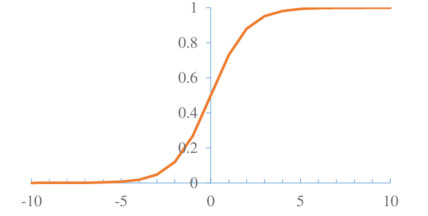
\includegraphics[width=\textwidth]{imagenes/Cap4/sigmoid}
            \caption{Function Sigmoid}
            \label{fig:sigmoid}
        \end{subfigure}       
        \begin{subfigure}[h]{0.45\textwidth} 
            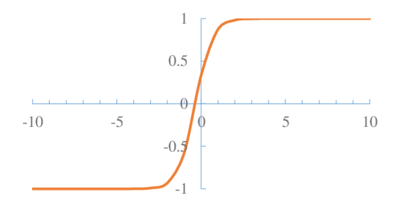
\includegraphics[width=\textwidth]{imagenes/Cap4/tanh}
            \caption{Function Tanh}
            \label{fig:tanh}
        \end{subfigure}
        
        \begin{subfigure}[h]{0.45\textwidth} 
            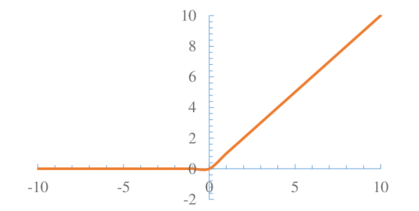
\includegraphics[width=\textwidth]{imagenes/Cap4/relu}
            \caption{Function ReLU}
            \label{fig:relu}
        \end{subfigure}       
        \begin{subfigure}[h]{0.45\textwidth} 
            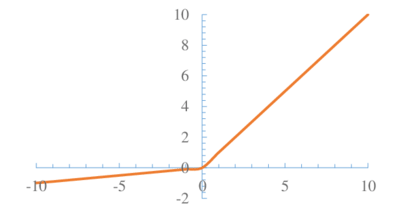
\includegraphics[width=\textwidth]{imagenes/Cap4/l_relu}
            \caption{Function Leaky ReLu}
            \label{fig:l_relu}
        \end{subfigure}
        \begin{subfigure}[h]{0.45\textwidth} 
            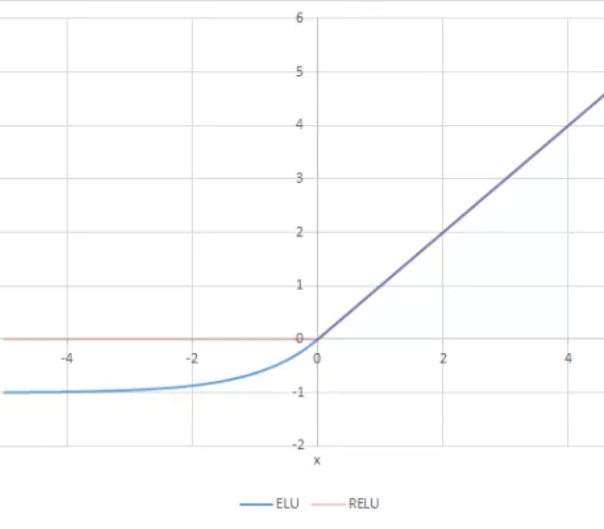
\includegraphics[width=\textwidth]{imagenes/Cap4/elu}
            \caption{Function ELU}
            \label{fig:elu}
        \end{subfigure}
        \end{varwidth}}
        \caption{Activation functions \protect\cite{Reference69}.}
        
		\label{fig:funciones_activacion}
    \end{figure}
    
\subsubsection{Sigmoid activation function (logistics function)}

A sigmoid function is a mathematical function that has a characteristic ''S'' shaped curve or a sigmoid curve that ranges between 0 and 1 (See Figure \ref{fig:sigmoid}), so this function is usually used in models where you need to predict a Probability as an exit. This function is defined by the following formula:
%Una funci\'{o}n sigmoide es una funci\'{o}n matem\'{a}tica que tiene una curva caracter\'{i}stica en forma de ''S'' o una curva sigmoidea que oscila entre 0 y 1 (Ver Figura \ref{fig:sigmoid}), por lo que esta funci\'{o}n suele ser utilizada en modelos donde se necesita predecir una probabilidad como una salida. Esta funci\'{o}n viene definida por siguiente f\'{o}rmula:

\begin{equation}
f(x) = \frac{1}{1+e^{-x}}
\end{equation}

The sigmoid function was successfully applied in problems of binary classification, modeling of logistic regression tasks, as well as other neural network domains, however, it suffers significant drawbacks that include acute wet gradients during backward propagation from deeper hidden layers to input layers, gradient saturation, slow convergence and non-zero centered output, which causes gradient updates to propagate in different directions.
%La funci\'{o}n sigmoide se aplic\'{o} con éxito en problemas de clasificación binaria, modelado de tareas de regresión logística, así como otros dominios de red neuronal, sin embargo, sufre inconvenientes importantes que incluyen gradientes húmedos agudos durante la propagación hacia atrás desde capas ocultas más profundas a las capas de entrada, saturación de gradiente, convergencia lenta y salida no centrada en cero, lo que hace que las actualizaciones de gradiente se propaguen en diferentes direcciones.

\subsubsection{Hyperbolic Tangent Function - Tanh}

It is quite similar to Sigmoid but has a much better performance compared to multilayer neural network training, its nature is nonlinear. This function is centered at 0 and its range is between -1 and 1 (See Figure \ref{fig:tanh}), therefore, its output is defined by:
%Es bastante similar a Sigmoid pero tiene un rendimiento mucho mejor respecto al entrenamiento de redes neuronales multicapa, su naturaleza es no lineal. \'{E}sta funci\'{o}n est\'{a} centrada en 0 y su rango se encuentra entre -1 y 1 (Ver Figura \ref{fig:tanh}), por lo tanto, su salida esta definida por:

\begin{equation}
f(x)=\frac{e^{x}-e^{-x}}{e^{x}+e^{-x}}
\end{equation}
 
Although this function has a better performance than the sigmoid, it could not solve the leakage gradient problem that sigmoid functions have. One of the main advantages of  tangential function is that it produces a zero-centered output, which helps the backward propagation process.   
%Aunque esta funci\'{o}n tenga un mejor rendimiento que la sigmoide, no pudo resolver el problema de gradiente de fuga que tienen las funciones sigmoideas. Una de las principales ventajas de la funci\'{o}n tangencial es que produce una salida centrada a cero, lo cual ayuda al proceso de propagaci\'{o}n hacia atr\'{a}s.

\vspace{5mm} %5mm vertical space

Tangent functions have been used primarily in recurrent neural networks for natural language processing \cite{Reference43} and speech recognition tasks \cite{Reference44}.
%Las funciones de tangente se han utilizado principalmente en redes neuronales recurrentes para el procesamiento del lenguaje natural \cite{Reference43} y tareas de reconocimiento del habla \cite{Reference44}.
    
\subsubsection{Rectified Linear Unit function (ReLU)}

The ReLU function was proposed by Nair and Hinton in 2010, and since then it has been the most widely used activation function for machine learning applications with neural networks. ReLU is a faster learning activation function \cite{Reference46}, so it proved to be the most successful and most used function. This function offers better performance and generalization than sigmoid and tangent functions in learning with neural networks.
%La funci\'{o}n ReLU fue propuesta por Nair y Hinton en 2010, y desde entonces ha sido la funci\'{o}n de activaci\'{o}n m\'{a}s ampliamente utilizada para aplicaciones de aprendizaje autom\'{a}tico con redes neuronales. ReLU es una funci\'{o}n de activaci\'{o}n de aprendizaje m\'{a}s r\'{a}pido \cite{Reference46}, por lo que demostr\'{o} ser la funci\'{o}n m\'{a}s exitosa y m\'{a}s usada. Esta funci\'{o}n ofrece un mejor rendimiento y generalizaci\'{o}n que las funciones sigmoide y tangente en el aprendizaje con redes neuronales.

\vspace{5mm} %5mm vertical space

ReLU represents an almost linear function and, therefore, retains the properties of linear models that makes it easy to optimize, with gradient descent methods.
%ReLU representa una función casi lineal y, por lo tanto, conserva las propiedades de los modelos lineales que lo hace fácil de optimizar, con métodos de descenso de gradiente.

\vspace{5mm} %5mm vertical space

The ReLU activation function performs a threshold operation for each input element where values below zero are set to zero (See Figure \ref{fig:relu}), so ReLU is defined by:
%La función de activación de ReLU realiza una operación de umbral para cada elemento de entrada donde los valores inferiores a cero se establecen en cero (Ver Figura \ref{fig:relu}), por lo que ReLU esta definida por:

\begin{equation}
f(x) = max(0,x) = \left\lbrace
\begin{array}{ll}
\textup{si } x_{i}\geq0 & x_{i}\\
\textup{si } x_{i} < 0 & 0
\end{array}
\right.
\end{equation}

This function rectifies the values of inputs below zero, forcing them to become zero, thereby eliminating leakage gradient problem observed in previous types of activation function. The ReLU function has been used within the hidden units of neural networks.
%Esta función rectifica los valores de las entradas inferiores a cero, obligándolos a convertirse en cero, con lo cual elimina el problema de gradiente de fuga observado en los tipos anteriores de función de activación. La función ReLU se ha usado dentro de las unidades ocultas de las redes neuronales.

\vspace{5mm} %5mm vertical space

The main advantage of using ReLU is that it guarantees a faster calculation, since it does not calculate exponentials and divisions, with an improved general calculation speed \cite{Reference45}. Another property of ReLU is that it introduces the shortage in hidden units, since it reduces values between zero and maximum. However, RELU has the limitation that it is easily overfited compared to sigmoid function, although abandonment technique has been adopted to reduce overfited effect of ReLU and rectified networks improved performance of neural networks.
%La principal ventaja de utilizar ReLU es que garantiza un cálculo más rápido, ya que no calcula exponenciales y divisiones, con una velocidad general de cálculo mejorada \cite{Reference45}. Otra propiedad de ReLU es que introduce la escasez en las unidades ocultas, ya que reduce los valores entre cero y máximo. Sin embargo, ReLU tiene la limitación de que se sobreajusta fácilmente en comparación con la función sigmoidea, aunque se ha adoptado la técnica de abandono para reducir el efecto de sobreajuste de ReLU y las redes rectificadas mejoraron el rendimiento de las redes neuronales.

\vspace{5mm} %5mm vertical space

ReLU has a significant limitation that it is sometimes fragile during training, causing the death of some gradients. This makes some neurons also dead, to solve problems of dead neurons, the Leaky ReLU activation function was proposed.
%ReLU tiene una limitación significativa de que a veces es frágil durante el entrenamiento, causando la muerte de algunos de los gradientes. Esto hace que algunas neuronas también estén muertas, para resolver los problemas de neuronas muertas, se propuso la funci\'{o}n de activaci\'{o}n Leaky ReLU.

\subsubsection{Leaky ReLU (LReLU)}

The year 2013 was proposed as an activation function, this function introduces a small negative slope to ReLU to keep and keep weight updates alive during the propagation process \cite{Reference44}. The parameter $\alpha$ was introduced as a solution to the problems of dead neurons of ReLU. This function calculates gradient with a very small constant value for negative gradient $\alpha$ in the range of 0.01, so LReLU (See Figure \ref{fig:l_relu}) is calculated as:
%Fue propuesta el a\~{n}o 2013 como una funci\'{o}n de activaci\'{o}n, esta funci\'{o}n introduce una peque\~{n}a pendiente negativa a ReLU para mantener y mantener vivas las actualizaciones de peso durante el proceso de propagaci\'{o}n \cite{Reference44}. El par\'{a}metro $\alpha$ fue introducido como una soluci\'{o}n a los problemas de neuronas muertas de ReLU. Esta funci\'{o}n calcula el gradiente con un valor constante muy peque\~{n}o para el gradiente negativo $\alpha$ en el rango de 0.01, por lo que LReLU (Ver Figura \ref{fig:l_relu}) se calcula como:

\begin{equation}
f(x) = \alpha x + x = \left\lbrace
\begin{array}{ll}
\textup{si } x_{i}>0 & x_{i}\\
\textup{si } x_{i} \leq 0 & \alpha x_{i}
\end{array}
\right.
\end{equation}

\subsubsection{Exponential Linear Unit Function (ELU)}

The ELU\footnote{\textbf{ELU, }Exponencial Lineal Unit} function tends to converge the cost to zero faster and produces more accurate results. Unlike other activation functions ELU has an additional alpha constant that should be a positive number.
%La funci\'{o}n ELU\footnote{\textbf{ELU, }Exponencial Lineal Unit} tiende a converger el costo a cero m\'{a}s rapido y produce resultados m\'{a}s precisos. A diferencia de otras funciones de activaci\'{o}n ELU tiene una constante alfa adicional que deber\'{i}a ser un n\'{u}mero positivo.

\vspace{5mm} %5mm vertical space

It is very similar to ReLU since both have an identity function for positive inputs, however in ELU negative inputs it softens slowly until its output is equal $-\alpha$ while in ReLU it softens sharply. ELU function is calculated according to equation \ref{eqn:elu}.
%Es muy similar a ReLU ya que ambas tienen una funci\'{o}n identidad para las entradas positivas, sin embargo en las entradas negativas ELU se suaviza lentamente hasta que su salida es igual $-\alpha$ mientras que en ReLU se suaviza bruscamente. La funci\'{o}n ELU se calcula seg\'{u}n la ecuaci\'{o}n \ref{eqn:elu}.

\begin{equation}
f(x) = \left\lbrace
\begin{array}{ll}
\textup{si } x_{i}>0 & x_{i}\\
\textup{si } x_{i} \leq 0 & \alpha *( e^{x_{i}}-1)
\end{array}
\right.
\label{eqn:elu}
\end{equation}

\subsection{Architecture of the Neural Networks}

A regular neural network consists of a chain of interconnected layers of neurons, these layers are: an input layer, one or several hidden layers and an output layer.
%Una red neuronal regular consiste de una cadena de capas interconectadas de neuronas, estas capas son: una capa de entrada, una o varias capas ocultas y una capa de salida. 

\begin{figure}[h!]
  \begin{center}	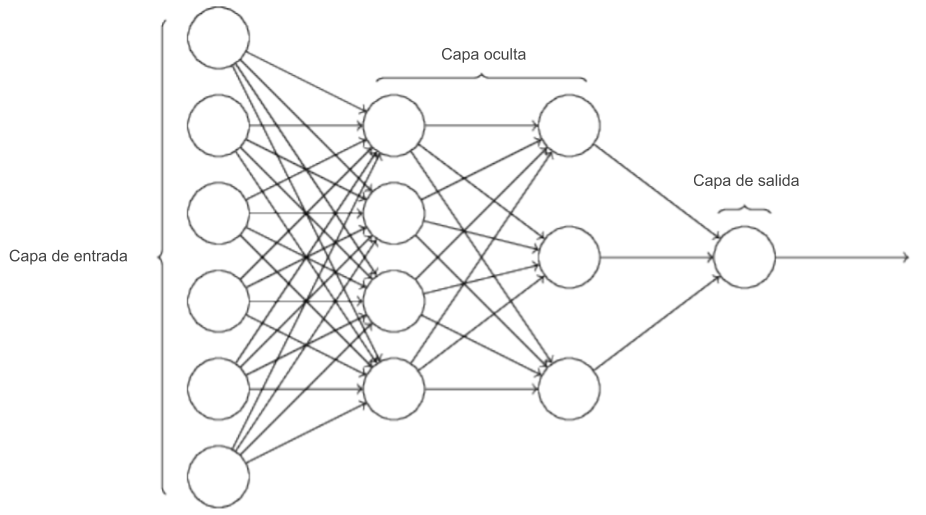
\includegraphics[width=0.95\textwidth, frame]{imagenes/Cap4/arquitectura}
  \caption{Architecture of an artificial neuron. Reproduced from \protect\cite{Reference70}.}
  \label{fig:arquitectura}
  \end{center}
\end{figure}

Figure \ref{fig:arquitectura} is an example of a very simple neural network; In this figure the leftmost layer is called \textbf{input layer}, and the neurons within this layer are called input neurons. The rightmost or \textbf{output layer} contains  output neurons. And finally the two intermediate layers are \textbf{hidden layers} of neural network, these are called that because neurons of this layer are not input or output; A neural network can have one or more hidden layers.
%La figura \ref{fig:arquitectura} es un ejemplo de una red neuronal muy simple; en esta figura la capa m\'{a}s a la izquierda se llama \textbf{capa de entrada}, y las neuronas dentro de esta capa se llaman neuronas de entrada. La capa m\'{a}s a la derecha o de \textbf{salida} contiene las neuronas de salida. Y por \'{u}ltimo las dos capas intermedias son las \textbf{capas ocultas} de la red neuronal, estas se llaman as\'{i} debido a que las neuronas de esta capa no son de entrada o de salida; una red neuronal puede tener una o m\'{a}s capas ocultas.

\vspace{5mm} %5mm vertical space

Unlike the human brain, an Artificial Neural Network has a fairly strict predefined structure, connections between neurons are always forward (feedforward): connections range from the neurons of a given layer to neurons of next layer, that is, There are no side connections or back connections. This means that a neuron that was activated in layer 3 cannot activate a neuron in layer 2 or earlier.
%A diferencia del cerebro humano, una Red Neuronal Artificial tiene una estructura predefinida bastante estricta, las conexiones entre neuronas son siempre hacia adelante (feedforward): las conexiones van desde las neuronas de una determinada capa hacia las neuronas de la siguiente capa, es decir, no existen conexiones laterales ni conexiones hacia atr\'{a}s. Esto significa que una neurona que fue activada en la capa 3 no puede activar a una neurona de la capa 2 o anterior.

\subsection{Learning process of Neural Networks}

A key feature of neural networks is their iterative learning process, that is, each sample of training set is presented to the network, one at a time, so that the weights associated with input values are adjusted each time. During this learning phase, the network trains by adjusting the weights to predict a correct output for input samples.
%Una caracter\'{i}stica clave de las  redes neuronales es su proceso de aprendizaje iterativo, es decir, cada ejemplo del conjunto de entrenamiento se presenta a la red, uno a la vez, con lo que los pesos asociados con los valores de entrada se ajustan cada vez. Durante esta fase de aprendizaje, la red se entrena ajustando los pesos para predecir una salida correcta para las muestras de entrada.

\vspace{5mm} %5mm vertical space

Neural networks have the advantage of having a high tolerance for noisy data, as well as a high capacity to classify patterns with which they have not been trained. The most popular neural network training technique is the backpropagation algorithm.
%Las redes neuronales tienen la ventaja de tener una alta tolerancia a los datos ruidosos, como tambi\'{e}n una alta capacidad para clasificar patrones con los que no han sido entrenados. La t\'{e}cnica de entrenamiento de redes neuronales m\'{a}s popular es el \textbf{algoritmo de retropropagaci\'{o}n} (Backpropagation). 

\vspace{5mm} %5mm vertical space

Once the structure of a network is defined for a particular application, it is ready to be trained. To begin this process, initial weights are chosen at random, and then proceed with training (learning).
%Una vez que se define la estructura de una red para una aplicaci\'{o}n en particular, est\'{a} lista para ser capacitada. Para comenzar este proceso, los pesos iniciales se eligen al azar, para luego proceder con el entrenamiento (aprendizaje). 

\subsubsection{Backpropagation}

A neural network propagates the signal of input data forward through its parameters at the time of decision; and then spread back the information about the error, so that parameters can be altered. This happens by following steps below:
%Una red neuronal propaga la se\~{n}al de los datos de entrada hacia adelante a trav\'{e}s de sus par\'{a}metros en el momento de la decisi\'{o}n; para luego propagar hacia atr\'{a}s la informaci\'{o}n sobre el error, para que se pueda alterar los par\'{a}metros. Esto sucede siguiendo los siguientes pasos:

\begin{itemize}
\item The network guesses output data, using its parameters.
\item The network measures its accuracy with a loss function.
\item The error is propagated backwards to adjust the wrong parameters.
%\item La red adivina los datos de salida, usando sus par\'{a}metros.
%\item La red mide su precisi\'{o}n con una funci\'{o}n de p\'{e}rdida.
%\item El error es propagado hacia atr\'{a}s para ajustar los par\'{a}metros equivocados.
\end{itemize}

Therefore it can be said that Backpropagation algorithm takes the error associated with an erroneous assumption by neural network, and uses that error to adjust parameters of neural network in the direction that generates the least error.
%Por lo tanto se puede decir que el algoritmo de Backpropagation toma el error asociado con una suposición errónea por parte de la red neuronal, y usa ese error para ajustar los parámetros de la red neuronal en la dirección que genere un menor error.

\section{Types of Neural Networks}

\subsection{Autoencoders}

An Autoencoder is an Artificial Neural Network used for unsupervised machine learning, it is trained to reconstruct its own inputs, that is, predict the value of output $\hat{x}$ given an input $x$ via a hidden layer $h$, see Figure \ref{fig:autoencoder1}. Autoencoders are usually used for dimensionality reduction and feature learning.
%Un Autoencoder es una Red Neuronal Artificial usada para aprendizaje autom\'{a}tico no supervisado, esta entrenada para reconstruir sus propias entradas, es decir, predecir el valor de la salida $\hat{x}$ dada una entrada $x$ v\'{i}a una capa oculta $h$, ver Figura \ref{fig:autoencoder1}. Los autoencoders suelen ser usados para reducci\'{o}n de dimensionalidad y aprendizaje de caracter\'{i}sticas. 

\begin{figure}[h!]
  \begin{center}	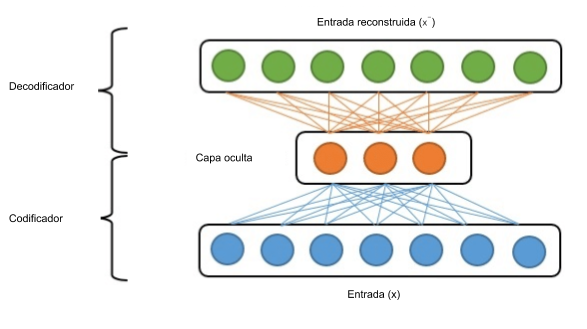
\includegraphics[width=0.95\textwidth, frame]{imagenes/Cap4/autoencoder}
  \caption{Graphic of an Autoencoder (Own elaboration).}
  \label{fig:autoencoder1}
  \end{center}
\end{figure}

Autoencoders are composed of two parts: the encoder and decoder. Encoder learns a compressed representation of input data, this can be defined with the coding function $h=encoder(x)$, which is defined by a linear or nonlinear function. If function of encoder is non-linear, auto-encoder will be able to learn more features than a linear PCA. The purpose of decoder is to reconstruct its own input via the decoding function, $\hat{x} = decoder(h)$.
%Los autoencoders est\'{a}n compuestos de dos partes: el codificador y decodificador. El codificador aprende una representaci\'{o}n compresa de los datos de entrada, este puede ser definido con la funci\'{o}n de codificaci\'{o}n $h=encoder(x)$, el cual es definido por una funci\'{o}n lineal o no lineal. Si la funci\'{o}n del codificador es no lineal el autoencoder ser\'{a} capaz de aprender m\'{a}s caracter\'{i}sticas que un PCA lineal. El prop\'{o}sito del decodificador es reconstruir su propia entrada v\'{i}a la funci\'{o}n de decodificaci\'{o}n, $\hat{x} = decodificador(h)$.

\vspace{5mm} %5mm vertical space

The difference between input and reconstructed input is the reconstruction error. During training, autoencoder minimizes the reconstruction error as an objective function. Autoencoders are often used for data generation as generative models. Decoder of an autoencoder can generate an output given an artificially assigned compressed representation.
%La diferencia entre la entrada y la entrada reconstruida es el \textbf{error de reconstrucción}. Durante el entrenamiento, el autoencoder minimiza el error de reconstrucción como una función objetivo. Los autoencoders se usan a menudo para la generación de datos como modelos generativos. El decodificador de un autoencoder puede generar una salida dada una representación comprimida asignada artificialmente.

\subsection{Convolutional neural networks}

For some types of data, specifically for images, conventional neural networks are not well adapted; which implies that in the study \citeA{Reference48} propose convolutional neural networks (CNN\footnote{\textbf{CNN,} Convolutional Neural Network}) to solve this problem. CNNs have revolutionized image processing and eliminated manual feature extraction. A CNN acts directly on matrices, or even on tensors for images with three RGB color channels; so currently, CNNs are widely used for image classification, object recognition, face recognition, among others.
%Para algunos tipos de datos, especificamente para im\'{a}genes, las redes neuronales convencionales no est\'{a}n bien adaptadas; lo cual conlleva que en el estudio \citeA{Reference48} propongan las redes neuronales convolucionales (CNN\footnote{\textbf{CNN,} Convolutional Neural Network}) para solucionar ese problema. Las CNN han revolucionado el procesamiento de im\'{a}genes y han eliminado la extracci\'{o}n manual de caracter\'{i}sticas. Una CNN act\'{u}a directamente en matrices, o incluso en tensores para im\'{a}genes con tres canales de color RGB; por lo que actualmente, las CNN se usan ampliamente para la clasificaci\'{o}n de im\'{a}genes, reconocimiento de objetos, reconocimiento de rostros, entre otros.

\vspace{5mm} %5mm vertical space

CNNs not only provide better performance compared to other detection algorithms; but even in some cases they outnumber humans, such as in classification of objects in specific categories such as particular breed of a dog or a species of bird \cite{Reference49}.
%Las CNN no solo brindan un mejor rendimiento en comparaci\'{o}n con otros algoritmos de detecci\'{o}n; sino que incluso en algunos casos superan a los humanos, como por ejemplo en la clasificaci\'{o}n de objetos en categor\'{i}as espec\'{i}ficas como la raza particular de un perro o una especie de ave \cite{Reference49}.

\vspace{5mm} %5mm vertical space

By stacking multiple and different layers in a CNN, complex architectures are created for classification problems. The four types of layers that are most common are: convolution layer, grouping/subsampling layer, nonlinear layer and fully connected layer. An example of a CNN can be seen in Figure \ref{fig:cnn}, where the first and third layers are convolutional layers, the second and fourth are subsampling layers and finally the fifth and sixth layers with completely connected layers.
%Al apilar múltiples y diferentes capas en una CNN, se crean arquitecturas complejas para los problemas de clasificación. Los cuatro tipos de capas que son más comunes son: capa de convolución, capa de agrupación/submuestreo, capa no lineal y capa completamente conectada. En la Figura \ref{fig:cnn} se puede ver un ejemplo de una CNN, donde la primera y tercera capa son capas convolucionales, la segunda y la cuarta son capas de submuestreo y por \'{u}ltimo la quinta y la sexta capa con capas completamente conectadas. 

\begin{figure}[h!]
  \begin{center}	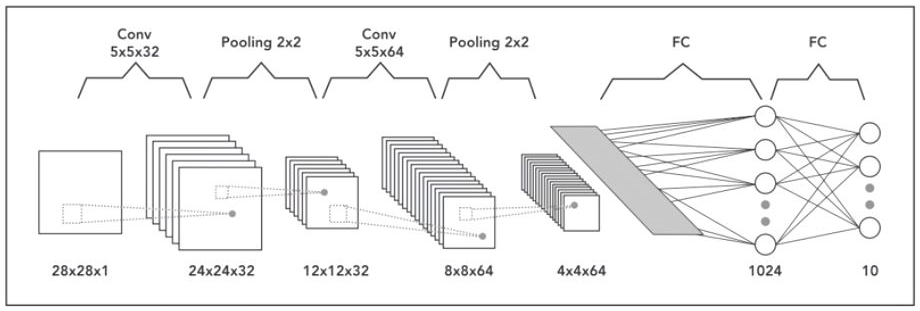
\includegraphics[width=0.95\textwidth]{imagenes/Cap4/cnn}
  \caption{Architecture of a Convolutional Neural Network (CNN) \protect\cite{Reference71}.}
  \label{fig:cnn}
  \end{center}
\end{figure}

\subsection{Recurrent neural networks}

To understand the importance of time series, the following analogy can be taken, human beings do not start to think from scratch every second, so when reading a document each word is understood based on understanding of the previous words, that is to say , everything is not eliminated and you start thinking of zero every time, given this statement you can say that thoughts of human beings have persistence.
%Para entender la importancia de las series de tiempo se puede tomar la siguiente analog\'{i}a, los seres humanos no comienzan a pensar desde cero cada segundo, por lo que al leer un documento se comprende cada palabra bas\'{a}ndose en la comprensi\'{o}n de las palabras anteriores, es decir, no se elimina todo y se empieza a pensar de cero cada vez, dada \'{e}sta afirmaci\'{o}n se puede decir que los pensamientos de los seres humanos tienen persistencia.

\vspace{5mm} %5mm vertical space

Traditional neural networks do not have data persistence, which for some specific problems, including the one of this work, is a major deficiency. In order to solve these types of problems, Recurrent Neural Networks (RNN\footnote{\textbf{RNN,} Recurrent Neural Network}) appear, which are a type of artificial neural network proposed in the 80s (\citeNP{Reference34}; \citeNP{Reference35}; \citeNP{Reference36}) designed to recognize patterns in data streams, such as text, genomes, handwriting, numerical time series data emanating from sensors, among others
%Las redes neuronales tradicionales no tienen persistencia de los datos, lo que para algunos problemas en concreto, incluyendo el que se aborda en este trabajo, es una gran deficiencia. Con el fin de resolver este tipo de problemas aparecen las Redes Neuronales Recurrentes (RNN\footnote{\textbf{RNN,} Recurrent Neural Network}), las cuales son un tipo de red neuronal artificial propuesta en los a\~{n}os 80 (\citeNP{Reference34}; \citeNP{Reference35}; \citeNP{Reference36}) dise\~{n}ada para reconocer patrones en secuencias de datos, como texto, genomas, escritura a mano, datos de series de tiempo num\'{e}ricos que emanan de sensores, entre otros.

\vspace{5mm} %5mm vertical space

RNNs are a particular family of neural networks where the network contains one or more feedback connections, so that the activation of a group of neurons can flow in a loop. This property allows model to retain information about past, which allows it to discover temporal correlations between events that are far from each other in data.
%Las RNN son una familia particular de redes neuronales donde la red contiene una o más conexiones de retroalimentación, de modo que la activación de un grupo de neuronas puede fluir en un bucle. Esta propiedad hace que el modelo pueda retener informaci\'{o}n sobre el pasado, lo que le permite descubrir correlaciones temporales entre eventos que est\'{a}n muy lejos unos de otros en los datos.

\vspace{5mm} %5mm vertical space

RNN have a certain memory of what happened previously in a sequence of data, this helps system to gain context of data. Theoretically it is said that RNN has infinite memory, that is, these types of networks have ability to look back indefinitely; However, in practice you can only look back a few last steps.
%Las RNN tienen una cierta memoria de lo que sucedi\'{o} anteriormente en una secuencia de datos, esto ayuda al sistema a ganar contexto de los datos. Te\'{o}ricamente se dice que las RNN tiene memoria infinita, es decir, este tipo de redes tienen la capacidad de mirar hacia atr\'{a}s indefinidamente; sin embargo en la pr\'{a}ctica s\'{o}lo se puede mirar atr\'{a}s unos \'{u}ltimos pasos.

\begin{figure}[h!]
  \begin{center}	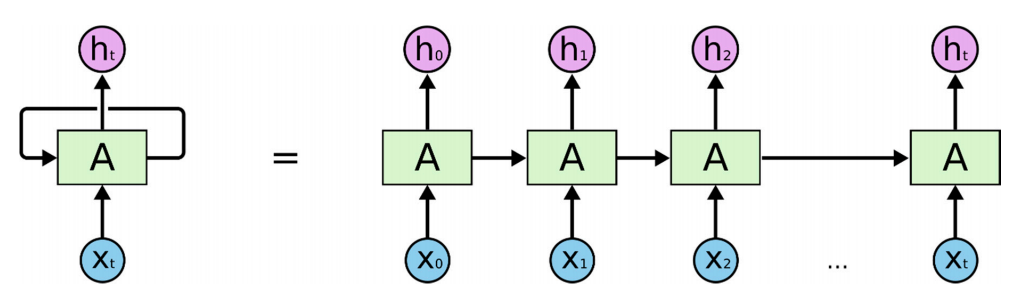
\includegraphics[width=0.95\textwidth, frame]{imagenes/Cap4/rnn}
  \caption{Sequential processing in a recurrent neural network (RNN) \protect\cite{Reference53}.}
  \label{fig:rnn}
  \end{center}
\end{figure}

Figure \ref{fig:rnn} illustrates a simple RNN with an input unit, an output unit and a recurring hidden unit expanded in a complete network, where xt is input in the time step t and t is output in the time step t. On the other hand, in training process, RNNs use the Backpropagation algorithm over time (BPTT\footnote{\textbf{BPTT,} Backpropagation Through The Time}). The BPTT process uses a backward, layer by layer, work approach of final output of network, adjusting the weights of each unit according to calculated unit portion of total output error. The repetition of information loops results in large updates of neural network model weights and leads to an unstable network due to accumulation of error gradients during the update process. Therefore, BPTT is not efficient enough to learn a pattern of long-term dependence due to disappearance of gradient and the explosion of gradient problems \cite{Reference50}. To overcome disappearance and explosion gradient problems that standard RNNs have, LSTM and GRU can be used \cite{Reference51}.
%En la Figura \ref{fig:rnn} se ilustra una simple RNN con una unidad de entrada, una unidad de salida y una unidad oculta recurrente expandida en una red completa, donde $x_{t}$ es la entrada en el paso de tiempo $t$ y $y_{t}$ es la salida en el paso de tiempo $t$. Por otra parte en el proceso de entrenamiento las RNN usan el algoritmo de Backpropagation a trav\'{e}s del tiempo (BPTT\footnote{\textbf{BPTT,} Backpropagation Through The Time}). El proceso BPTT utiliza un enfoque de trabajo hacia atrás, capa por capa, de la salida final de la red, ajustando los pesos de cada unidad de acuerdo con la porción calculada de la unidad del error de la salida total. La repetición de los bucles de información da como resultado grandes actualizaciones de los pesos del modelo de red neuronal y conduce a una red inestable debido a la acumulación de gradientes de error durante el proceso de actualización. Por lo tanto, BPTT no es lo suficientemente eficiente como para aprender un patrón de dependencia a largo plazo debido a la desaparición del gradiente y la explosión de los problemas del gradiente \cite{Reference50}. Para superar los problemas de gradiente de desaparición y explosión que tienen las RNN estándar, se pueden usar LSTM y GRU \cite{Reference51}.

\subsection{LSTM}

LSTM\footnote{\textbf{LSTM,} Long Short-Term Memory} is an evolution of RNN, it was introduced by Hochreiter and Schmidhuber in \citeyear{Reference52} to board the problems of standard RNNs that were mentioned before, adding additional interactions per module (or cell). LSTMs are a special type of RNN, capable of learning long-term dependencies and remembering information for extended periods by default.
%LSTM\footnote{\textbf{LSTM,} Long Short-Term Memory} es una evoluci\'{o}n de RNN, fue introducida por Hochreiter y Schmidhuber en \citeyear{Reference52} para abordar los problemas de las RNN est\'{a}ndar que fueron mencionados antes, agregando interacciones adicionales por m\'{o}dulo (o celda). Los LSTM son un tipo especial de RNN, capaces de aprender dependencias a largo plazo y recordar información por períodos prolongados por defecto.

\vspace{5mm} %5mm vertical space

The LSTM model is organized in form of a chain structure. However, the repetition module has a different structure. Instead of a single neural network like a standard RNN, it has four interactive layers with a unique method of communication. The LSTM's structure is shown in Figure 3.8.
%El modelo LSTM está organizado en forma de estructura de cadena. Sin embargo, el módulo de repetición tiene una estructura diferente. En lugar de una sola red neuronal como un RNN estándar, tiene cuatro capas interactivas con un método único de comunicación. La estructura de la red neuronal LSTM se muestra en la Figura \ref{fig:lstm}.

\begin{figure}[h!]
  \begin{center}	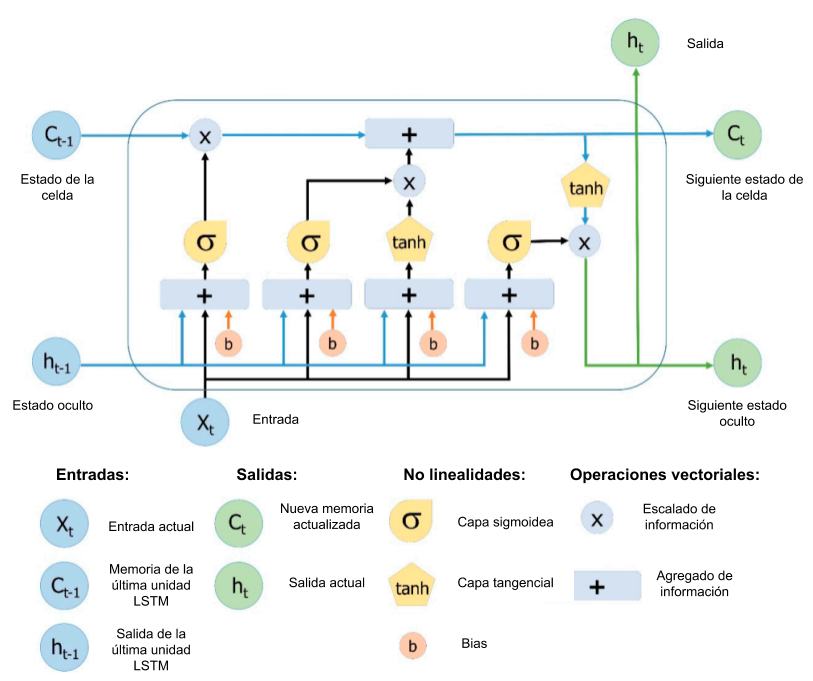
\includegraphics[width=0.95\textwidth, frame]{imagenes/Cap4/lstm}
  \caption{LSTM structure. Played from Yan \protect\cite{Reference54}.} 
  \label{fig:lstm}
  \end{center}
\end{figure}

A typical LSTM network is made up of memory blocks called cells. Two states are transferred to next cell, the state of cell and hidden state. The \textbf{cell's state} is the main chain of data flow, which allows data to flow forward, essentially, without changes. However, some linear transformations may occur. Data can add or remove the cell's state through sigmoid gates.
%Una t\'{i}pica red LSTM esta compuesta por bloques de memoria llamados celdas. Dos estados se transfieren a la siguiente celda, el estado de la celda y el estado oculto. El \textbf{estado de la celda} es la cadena principal del flujo de datos, lo que permite que los datos fluyan hacia adelante, esencialmente, sin cambios. Sin embargo, pueden ocurrir algunas transformaciones lineales. Los datos pueden agregar o eliminar el estado de la celda a trav\'{e}s de puertas sigmoideas.

\vspace{5mm} %5mm vertical space

A door is similar to a layer or a series of matrix operations, which contains different individual weights. LSTMs are designed to avoid the problem of long-term dependence because it uses doors to control memorization process.
%Una puerta es similar a una capa o una serie de operaciones matriciales, la cual contiene diferentes pesos individuales. Los LSTM est\'{a}n dise\~{n}ados para evitar el problema de dependencia a largo plazo porque utiliza puertas para controlar el proceso de memorizaci\'{o}n. 

\subsection{GRU}

GRU\footnote{\textbf{GRU, }Gated Recurrent Unit} was first designed by Kyunghyun Cho in (2014a). This RNN structure only contains two doors. The update door controls information that flows into memory, while the reset door controls information that flows out of memory. Similar to LSTM, GRU has gate units that modulate flow of information within the unit; however, without having a separate memory cell. One could say that GRU is a slightly more simplified variant of RNN that often offers comparable performance to LSTM and is significantly faster to calculate.
%GRU\footnote{\textbf{GRU, }Gated Recurrent Unit} fue dise\~{n}ado por primera vez por Kyunghyun Cho en \citeyear{Reference55}. Esta estructura de RNN s\'{o}lo contiene dos puertas. La puerta de actualizaci\'{o}n controla la informaci\'{o}n que fluye hacia la memoria, mientras que la puerta de reinicio controla la informaci\'{o}n que fluye fuera de la memoria. De manera similar a la LSTM, GRU tiene unidades de compuerta que modulan el flujo de informaci\'{o}n dentro de la unidad; sin embargo, sin tener una celda de memoria separada. Se podr\'{i}a decir que GRU es una variante de RNN un poco m\'{a}s simplificada que a menudo ofrece un rendimiento comparable a LSTM y es significativamente m\'{a}s r\'{a}pido de calcular.

\vspace{5mm} %5mm vertical space

In summary, GRUs have following two distinctive characteristics:
%En resumen, las GRU tienen las siguientes dos caracter\'{i}sticas distintivas:

\begin{itemize}
\item Reset doors help capture short-term dependencies in time series.
\item Update doors help capture long-term dependencies in time series.
%\item Las \textbf{puertas de reinicio} ayudan a capturar dependencias a corto plazo en series de tiempo.
%\item Las \textbf{puertas de actualizaci\'{o}n} ayudan a capturar dependencias a largo plazo en series de tiempo.
\end{itemize}

\begin{figure}[h!]
  \begin{center}	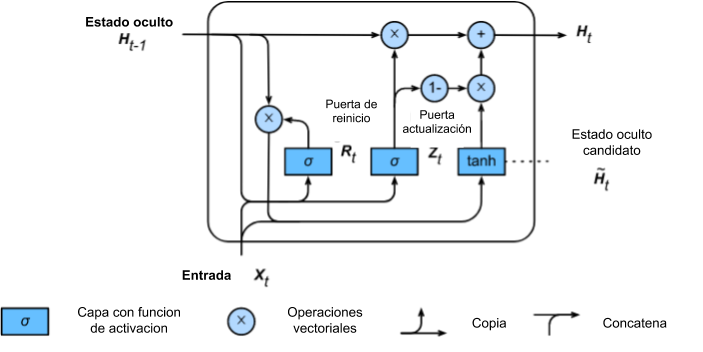
\includegraphics[width=0.95\textwidth, frame]{imagenes/Cap4/gru}
  \caption{GRU structure. Reproduced from \protect\cite{Reference56}.} 
  \label{fig:gru}
  \end{center}
\end{figure}


\section{Anomaly detection techniques}

There are several approaches available for anomaly detection, in this section some of the most used algorithms will be described.
%Existen varios enfoques disponibles para la detección de anomalías, en esta secci\'{o}n se describir\'{a} algunos de los algoritmos m\'{a}s usados.

\subsection{One-Class SVM}

One-Class SVM\footnote{\textbf{SVM, }Support Vector Machine} (OC-SVM) is a widely used approach to discover anomalies in an unsupervised manner (Schölkopf and Smola, 2002). OC-SVMs are one of the most widely used semi-supervised learning techniques, because it gives good results even for large data sets. However, this algorithm has the disadvantage that it requires a lot of time and memory in practice and its complexity grows quadratically with number of records.
%One-Class SVM\footnote{\textbf{SVM, }Support Vector Machine} (OC-SVM) es un enfoque ampliamente utilizado para descubrir anomal\'{i}as de forma no supervisada \cite{Reference59}. Las OC-SVM son una de las técnicas de aprendizaje semi-supervisado más utilizadas, debido a que da buenos resultados incluso para conjuntos de datos de alta dimensión. Sin embargo, este algoritmo tiene la desventaja de que requiere mucho tiempo y memoria en la práctica y su complejidad crece de forma cuadrática con el número de registros.

\vspace{5mm} %5mm vertical space

This algorithm is only trained with positive examples (normal classes). The general idea of this algorithm is to transform the attribute space and draw a divisional hyperplane so that observations are as far as possible from origin, as can be seen in Figure \ref{fig:oc-svm}.
%Este algoritmo s\'{o}lo se entrena con ejemplos positivos (clases normales). La idea general de \'{e}ste algoritmo es transformar el espacio de atributos y dibujar un hiperplano divisorio para que las observaciones se encuentren lo m\'{a}s lejos posible del origen, como se puede observar en la Figura \ref{fig:oc-svm}.

\begin{figure}[h!]
  \begin{center}	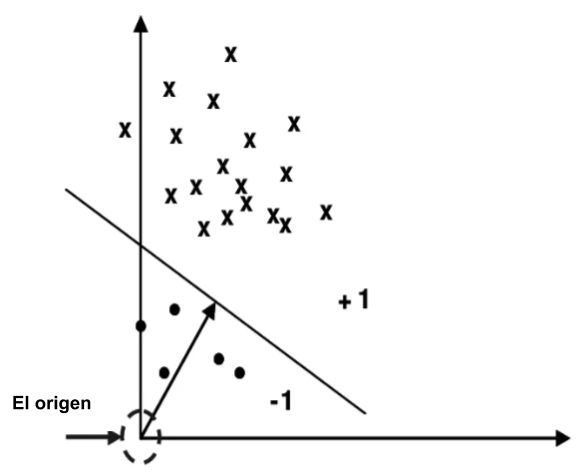
\includegraphics[width=0.45\textwidth, frame]{imagenes/Cap4/oc-svm}
  \caption{One-Class SVM. Reproduced from \protect\cite{Reference72}} 
  \label{fig:oc-svm}
  \end{center}
\end{figure}

\vspace{5mm} %5mm vertical space

As a result, a margin is obtained, on one side of which observations of  training sample are grouped as densely as possible (normal observations $\hat{y_{i}} = 1$), and on the other, abnormal values are found ( $\hat{y_{i}} = -1$ ) , not similar to what the algorithm saw during training.
%Como resultado, se obtiene un margen, en un lado del cual las observaciones de la muestra de entrenamiento se agrupan lo más densamente posible (observaciones normales $\hat{y_{i}} = 1$) , y en el otro, se encuentran los valores anormales ( $\hat{y_{i}} = -1$ ), no similares a lo que el algoritmo vi\'{o} durante el entrenamiento.

\subsection{Isolation Forest}

This model is used in a scenario similar to One Class SVM, specifically in an unsupervised environment. The isolation forest takes a different approach to the OC SVM, since instead of grouping normal data, it tries to isolate the anomalous data.
%Este modelo se usa en un escenario similar al SVM de una clase, específicamente en un entorno no supervisado. El bosque de aislamiento adopta un enfoque diferente del SVM de una clase, ya que en lugar de agrupar datos normales, trata de aislar los datos anómalos.

\vspace{5mm} %5mm vertical space

The basic component of Isolation Forest is the isolation tree, which is a simple binary tree where in each $T_{i}$ node both characteristic and threshold for division rule are randomly selected. An existing node stops generating children if and only if there is only one example following the division rule for that specific route (which means that the example has been isolated) or a maximum height has been reached. This means that at the end of the training process we will have a completely over-adjusted random classification tree, which can be used for anomaly detection purposes. The main intuition of this algorithm is that if an example is anomalous, it will be isolated after some cuts in features space, which translates into having a low height in isolation tree.
%El componente básico del Isolation Forest (Bosque de aislamiento) es el árbol de aislamiento, que es un árbol binario simple donde en cada nodo $T_{i}$ tanto la característica como el umbral para la regla de división se seleccionan aleatoriamente. Un nodo existente deja de generar hijos si y solo si solo hay un ejemplo siguiendo la regla de división para esa ruta específica (lo que significa que el ejemplo se ha aislado) o se ha alcanzado una altura máxima. Esto significa que al final del proceso de capacitación tendremos un árbol de clasificación aleatorio completamente sobreajustado, que puede usarse para fines de detección de anomalías. La intuición principal de este algoritmo es que si un ejemplo es anómalo, se aislará después de algunos cortes en el espacio de características, lo que se traduce en tener una baja altura en el árbol de aislamiento.

\vspace{5mm} %5mm vertical space

Unlike other methods such as grouping or classification, isolation forests do not learn a profile of what is normal, but instead directly attack anomalies. No distance metric is used in this algorithm which saves time in calculations; So isolation forests have a linear temporal complexity.
%A diferencia de otros métodos como la agrupación o clasificación, los bosques de aislamiento no aprenden un perfil de lo que es normal, sino que atacan directamente las anomalías. No se utiliza métrica de distancia en este algoritmo lo cual ahorra tiempo en los cálculos; por lo que los bosques de aislamiento tienen una complejidad temporal lineal. 

\vspace{5mm} %5mm vertical space	

A comparison of the ability of Isolation Forest and One-Class SVM algorithms to cope with different two-dimensional data sets is presented in Figure \ref{fig:comparacion}, with the aim of giving some intuition about behavior of these algorithms.
%En la Figura \ref{fig:comparacion} se presenta una comparaci\'{o}n de la capacidad de los algoritmos Isolation Forest y One-Class SVM para hacer frente a diferentes conjuntos de datos de dos dimensiones, con el objetivo de dar cierta intuici\'{o}n acerca del comportamiento de estos algoritmos.

\begin{figure}[h!]
  \begin{center}	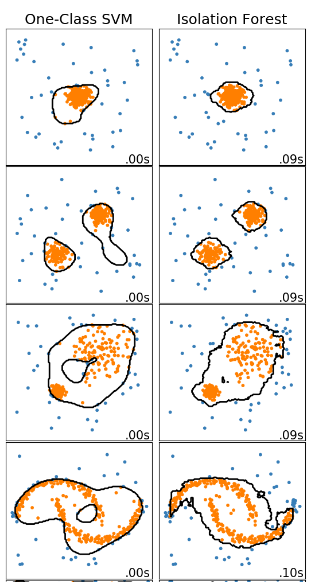
\includegraphics[width=0.43\textwidth, frame]{imagenes/Cap4/comp_if_ocsvm}
  \caption{Performance comparison between the One-Clas SVM and Isolation Forest algorithms. Reproduced from \protect\cite{Reference73}.} 
  \label{fig:comparacion}
  \end{center}
\end{figure}

\subsection{Autoencoders}

Today, autoencoders have been widely used in image classification, machine translation and voice processing; This is due to its ability to compress data without supervision. As far as is known, \shortciteA{Reference57} and \shortciteA{Reference58} were the first to propose autocoders for anomaly detection. Since then, the ability of auto-encoders to detect outliers was demonstrated in different domains such as the detection of anomalies in X-rays.
%Hoy en día, los autoencoders se han utilizado ampliamente en la clasificación de imágenes, traducción automática y procesamiento de voz; esto debido a su capacidad de compresión de datos sin supervisión. Hasta donde se sabe, \shortciteA{Reference57} y \shortciteA{Reference58} fueron los primeros que propusieron autocodificadores para la detección de anomalías. Desde entonces, la capacidad de los autoencoders para detectar valores at\'{i}picos se demostró en diferentes dominios como por ejemplo la detecci\'{o}n de anomal\'{i}as en rayos X.

\vspace{5mm} %5mm vertical space

The traditional method of autoencoder-based anomaly detection is mainly based on reconstruction error, considering as anomalies those samples that present a high reconstruction error. In training phase, only normal data is used to train the auto-encoder, in order to minimize the reconstruction error, so that auto-encoder can recognize  characteristics of normal data. In test phase, the trained auto-encoder will be able to reconstruct normal data with small reconstruction errors, but they will fail with anomalous data that auto-encoder has not encountered before and, therefore, have relatively higher reconstruction errors compared to normal data. Therefore, when comparing whether the reconstruction score of an anomaly is above a predefined threshold, auto-encoder will determine if the data presented for test is anomalous \cite{Reference47} (See Figure \ref{fig:autoencoder-anomaly}) . Equation \ref{eqn:threshold} shows how this technique determines what an anomaly is and what is not; where $S_{z}$ represents the reconstruction.
%El m\'{e}todo tradicional de detecci\'{o}n de anomal\'{i}as basada en autoencoder se basa principalmente en el error de reconstrucci\'{o}n, considerando como anomal\'{i}as aquellas muestras que presentan un alto error de reconstrucci\'{o}n. En la fase de entrenamiento, solo se usan datos normales para entrenar el autoencoder, con el objetivo de minimizar el error de reconstrucci\'{o}n, de modo que el autoencoder pueda reconocer las caracter\'{i}sticas de los datos normales. En la fase de prueba, el autoencoder entrenado podr\'{a} reconstruir datos normales con peque\~{n}os errores de reconstrucci\'{o}n, pero fallar\'{a}n con datos an\'{o}malos que el autoencoder no ha encontrado antes y, por lo tanto, tienen errores de reconstrucci\'{o}n relativamente m\'{a}s altos en comparaci\'{o}n a los datos normales. Por lo tanto, al comparar si el puntaje de reconstrucci\'{o}n de una anomal\'{i}a est\'{a} por encima de un umbral (threshold) predefinido, el autoencoder determinar\'{a} si los datos presentados para la prueba son an\'{o}malos \cite{Reference47} (Ver Figura \ref{fig:autoencoder-anomaly}). La ecuaci\'{o}n \ref{eqn:threshold} se observa como esta t\'{e}cnica determina lo que es una anomal\'{i}a y lo que no lo es; donde $S_{z}$ representa el error de reconstrucci\'{o}n.

\begin{equation}
C(z) = \left\lbrace
\begin{array}{ll}
\textup{if } S_{z}\leq \textup{Threshold} & \textup{Normal behavior}\\
\textup{if } S_{z}> \textup{Threshold} & \textup{Anomaly}
\end{array}
\right.
\label{eqn:threshold}
\end{equation}

\begin{figure}[h!]
  \begin{center}	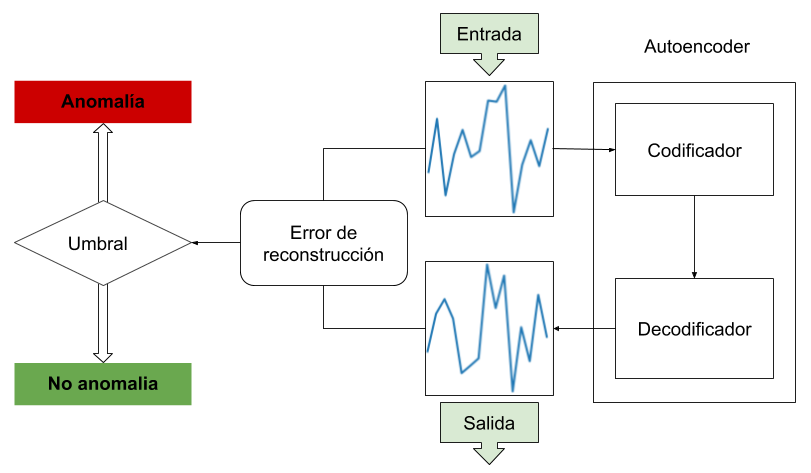
\includegraphics[width=0.95\textwidth, frame]{imagenes/Cap4/autoencoder-anomaly}
  \caption{Detection of anomalies with autoencoder (Own elaboration).} 
  \label{fig:autoencoder-anomaly}
  \end{center}
\end{figure}


\section{Evaluation Metrics}
%https://towardsdatascience.com/metrics-to-evaluate-your-machine-learning-algorithm-f10ba6e38234

Evaluating machine learning algorithms is an essential part of any project, because a model can provide satisfactory results when evaluated with a metric; but it can give a poor result when another metric is used. Classification accuracy is commonly used to measure the performance of a model, however, it is not enough to judge a model. Different types of evaluation metrics will be covered below.
%Evaluar los algoritmos de aprendizaje autom\'{a}tico es una parte esencial para cualquier proyecto, debido a que un modelo puede brindar resultados satisfactorios cuando es evaluado con una m\'{e}trica; pero puede dar un resultado deficiente cuando se utiliza otra m\'{e}trica. Com\'{u}nmente se usa la precisi\'{o}n de clasificaci\'{o}n para medir el rendimiento de un modelo, sin embargo, no es suficiente para juzgar un modelo. A continuaci\'{o}n se cubrir\'{a} diferentes tipos de m\'{e}tricas de evaluaci\'{o}n.

\subsection{Precisi\'{o}n de clasificaci\'{o}n (accuracy)}

La precisi\'{o}n de clasificaci\'{o}n, conocida tambi\'{e}n con el nombre de precisi\'{o}n, es la relaci\'{o}n entre el n\'{u}mero de predicciones correctas y el n\'{u}mero total de muestras de entrada.

\begin{equation}
\textup{Precisi\'{o}n} = \frac{\textup{N\'{u}mero de predicciones correctas}}{\textup{N\'{u}mero total de predicciones realizadas}}
\end{equation}

Esta m\'{e}trica funciona bien si hay el mismo n\'{u}mero de muestras que pertenecen a cada clase; por ejemplo, si se considera que se tiene un conjunto de datos que contiene 98\% de muestras que pertenecen a la clase A y 2\% que pertenecen a la clase B, el modelo podr\'{i}a obtener f\'{a}cilmente un 98\% de precisi\'{o}n de entrenamiento simplemente prediciendo cada muestra de entrenamiento como clase A. 

\vspace{5mm} %5mm vertical space

Esto conlleva que la precisi\'{o}n puede dar la falsa sensaci\'{o}n de lograr una alta precisi\'{o}n, lo cual se convierte en un verdadero problema si se trata problemas que conllevan la detecci\'{o}n de cosas de alto riesgo; por ejemplo, de una enfermedad rara pero mortal ya que el costo de no diagnosticar la enfermedad de una persona enferma es mucho mayor que el costo de enviar a una persona sana a realizarce  m\'{a}s an\'{a}lisis.

\subsection{P\'{e}rdida logar\'{i}tmica (Logarithmic Loss)}

La p\'{e}rdida logar\'{i}tmica, conocida tambi\'{e}n como \textit{Log Loss}, funciona penalizando las clasificaciones falsas, adem\'{a}s tiene un buen rendimiento para la clasificaci\'{o}n de varias clases. Cuando se trabaja con Log Loss, el clasificador debe asignar una probabilidad a cada clase de todas las muestras; suponiendo que hay $N$ muestras que pertenecen a clases $M$, Log Loss se calcula seg\'{u}n la siguiente ecuaci\'{o}n:

\begin{equation}
LogarithmicLoss = \frac{-1}{N}\sum_{i=1}^{N}\sum_{j=1}^{M} y_{ij}*log(p_{ij})
\end{equation}

donde:
\\
$y_{ij}$, indica si la muestra $i$ pertenece a la clase $j$ o no.\\
$p_{ij}$, indica la probabilidad de que la muestra $i$ pertenezca a la clase $j$.

\vspace{5mm} %5mm vertical space

Log Loss no tiene l\'{i}mite superior y existe en el rango $[0, \infty )$. Cuando se obtiene un Log Loss cercano a 0 indica una mayor precisi\'{o}n, mientras que si est\'{a} lejos de 0 indica una menor precisi\'{o}n. En general se puede decir que minimizar Log Loss proporciona una mayor precisi\'{o}n para el clasificador.

\subsection{Matriz de confusi\'{o}n}

La matriz de confusi\'{o}n, tambi\'{e}n llamada matriz de error, es el m\'{e}todo m\'{a}s com\'{u}n para evaluar la exactitud de un resultado de clasificaci\'{o}n \cite{Reference61}. Esta matriz es una tabulaci\'{o}n cruzada de los datos esperados y los resultados de la clasificaci\'{o}n del modelo. El n\'{u}mero de columnas y filas es igual al n\'{u}mero de categor\'{i}as de la clasificaci\'{o}n y de ellas se derivan diferentes medidas estad\'{i}sticas.

\begin{table}[H]

\centering
\begin{center}
\begin{tabular}{ll|c|c|}
\cline{3-4}
                                                        &                                              & \multicolumn{2}{c|}{\textbf{Predicci\'{o}n}}                                                          \\ \cline{3-4} 
                                                        &                                              & \textbf{Clase Positiva}                         & \textbf{Clase Negativa}                         \\ \hline
\multicolumn{1}{|c|}{}                                  & \multicolumn{1}{c|}{\textbf{Clase Positiva}} & \cellcolor[HTML]{AADD99}Verdadero Positivo (VP) & \cellcolor[HTML]{FFCE93}Falso Negativo (FN)     \\ \cline{2-4} 
\multicolumn{1}{|c|}{\multirow{-2}{*}{\textbf{Reales}}} & \multicolumn{1}{c|}{\textbf{Clase Negativa}} & \cellcolor[HTML]{DF9F9F}Falso Positivo (FP)     & \cellcolor[HTML]{AADD99}Verdadero Negativo (VN) \\ \hline
\end{tabular}
\caption{Matriz de confusi\'{o}n, para una clasificaci\'{o}n binaria (Elaboraci\'{o}n propia).}
\label{table:matriz}
\end{center}
\end{table}

\vspace{5mm} %5mm vertical space

En el Cuadro \ref{table:matriz} las filas de la matriz representan los valores reales, mientras que las columnas est\'{a}n asociadas con los datos clasificados por el modelo (predicciones). La diagonal principal, que se presenta de color verde, indica los aciertos \'{o} Verdaderos Positivos (VP) y Verdaderos Negativos (VN), que son todos aquellos datos donde el modelo obtiene el mismo resultado que se esperaba obtener. En cuanto a todos los dem\'{a}s valores de la matriz pertenecen a aquellos datos que fueron clasificados de forma err\'{o}nea, estos se clasifican en dos clases: Falsos Positivos (FP), que en la matriz se presentan de color rojo y Falsos Negativos (FN) que en la matriz fueron representados de color naranja.

\vspace{5mm} %5mm vertical space

La precisi\'{o}n global de la matriz se calcula dividiendo la suma de muestras correctamente clasificadas por el n\'{u}mero total de muestras tomadas \ref{eqn:exactitud}. Este valor es una medida de clasificaci\'{o}n como un todo, ya que indica la probabilidad de que una muestra se clasifique correctamente.

\begin{equation}
Exactitud=\frac{VP+VN}{VP+VN+FP+FN}
\label{eqn:exactitud}
\end{equation}

La exactitud no es una medida adecuada para la evaluaci\'{o}n de algoritmos de detecci\'{o}n de valores at\'{i}picos, debido a que la mayoria de las veces un falso negativo es mucho m\'{a}s costoso que un falso positivo, adem\'{a}s que los conjuntos de entrenamiento presentan una gran cantidad de datos normales comparado a la cantidad de datos an\'{o}malos. Existen dos m\'{e}tricas comunes para evaluar algoritmos de detecci\'{o}n de valores at\'{i}picos, AUC y F1 Score; a continuaci\'{o}n se profundizar\'{a} detalladamente estas dos m\'{e}tricas.

\subsection{\'{A}rea bajo la curva (AUC)}

\'{A}rea bajo la curva (AUC\footnote{\textbf{AUC, }Area Under Curve}) es una de las m\'{e}tricas m\'{a}s utilizadas para la evaluaci\'{o}n. Se utiliza para problemas de clasificaci\'{o}n binaria.

\vspace{5mm} %5mm vertical space

El AUC de un clasificador es igual a la probabilidad de que el clasificador clasifique un ejemplo positivo elegido al azar m\'{a}s alto que un ejemplo negativo elegido al azar. Antes de definir AUC, se debe comprender los siguientes t\'{e}rminos:

\subsubsection{Tasa de Verdaderos Positivos (TPR)}

La tasa de verdaderos positivos (TPR\footnote{\textbf{TPR, }de sus siglas en ingl\'{e}s True Positive Rate, tambi\'{e}n conocido como Sensitivity.}), tambi\'{e}n conocida como sensibilidad, corresponde a la proporción de puntos de datos positivos que se consideran correctamente como positivos, con respecto a todos los puntos de datos positivos. Se define seg\'{u}n la ecuaci\'{o}n \ref{eqn:sensibility}.

\begin{equation}
Sensibilidad = \frac{VP}{FN+VP}
\label{eqn:sensibility}
\end{equation}

\subsubsection{Tasa de Verdaderos Negativos (TNR) }

La tasa de verdaderos negativos (TNR\footnote{\textbf{TNR, }de sus siglas en ingl\'{e}s True Negative Rate, tambi\'{e}n conocido como Specificity.}), tambi\'{e}n conocida como especificidad, corresponde a la proporción de puntos de datos negativos que se consideran correctamente como negativos, con respecto a todos los puntos de datos negativos. Se define seg\'{u}n la ecuaci\'{o}n \ref{eqn:specificity}.

\begin{equation}
Especificidad = \frac{VN}{FP+VN}
\label{eqn:specificity}
\end{equation}

\subsubsection{ROC (Receiver Operating Characteristics)}

ROC es la curva dibujada conectando los puntos del eje X = FPR (Tasa de falsos positivos) y el eje y = TPR (Tasa de verdaderos positivos) para diferentes valores de un umbral de discriminaci\'{o}n (l\'{i}mite de decisi\'{o}n para determinar si un valor corresponde a una clase o no) para un modelo, es decir, se elige diferentes umbrales para un modelo, se calcula el TPR y FPR para cada umbral, luego dibuja la curva ROC y finalmente se calcula el AUC, que es el \'{a}rea bajo la curva ROC. En la Figura \ref{fig:auc_roc} se muestra un ejemplo de la curva AUC-ROC.

\begin{figure}[h!]
  \begin{center}	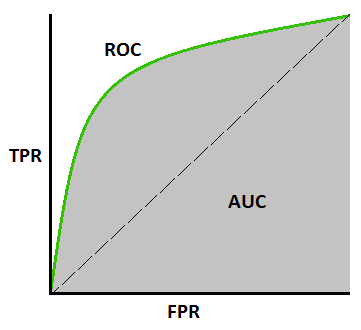
\includegraphics[width=0.65\textwidth, frame]{imagenes/Cap4/auc_roc}
  \caption{Ejemplo de un curva AUC-ROC \protect\cite{Reference62}.}
  \label{fig:auc_roc}
  \end{center}
\end{figure}


\vspace{5mm} %5mm vertical space

Existen dos razones principales por lo que se necesita esta curva, la primera es que refleja que tan bueno es el modelo para separar dos clases y la segunda es que ayuda a elegir el mejor umbral; por ejemplo, un AUC igual a 0,5 significa que el modelo separa dos posibles resultados al azar y un AUC de 1 (valor m\'{a}ximo) implica una separaci\'{o}n perfecta; por lo tanto se puede decir que mientras mayor sea el valor de AUC mejor es el rendimiento del modelo que se est\'{e} evaluando.

\subsection{F1 Score}

F1 Score define que tan preciso es un modelo, es decir, cu\'{a}ntas instancias clasifica correctamente, as\'{i} como tambi\'{e}n indica que tan robusto es el modelo. Esta m\'{e}trica es necesaria cuando se desea buscar un equilibrio entre la precisi\'{o}n y la recuperaci\'{o}n, ya que da una evaluaci\'{o}n justa incluso cuando el conjunto de datos se encuentra desequilibrado.

\subsubsection{Precisi\'{o}n (Precision)}

La precisi\'{o}n es el n\'{u}mero de resultados positivos correctos dividido por el n\'{u}mero de resultados positivos predichos por el clasificador.

\begin{equation}
Precision = \frac{VP}{VP+FP}
\end{equation}

\subsubsection{Recuperaci\'{o}n (Recall)}

Es el n\'{u}mero de resultados positivos correctos dividido por el n\'{u}mero de todas las muestras que deber\'{i}an haber sido clasificadas como positivas.

\begin{equation}
Recall = TPR = \frac{VP}{VP+FN}
\end{equation}

Por lo tanto, F1 Score se expresa matem\'{a}ticamente como:

\begin{equation}
F1 = 2*\frac{1}{\frac{1}{Precision}+\frac{1}{Recall}}
\end{equation}

%\section{Resumen del cap\'{i}tulo}

%Este cap\'{i}tulo detalla las bases te\'{o}ricas, permitiendo complementar los conocimientos necesarios para abordar el desarrollo del m\'{e}todo de detecci\'{o}n de anomal\'{i}as de conducci\'{o}n mediante el uso de Aprendizaje Autom\'{a}tico. En primer lugar, se decribi\'{o} los diferentes paradigmas de aprendizaje que existen y los diferentes enfoques de modelos, luego, se realiz\'{o} una descripci\'{o}n del funcionamiento de las redes neuronales y se mostr\'{o} sus diferentes tipos, as\'{i} como tambi\'{e}n diferentes t\'{e}cnicas de detecci\'{o}n de anomal\'{i}as y por \'{u}timo se presenta diferentes m\'{e}tricas de evaluaci\'{o}n de modelos de aprendizaje autom\'{a}tico. 

%El siguiente cap\'{i}tulo detalla el proceso de captura y preparaci\'{o}n del conjunto de datos, una etapa importante, debido a que este conjunto ser\'{a} aquel con el que se entrenar\'{a} el mecanismo de detecci\'{o}n de anomal\'{i}as propuesto.

El siguiente cap\'{i}tulo detalla el proceso de captura y preparaci\'{o}n del conjunto de datos, una etapa importante, debido a que este conjunto ser\'{a} aquel con el que se entrenar\'{a} el mecanismo de detecci\'{o}n de anomal\'{i}as propuesto.

% Chapter 3

\chapter{Captura y an\'{a}lisis de datos}
\label{Capitulo 3}

Contar con una gran cantidad de datos en cualquier problema de detecci\'{o}n de anomal\'{i}as es lo que permite generar modelos m\'{a}s precisos, debido a que nunca se sabe qu\'{e} caracter\'{i}sticas pueden dar indicio de una anomal\'{i}a, contar con m\'{u}ltiples tipos de datos es lo que permite ir m\'{a}s all\'{a} de una mera detecci\'{o}n de anomal\'{i}as puntuales y ser capaz de identificar anomal\'{i}as contextuales o colectivas m\'{a}s sofisticadas. Sin embargo la obtenci\'{o}n de estos datos no siempre es una tarea sencilla, por lo que muchas veces se debe encontrar una manera de generar los mismos.

\vspace{5mm} %5mm vertical space

En este cap\'{i}tulo se detallar\'{a} el m\'{e}todo de recolecci\'{o}n de datos que se realizar\'{a} para la presente investigaci\'{o}n y las diferentes t\'{e}cnicas de an\'{a}lisis de datos que se aplicar\'{a}.

\section{Captura de datos} \label{cap:CapDatos}

Actualmente existen varios enfoques para acceder a la información del conductor y del vehículo. En el primer enfoque, un conjunto de sensores y hardware adicional se implementan previamente en el veh\'{i}culo, por ejemplo, cajas telemáticas (cajas negras provistas por compañías de seguros de automóviles), adaptadores de diagnóstico a bordo (OBD-II) enchufados en el controlador del vehículo red de área (CAN) (\cite{30}, \cite{31}), la información registrada por estos dispositivos se puede recuperar o enviar a través de Internet. Sin embargo, esta estrategia requiere que los vehículos instalen dispositivos adicionales, lo que implica un mayor costo. Para superar estos inconvenientes, existe un enfoque alternativo el cual es usar teléfonos inteligentes para recopilar datos a través de un conjunto de sensores integrados, tales como sensores inerciales (acelerómetros y giroscopios), sistemas de posicionamiento global (GPS), magnetómetros, micrófonos, sensores de imagen (cámaras), sensores de luz , sensores de proximidad, sensores de dirección (brújula), entre otros.

\vspace{5mm} %5mm vertical space

Para el presente trabajo de grado se eligi\'{o} el uso de tel\'{e}fonos inteligentes para acceder a la informaci\'{o}n del tipo de conducci\'{o}n, por las razones que se presentaron anteriormente, con este enfoque se desarroll\'{o} una aplicaci\'{o}n m\'{o}vil basada en Android para recopilar datos de los sensores: aceler\'{o}metro y giroscopio, en intervalos de 1 segundo, los cuales en una primera instancia ser\'{a}n almacenados de manera interna en el dispositivo m\'{o}vil. (Ver Figura \ref{fig:captura})


\vspace{5mm} %5mm vertical space

\begin{figure}[h!]
  \begin{center}	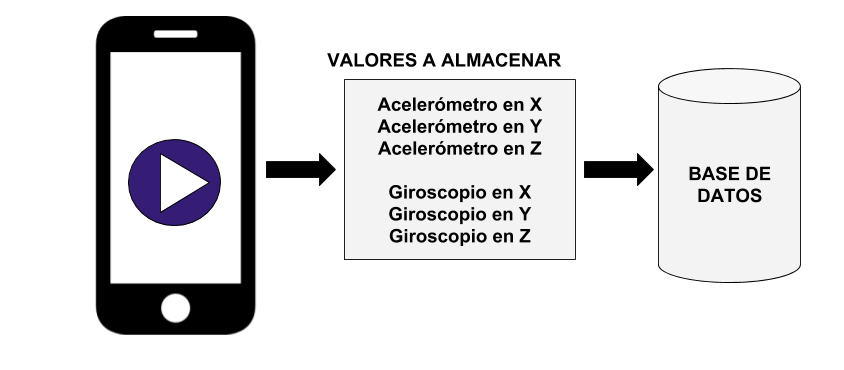
\includegraphics[width=0.95\textwidth]{imagenes/Cap3/captura}
  \caption{Recolecci\'{o}n de datos, con intervalo de un segundo.}
  \label{fig:captura}
  \end{center}
\end{figure}


\vspace{5mm} %5mm vertical space

Para la captura de datos se us\'{o} un soporte para celular de parabrisas como se ve en la Figura \ref{fig:soporte}; se realiz\'{o} la captura en dos posiciones distintas (vertical y horizontal).
\vspace{5mm} %5mm vertical space

\begin{figure}[h!]
  \begin{center}	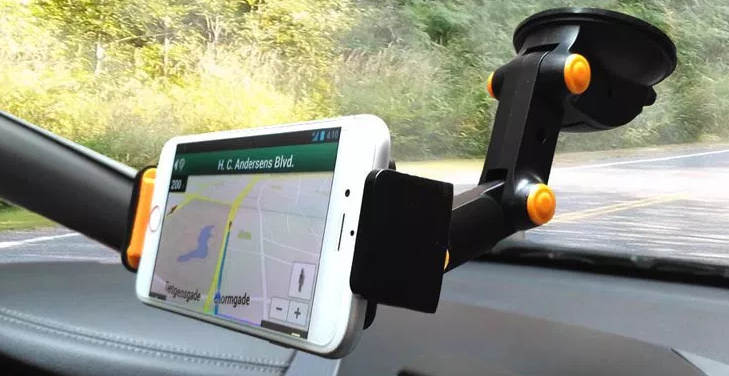
\includegraphics[width=0.65\textwidth]{imagenes/Cap3/soporte}
  \caption{Soporte para celular de parabrisas, posici\'{o}n horizontal.}
  \label{fig:soporte}
  \end{center}
\end{figure}

Cada captura, independientemente de la posici\'{o}n en la que se realiz\'{o}, di\'{o} como resultado un conjunto de datos (dataset), donde por cada tiempo T (1 seg.) se tiene seis variables: aceler\'{o}metro en X (acc x), aceler\'{o}metro en Y (acc y), aceler\'{o}metro en Z (acc z), giroscopio en X (gyr x), giroscopio en Y (gyr y) y giroscopio en Z (gyr z). En la Figura \ref{fig:dataset} se aprecia un fragmento del conjunto de datos que se obtuvo en una captura.

\begin{figure}[h!]
  \begin{center}	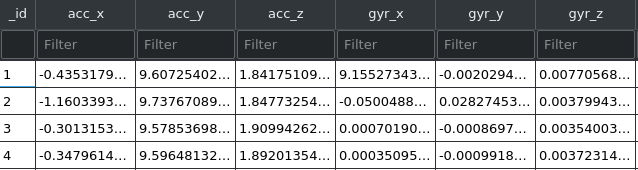
\includegraphics[width=0.95\textwidth]{imagenes/Cap3/dataset}
  \caption{Fragmento del conjunto de datos obtenido.}
  \label{fig:dataset}
  \end{center}
\end{figure}

\section{Preparaci\'{o}n de datos}

El Aprendizaje Autom\'{a}tico depende en gran medida de los datos. Son el aspecto m\'{a}s crucial que hace posible el entrenamiento de algoritmos y explica porque el aprendizaje autom\'{a}tico se hizo tan popular en los \'{u}ltimos a\~{n}os. El principal problema es que todos los conjuntos de datos tienen fallas, lo que hace a la preparaci\'{o}n de datos un paso muy importante en el proceso de Aprendizaje Autom\'{a}tico.

\vspace{5mm} %5mm vertical space

El prop\'{o}sito principal de la preparaci\'{o}n de datos es manipular y transformar los datos en crudo, tal que, los datos puedan ser expuestos o hacerse accesibles m\'{a}s facilmente \cite{37}, para lograr este prop\'{o}sito se debe seguir un proceso que implica la selecci\'{o}n, el pre-procesamiento y la transformaci\'{o}n de datos.
 
\subsection{Selecci\'{o}n de datos}

La selecc\'{o}n de datos implica los siguientes pasos:

\begin{itemize}
\item Seleccionar solo un subconjunto de los datos disponibles.
\item Derivar o simular algunos datos a partir de los datos diponibles, en caso de ser necesario.
\item Excluir aquellos datos que no son reelevantes para el problema.
\end{itemize}

Para el presente trabajo se har\'{a} incapi\'{e} s\'{o}lo en el primer paso de esta fase, debido a que los datos con los que se cuenta son limitados ya que \'{e}stos fueron capturados para la investigaci\'{o}n y como se indic\'{o} en la secci\'{o}n \ref{cap:CapDatos}, esta captura se realiz\'{o}, tanto de forma vertical como horizontal, a continuaci\'{o}n se analizar\'{a} las diferencias entre ellos.

\vspace{5mm} %5mm vertical space

En la Figura \ref{fig:verHor} se muestra fragmentos de las capturas obtenidas por el dispositivo m\'{o}vil del manejo de un mismo usuario desde diferentes posiciones.

\begin{figure}
        \centering
        \begin{subfigure}[h]{0.47\textwidth} 
            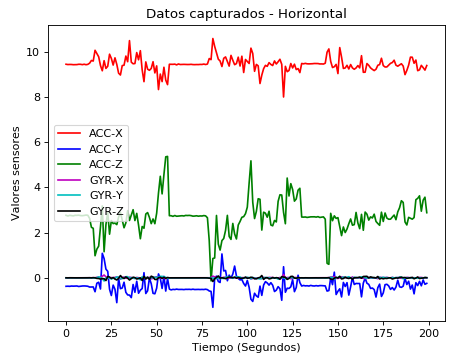
\includegraphics[width=\textwidth]{imagenes/Cap3/horizontal}
            \caption{Captura de datos en horizontal}
            \label{fig:hor}
        \end{subfigure}       
        \begin{subfigure}[h]{0.47\textwidth} 
            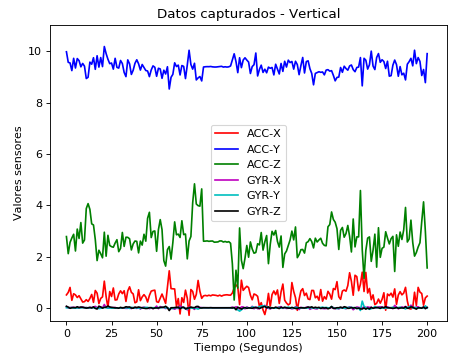
\includegraphics[width=\textwidth]{imagenes/Cap3/vertical}
            \caption{Captura de datos en vertical}
            \label{fig:ver}
        \end{subfigure}
        \caption{Gr\'{a}fica de los sensores capturados en diferentes posiciones}
        		\label{fig:verHor}
    \end{figure}

\vspace{5mm} %5mm vertical space

Si bien los valores capturados, son muy similares entre s\'{i}, los datos que fueron capturados con el dispositivo m\'{o}vil en posici\'{o}n horizontal, presentan menos ruido, esto debido a que esta posici\'{o}n favorece la inercia del dispositivo cuando el veh\'{i}culo est\'{a} en movimiento, lo cual es una gran ventaja frente a los datos que fueron capturados de forma vertical, ya que estos fueron m\'{a}s suceptibles a sacudirse mientras el veh\'{i}culo se desplazaba haciendo que los valores capturados en esta posici\'{o}n presenten valores de movimiento no s\'{o}lo del veh\'{i}culo sino tambi\'{e}n del dispositivo m\'{o}vil, lo cual no es lo que se busca en el presente trabajo.

\vspace{5mm} %5mm vertical space

Por las razones presentadas en el anterior p\'{a}rrafo se decidi\'{o} trabajar con los datos capturados con el dispositivo m\'{o}vil en posici\'{o}n horizontal, descartando as\'{i} aquellos datos capturados en vertical.

\section{Pre-procesamiento de datos}

Una vez que se seleccionaron los datos con los que se trabajar\'{a}, se debe proceder a pre-procesarlos, entrando as\'{i} a la fase de Pre-procesamiento de datos, el objetivo de esta fase es reducir la cantidad de los datos, encontrar las relaciones entre ellos, normalizarlos, remover los valores at\'{i}picos y extraer las caracter\'{i}sticas de los datos. Esta fase incluye varias t\'{e}cnicas como la limpieza, integraci\'{o}n, transformaci\'{o}n y reduci\'{o}n de los datos \cite{38}.

\subsection{Limpieza de datos}

Los datos de las filas pueden tener registros incompletos, valores ruidosos, valores at\'{i}picos y datos inconsistentes. La limpieza de los datos en la mayor\'{i}a de los casos es el primer paso del pre-procesamiento de datos. Esta t\'{e}cnica se usa para encontrar valores ausentes, suavizar el ruido en los datos, reconocer valores at\'{i}picos y corregir inconsistencias.

\subsubsection{Manejo de valores ausentes}

Los valores ausentes en el conjunto de datos pueden ser llenados usando cualquiera de las t\'{e}cnicas que se mencionan a continuaci\'{o}n.

\begin{itemize}
\item \textbf{Ignorar / Eliminar:} En algunos casos es mejor ignorar o eliminar la tupla que contiene valores faltantes en lugar de llenar esta. Generalmente esta t\'{e}cnica se practica en conjuntos de datos que son muy grandes, donde el eliminar algunos datos no afectara la informaci\'{o}n que transmite nuestro conjunto de datos. Sin embargo cuando se trabaja con un conjunto de datos peque\~{n}o el eliminar las tuplas que contienen valores ausentes podr\'{i}a hacer perder informaci\'{o}n importante.

\item \textbf{Llenar manualmente los valores ausentes:} Otra opci\'{o}n tambi\'{e}n es completar los valores faltantes si se comprende la naturaleza de los mismos, esto generalmente se realiza en conjunto de datos peque\~{n}os, ya que en los conjuntos grandes esta tarea requerir\'{i}a bastante tiempo.

\item \textbf{Llenar los valores ausentes con valores centrales (Media/Mediana):} Esta t\'{e}cnica es mucho mejor que las presentadas anteriormente. En esta t\'{e}cnica se inserta la media o la mediana del atributo respectivo a los valores faltantes. 

\item \textbf{Interpolaci\'{o}n:} Es una forma confiable, precisa y cient\'{i}fica de completar valores perdidos. Para usar esta t\'{e}cnica primero se debe desarrollar una relaci\'{o}n entre los atributos y luego se predice el valor mas probable y preciso para los lugares faltantes, esto se puede lograr mediante regresi\'{o}n, formulaci\'{o}n bayesiana e inducci\'{o}n por \'{a}rboles de decisi\'{o}n.

\end{itemize}

\subsubsection{Eliminar rudio (suavizado) de los datos}

Para comprender esta t\'{e}cnica primero se debe definir qu\'{e} es el ruido en los datos. El ruido en los datos es cualquier tipo de error aleatorio o variaci\'{o}n en los atributos medidos; por otra parte los valores at\'{i}picos presentes en los datos tambi\'{e}n pueden considerarse como ruido. 

\vspace{5mm} %5mm vertical space

Es importante destacar que el ruido presente en el conjunto de datos puede afectar en gran medida el resultado de nuestros algoritmos de Aprendizaje Autom\'{a}tico, por lo tanto aquellos datos que contengan ruido no son considerados buenos datos y deben ser eliminados en lo posible. Sin embargo antes de eliminar estos, se debe ser capaz de detectarlos; para lograr este objetivo existen muchas t\'{e}cnicas que se pueden utilizar, una de estas t\'{e}cnicas es la \textbf{Visualizaci\'{o}n de datos}, la cual consiste en obtener una representaci\'{o}n visual de nuestros datos, para poder evidenciar si existe ruido en los datos y/o valores at\'{i}picos.

\vspace{5mm} %5mm vertical space

En el presente proyecto se grafic\'{o} histogramas de las frecuencias de cada caracter\'{i}stica de nuestro conjunto de datos y as\'{i} visualizar de mejor manera si existe ruido o valores at\'{i}picos en el mismo. En la Figura \ref{fig:hist} se puede evidenciar que los valores de cada sensor presentan asimetr\'{i}as negativas y positivas, adem\'{a}s de tener muchos valores bastante alejados de la media, lo que d\'{a} un indicio de posibles valores at\'{i}picos.

\begin{figure}[h!]
  \begin{center}	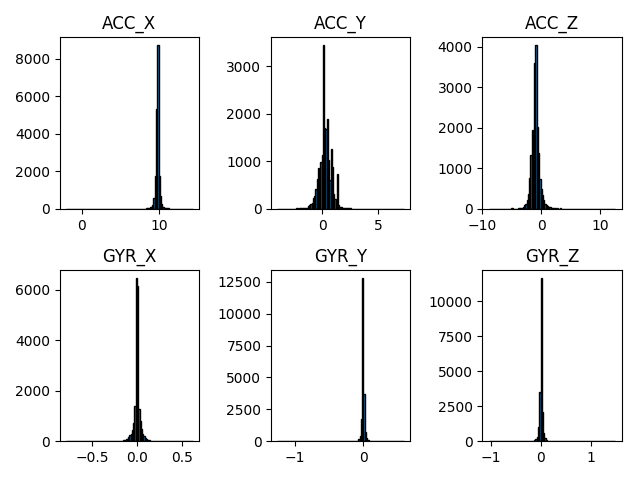
\includegraphics[width=0.97\textwidth]{imagenes/Cap3/histograma_sensores}
  \caption{Histograma de frecuencias del conjunto de datos}
  \label{fig:hist}
  \end{center}
\end{figure}

\vspace{5mm} %5mm vertical space

En la Figura \ref{tab: est} se presenta una tabla con estad\'{i}sticas descriptivas de nuestro conjunto de datos, esta tabla presenta: la cantidad de datos, su media, su desviaci\'{o}n est\'{a}ndar, el valor m\'{i}nimo y m\'{a}ximo del conjunto de datos y los percentiles 50, 25 y 75, cabe recalcar que el percentil 50 es el mismo que la mediana.

\begin{figure}[h!]
  \begin{center}	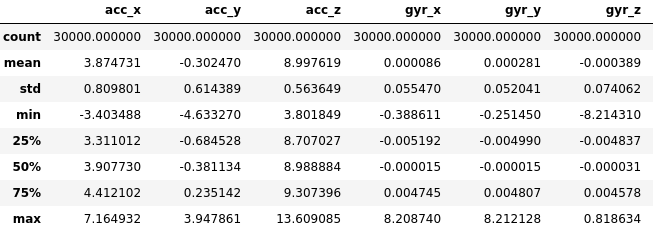
\includegraphics[width=0.97\textwidth]{imagenes/Cap3/describe_data}
  \caption{Tabla de resultados estad\'{i}sticos del conjunto de datos.}
  \label{tab: est}
  \end{center}
\end{figure}

\vspace{5mm} %5mm vertical space

Con la informaci\'{o}n proporcionada en la Figura \ref{tab: est} ahora es m\'{a}s sencillo realizar un an\'{a}lisis del conjunto de datos, en primer lugar se evidencia que los valores obtenidos durante la captura, presentan desviaciones est\'{a}ndar muy peque\~{n}as entre 0.02 y 0.79 y sin embargo la diferencia entre los valores m\'{i}nimo y m\'{a}ximo son realmente grandes, por ejemplo para el Aceler\'{o}metro en X, la diferencia es 16 aproximadamente (Valor m\'{i}nimo: -1.998 y valor m\'{a}ximo: 14.31), esto quiere decir que nuestro conjunto de datos presenta mucho ruido, considerando como ruido o valores at\'{i}picos, aquellos valores muy alejados de la media. 

\vspace{5mm} %5mm vertical space

Para eliminar el ruido que presenta nuestro conjunto de datos se aplic\'{o} la \textbf{Regla 68-95-99.7}, conocida tambi\'{e}n como la \textbf{Regla emp\'{i}rica}, donde suponiendo que el conjunto de datos con el que se trabaja tiene una distribuci\'{o}n normal, la desviaci\'{o}n est\'{a}ndar se puede usar para determinar la proporci\'{o}n de valores que se encuentran dentro de un rango particular del valor medio. Para tales distribuciones, siempre ocurre que el 68\% de los valores est\'{a}n a menos de una desviaci\'{o}n est\'{a}ndar (1SD) del valor medio, que el 95\% de los valores est\'{a}n a menos de dos desviaciones est\'{a}ndar (2SD) de la media y que el 99\% de valores est\'{a}n a menos de tres desviaciones est\'{a}ndar (3SD) de la media. En la Figura \ref{fig:689599rule} se muestra este concepto de forma esquem\'{a}tica.

\begin{figure}[h!]
  \begin{center}	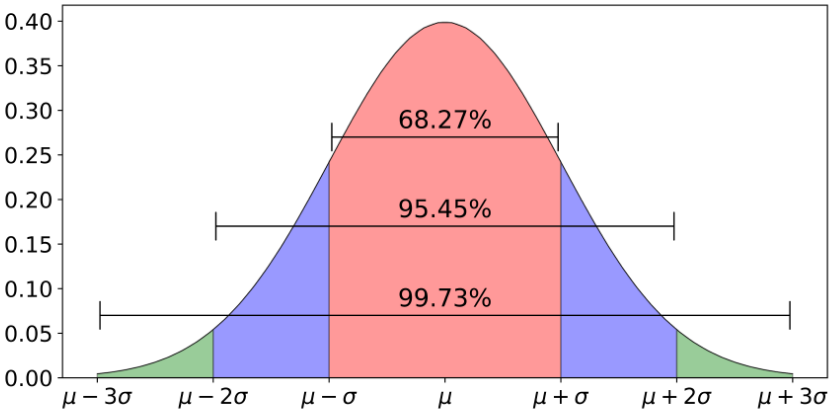
\includegraphics[width=0.97\textwidth]{imagenes/Cap3/68-95-99_rule}
  \caption{Regla 68-95-99.7 }
  \label{fig:689599rule}
  \end{center}
\end{figure}

En la Figura \ref{fig:689599rule_acc_y}, se puede observar como se comporta la regla 68-95-99.7 sobre los valores del sensor del aceler\'{o}metro en Y, por lo que para eliminar el ruido en nuestro conjunto de datos se tiene dos opciones, eliminar los valores despu\'{e}s de tres desviaciones est\'{a}ndar de la media, en caso de considerar que nuestro conjunto de datos presenta pocas anomal\'{i}as o valores at\'{i}picos, o eliminar los valores despu\'{e}s de dos desviaciones est\'{a}ndar en caso de estar seguro que nuestro conjunto de datos presenta una gran cantidad de ruido en los datos, en nuestro caso la mayor\'{i}a de nuestros datos pertenecen a comportamientos normales de conducci\'{o}n por lo que s\'{o}lo eliminaremos los valores que se encuentran despu\'{e}s de tres desviaciones est\'{a}ndar de la media.


\begin{figure}[h!]
  \begin{center}	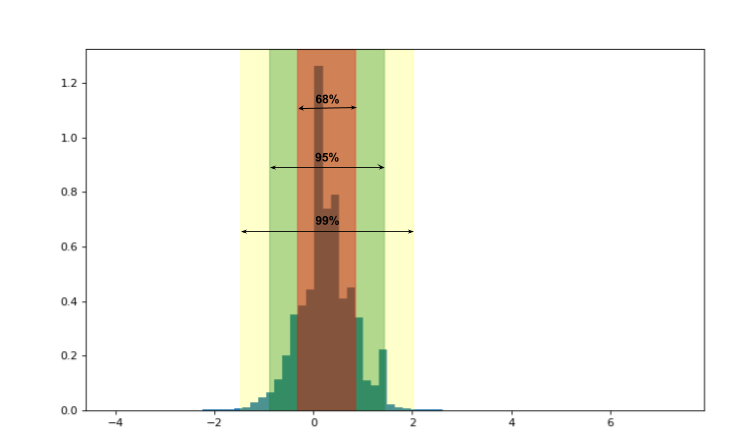
\includegraphics[width=0.97\textwidth]{imagenes/Cap3/acc_y_689599_rule}
  \caption{Regla 68-95-99.7 aplicada a los valores de los sensores del aceler\'{o}metro en Y. }
  \label{fig:689599rule_acc_y}
  \end{center}
\end{figure}

\subsubsection{Fusi\'{o}n o integraci\'{o}n de datos}

Cuando se trabaja con datos del mundo real, es posible que los datos que se requiere no se encuentren en un mismo conjunto de datos, en \'{e}stos casos, se necesita recopilar datos de diferentes fuentes y fusionarlos en un solo conjunto de datos; este proceso recibe el nombre de Fusi\'{o}n o Integraci\'{o}n de datos. Uno de los problemas m\'{a}s comunes de este proceso es la redundancia. 

\vspace{5mm} %5mm vertical space

Este proceso no se aplic\'{o} en la investigaci\'{o}n debido a que s\'{o}lo se capturo los datos por medio del dispositivo m\'{o}vil, por lo cual no se tiene el problema de tener m\'{a}s de una fuente de datos.

\subsubsection{Transformaci\'{o}n de datos}
\label{subsubsection:est-norm-dataset}

La transformaci\'{o}n de los datos es el proceso donde se cambia la naturaleza de los datos, dicho proceso usa algunas estrategias para poder extraer informaci\'{o}n importante del conjunto de datos; algunas de las estrategias para la transformaci\'{o}n de datos son: 

\begin{itemize}
\item \textbf{Agregaci\'{o}n: }En esta t\'{e}cnica, la operaci\'{o}n de resumen o agregaci\'{o}n se aplica sobre los datos. Por ejemplo: los datos de ventas diarias se pueden usar para calcular el monto mensual y anual en ventas, para posteriormente agregar estos datos calculados al conjunto de datos.

\item \textbf{Discretizaci\'{o}n: }Con esta t\'{e}cnica se construye y reemplaza valores en bruto de un atributo num\'{e}rico por valores de intervalo.

\item \textbf{Construcci\'{o}n de atributos / Ingenier\'{i}a de caracter\'{i}sticas: }Esta t\'{e}cnica es \'{u}til para generar informaci\'{o}n adicional a partir de datos vagos, adem\'{a}s puede ser adecuada cuando se tiene menos caracter\'{i}sticas pero a\'{u}n contienen informaci\'{o}n oculta para extraer.

\item \textbf{Normalizaci\'{o}n / Estandarizaci\'{o}n: }La normalizaci\'{o}n o estandarizaci\'{o}n se define como el proceso de reescalar datos originales sin cambiar su comportamiento o naturaleza. Se define un nuevo l\'{i}mite (generalmente entre 0 y 1) y se convierte los datos en consecuencia. Esta t\'{e}cnica es \'{u}til en algoritmos de clasificaci\'{o}n que involucran redes neuronales o algoritmos basados en la distancia (por ejemplo, KNN, K-means). Algunas t\'{e}cnicas de normalizaci\'{o}n son:
\begin{itemize}
\item \textit{Normalizaci\'{o}n Min-Max: }En este m\'{e}todo, cada entrada se normaliza entre unos l\'{i}mites definidos:

\begin{equation}
x_{normalizado} = \frac{x - x_{min}}{x_{max}-x_{min}}
\end{equation}

Presenta el problema de que comprime los datos de entrada entre unos límites fijos, que por lo general son 0 y 1. Esto quiere decir que si existe ruido, éste va a ser ampliado, lo que hace que este m\'{e}todo no sea adecuado para señales estables.

\item \textit{Escalado est\'{a}ndar (Standard Scaler): }Es un m\'{e}todo alternativo al escalado de variables, consiste en restar a cada dato la media de la variable y dividirlo por la desviaci\'{o}n t\'{i}pica.

\begin{equation}
x_{normalizado} = \frac{x - x_{media}}{x_{desvSt}}
\end{equation}

\'{E}ste m\'{e}todo es adecuado para normalizar se\~{n}ales estables, no obstante, tanto la media como la desviaci\'{o}n est\'{a}ndar son muy sensibles a valores an\'{o}malos. Una alternativa de soluci\'{o}n de esto es la eliminaci\'{o}n de anomal\'{i}as antes de realizar la normalizaci\'{o}n.

\item \textit{Escalado sobre el valor m\'{a}ximo: }Este m\'{e}todo, presenta la idea de escalar los datos dividiendo \'{e}stos entre su m\'{a}ximo valor.

\item \textit{Escalado robusto (Robust scaler): }El escalado robusto consiste en eliminar la mediana y escala los datos de acuerdo con el rango de interquartil (IQR). Este m\'{e}todo es robusto para valores at\'{i}picos.

\end{itemize}

\end{itemize}

\subsubsection{Reducci\'{o}n de datos}

Este proceso se basa en la adopci\'{o}n de algunas estrategias, tal que el an\'{a}lisis de datos reducidos produce la misma informaci\'{o}n producida por los datos originales. Algunas de las estrategias incluyen: an\'{a}lisis de componentes principales (PCA), selecci\'{o}n de un subconjunto de atributos, agrupaci\'{o}n y muestreo entre otros.

\vspace{5mm} %5mm vertical space

\textbf{An\'{a}lisis de componentes principales (PCA)}

\vspace{5mm} %5mm vertical space

El An\'{a}lisis de Componentes Principales (PCA - Principal Component Analysis) es una técnica que se usa ampliamente para aplicaciones como reducción de dimensionalidad, compresión de datos con pérdida, extracción de características y visualización de datos \cite{39}.

\vspace{5mm} %5mm vertical space

PCA es una t\'{e}cnica estad\'{i}stica no supervisada y no param\'{e}trica, que se utiliza para la reducci\'{o}n de dimensionalidad. Esta t\'{e}cnica es un paso importante debido a que la alta dimensionalidad en el campo de aprendizaje autom\'{a}tico puede llevar al sobreajuste del modelo, reduciendo as\'{i} su capacidad de generalizaci\'{o}n, Richard Bellman en \cite{40} describe este fen\'{o}meno como la "Maldici\'{o}n de la Dimensionalidad". Adem\'{a}s, el uso de esta t\'{e}cnica puede mejorar directamente el rendimiento de los modelos de Aprendizaje Autom\'{a}tico.

\vspace{5mm} %5mm vertical space

PCA combina las variables de entrada de una manera espec\'{i}fica, luego se deshace de las variables "menos importantes" y al mismo tiempo conserva las partes m\'{a}s valiosas (o componentes principales\footnote{\textbf{Componente principal}, es una combinaci\'{o}n lineal normalizada de las caracter\'{i}sticas originales en el conjunto de datos.}) de todas las variables.

\vspace{5mm} %5mm vertical space

Cuando se usa PCA enfocado al aprendizaje autom\'{a}tico se sigue los siguientes pasos:

\begin{enumerate}

\item Dividir el conjunto de datos \textit{d}-dimensional en conjunto de entrenamiendo, desarrollo y prueba.
\item Estandarizar / Normalizar el conjunto de datos seg\'{u}n el conjunto de entrenamiento.
\item Construir la matriz de covarianza.
\item Descomponer la matriz de covarianza en sus vectores y valores propios.
\item Ordenar los valores propios disminuyendo el orden para clasificar los vectores propios correspondientes.
\item Seleccionar \textit{k} vectores propios que corresponden a los \textit{k} valores propios m\'{a}s grandes, donde \textit{k} es la dimensionalidad del nuevo subespacio de entidad (\textit{k}<=\textit{d}).
\item Construir una matriz de proyecci\'{o}n \textbf{W} a partir de los "top" \textit{k} vectores propios.
\item Transformar el conjunto de entrenamiento de entrada \textit{d}-dimensional \textbf{X} utilizando la matriz de proyecci\'{o}n \textbf{W} para obtener el nuevo subespacio de caracter\'{i}stica \textit{k}-dimensional.

\end{enumerate}

\vspace{5mm} %5mm vertical space

\textbf{\textit{Dividir el conjunto de datos}}

\vspace{5mm} %5mm vertical space

Dado que se cuenta con un conjunto de datos para generar el modelo de Aprendizaje Autom\'{a}tico, este se divide en tres partes: conjunto de entrenamiento\footnote{\textbf{Conjunto de entrenamiento}, es la muestra de datos utilizada para ajustar el modelo de Aprendizaje Autom\'{a}tico.}, desarrollo\footnote{\textbf{Conjunto de desarrollo}, es la muestra de datos utilizada para proporcionar una evaluaci\'{o}n imparcial de un modelo ajustado con el conjunto de entrenamiento mientras se ajustan los hiperpar\'{a}metros del modelo.} y prueba\footnote{\textbf{Conjunto de prueba}, es la muestra de datos utilizada para proporcionar una evaluaci\'{o}n imparcial de un ajuste final del modelo en el conjunto de entrenamiento.}, sin embargo esto no es una tarea trivial; ya que si no se hace correctamente el resultado puede ser desastroso.

\vspace{5mm} %5mm vertical space

\begin{figure}[h!]
  \begin{center}	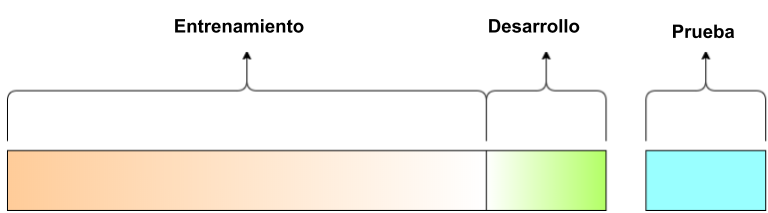
\includegraphics[width=0.97\textwidth]{imagenes/Cap3/train-dev-test}
  \caption{Divisi\'{o}n del conjunto de entrenamiento.}
  \label{fig:train-dev-test}
  \end{center}
\end{figure}

En \cite{42} se dice que la divisi\'{o}n del conjunto de datos tiene un gran impacto en la productividad , por lo cual es importante que al elegir todos nuestros subconjuntos estos deben tener la \textbf{misma distribuci\'{o}n} y deben ser elegidos aleatoriamente del conjunto de datos. 

\vspace{5mm} %5mm vertical space

Por otra parte el tama\~{n}o del conjunto de desarrollo y prueba deben ser lo suficientemente grandes como para que los resultados del desarrollo y prueba sean representativos para el rendimiento del modelo. Para conjuntos de datos grandes (mayores a un mill\'{o}n), el conjunto de desarrollo y prueba puede tener alrededor de 10000 ejemplos cada uno, es decir, el 1\% del total de datos.

\vspace{5mm} %5mm vertical space

Otras consideraciones que deben tomarse en cuenta en la pr\'{a}ctica son:

\begin{itemize}
\item La divisi\'{o}n del conjunto de entrenamiento/desarrollo/prueba siempre debe ser la misma para todos los experimentos, por lo tanto se debe contar con script reproducible para crear la divisi\'{o}n entrenamiento/desarrollo/prueba.
\item Se debe probar que los conjuntos de desarrollo y prueba provengan de la misma distribuci\'{o}n.
\end{itemize}

En la presente investigaci\'{o}n nuestro conjunto de datos cuenta con 30000 ejemplos, por lo que la divisi\'{o}n de nuestro conjunto de datos ser\'{a} la que se observa en el Cuadro \ref{table:division-dataset}.


\begin{table}[]
\centering
\begin{tabular}{|l|l|l|}
\hline
Conjunto de entrenamiento & 70\%  & 21000 \\ \hline
Conjunto de desarrollo    & 15\%  & 4500  \\ \hline
Conjunto de prueba        & 15\%  & 4500  \\ \hline
Conjunto de datos         & 100\% & 30000 \\ \hline
\end{tabular}
\caption{Tabla de divisi\'{o}n del conjunto de datos.}
\label{table:division-dataset}
\end{table}

\vspace{5mm} %5mm vertical space

\textbf{\textit{Estandarizar / Normalizar el conjunto de datos}}

\vspace{5mm} %5mm vertical space

En la secci\'{o}n \ref{subsubsection:est-norm-dataset} ya se describi\'{o} lo que es la estandarizaci\'{o}n o normalizaci\'{o}n de datos y algunos de los tipos de escalado que existen; por lo tanto esta secci\'{o}n s\'{o}lo se limitar\'{a} a la elaboraci\'{o}n de un an\'{a}lisis para decidir que t\'{e}cnica de escalado es la m\'{a}s adecuada para el conjunto de datos, en la Figura \ref{fig:datos_puros} se puede apreciar una fracci\'{o}n del conjunto de datos capturado, la cual es la base con la que se realizar\'{a} el an\'{a}lisis comparativo con los distintos tipos de escalado.

\begin{figure}[h!]
  \begin{center}	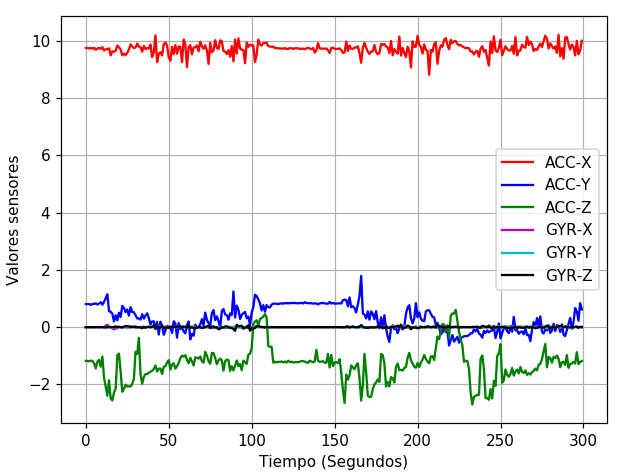
\includegraphics[width=0.5\textwidth]{imagenes/Cap3/datos_sin_preprocesamiento}
  \caption{Visualizaci\'{o}n de los par\'{a}metros de conducci\'{o}n capturados.}
  \label{fig:datos_puros}
  \end{center}
\end{figure}

\vspace{5mm} %5mm vertical space

Para probar los diferentes tipos de escalado, se los ajusto con los datos que ya no presentan ruido o valores at\'{i}picos del conjunto de entrenamiento.

\begin{figure}
        \centering
        \begin{subfigure}[h]{0.45\textwidth} 
            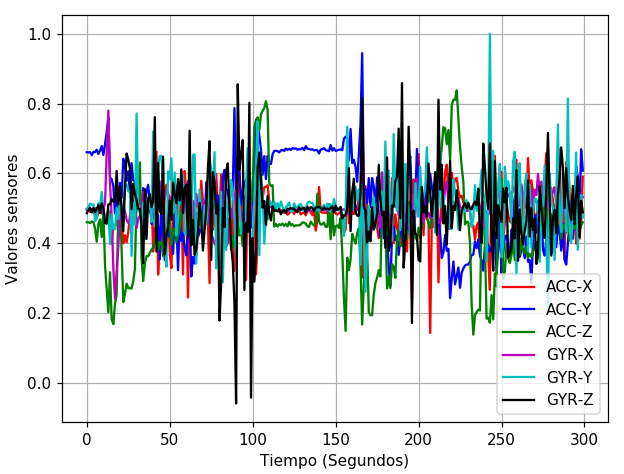
\includegraphics[width=\textwidth]{imagenes/Cap3/datos_minmax_scaler}
            \caption{Min max Scaler}
            \label{fig:min_max}
        \end{subfigure}       
        \begin{subfigure}[h]{0.45\textwidth} 
            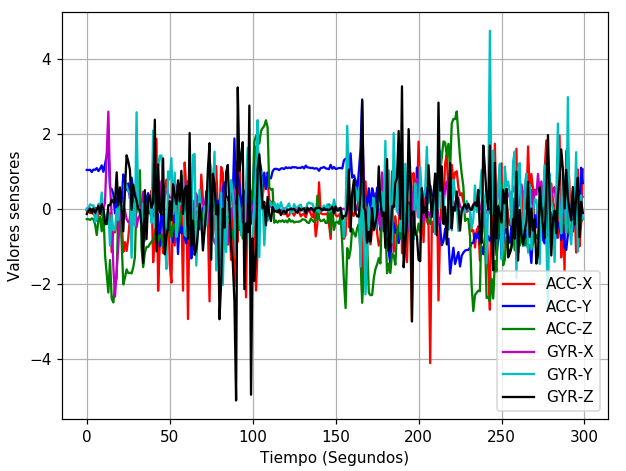
\includegraphics[width=\textwidth]{imagenes/Cap3/datos_standard_scaler}
            \caption{Standard Scaler}
            \label{fig:standard}
        \end{subfigure}
        
        \begin{subfigure}[h]{0.45\textwidth} 
            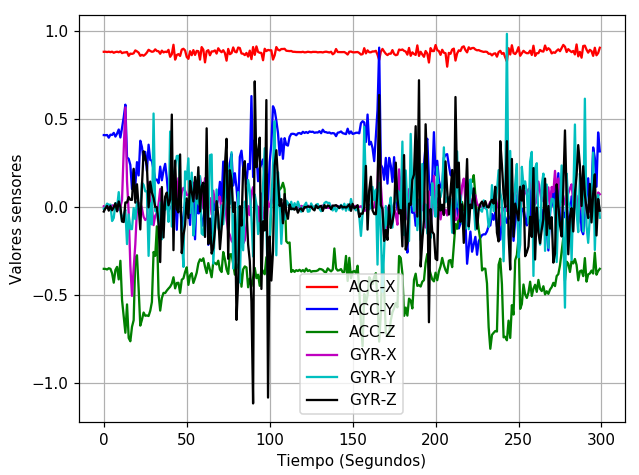
\includegraphics[width=\textwidth]{imagenes/Cap3/datos_max_scaler}
            \caption{Max Scaler}
            \label{fig:max}
        \end{subfigure}       
        \begin{subfigure}[h]{0.45\textwidth} 
            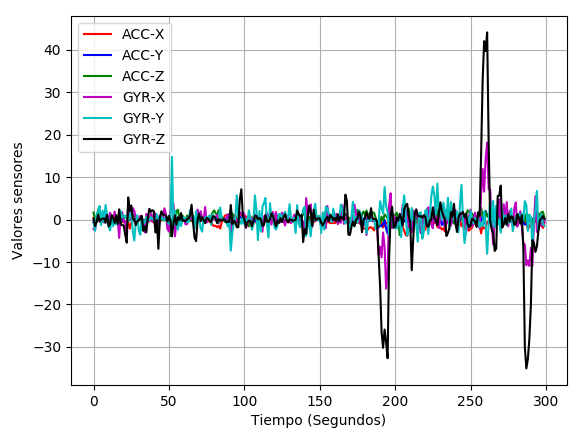
\includegraphics[width=\textwidth]{imagenes/Cap3/datos_robust_scaler}
            \caption{Robust Scaler}
            \label{fig:robust}
        \end{subfigure}
        \caption{Gr\'{a}fica resultante de aplicar diferentes tipos de normalizaciones a un conjunto de datos.}
        
		\label{fig:nor_nor}
    \end{figure}

\vspace{5mm} %5mm vertical space

El primer tipo de escalado que se realiz\'{o} sobre el conjunto de datos capturados fue la \textbf{Normalizaci\'{o}n Min-Max}, el cual se realiz\'{o} entre los l\'{i}mites 0 y 1, los resultados obtenidos se muestran en la figura \ref{fig:min_max}, donde se puede apreciar que los valores del aceler\'{o}metro, en sus tres ejes, no se veen deformados despu\'{e}s de haber sido escalados con \'{e}sta t\'{e}cnica y los valores del giroscopio, los cuales son m\'{a}s estables se tornan deformados, considerando como datos estables aquellos datos que se presentan como una l\'{i}nea en cero con pocas fluctuaciones; esta deformaci\'{o}n puede ser ventajosa al hacer m\'{a}s visible peque\~{n}as curvas que anteriormente eran imperceptibles, sin embargo conlleva el peligro de que pueda ampliar ruido existente en nuestros datos que no pudimos eliminar en el paso previo a esta tarea.


\vspace{5mm} %5mm vertical space

La segunda t\'{e}cnica de normalizaci\'{o}n que se aplic\'{o} sobre los datos fue el \textbf{escalado est\'{a}ndar}, el resultado se puede apreciar en la figura \ref{fig:standard}, observando detalladamente los resultados se puede evidenciar que son muy similares a los obtenidos con la normalizaci\'{o}n Min-Max, las \'{u}nicas diferencias que se pueden evidencias son que el nuevo rango de los datos es m\'{a}s amplio con media en cero y valores que oscilan principalmente entre 2 y 2,  y que se amplia un poco m\'{a}s algunas de las fluctuaciones que presentan los giroscopios.

\vspace{5mm} %5mm vertical space

Para la tercera normalizaci\'{o}n de datos se aplic\'{o} la t\'{e}cnica de \textbf{escalado sobre el valor m\'{a}ximo}, los resultados se presentan totalmente diferentes a los que seobtuvo anteriormente, sin embargo se observa claramente que los valores del aceler\'{o}metro no presentan mucho cambio con la diferencia de que la media de estos valores son distintas para cada uno, y los valores de los giroscopios se comportan como en los anteriores, como se puede ver en la figura \ref{fig:max}. Esta t\'{e}cnica presenta los peores resultados, ya que no deja nuestro conjunto de datos en un mismo rango lo cual complica su trabajo.

\vspace{5mm} %5mm vertical space

La \'{u}ltima t\'{e}cnica aplicada es el \textbf{escalado robusto}, su resultado puede ser observado en la figura \ref{fig:robust}, el cual puede ser considerado bastante similar a las dos primeras t\'{e}cnicas, con diferencia de que este escalado pronuncia mucho m\'{a}s las fluctuaciones de los valores de los giroscopios.

\vspace{5mm} %5mm vertical space

Para decidir el mejor m\'{e}todo de normalizaci\'{o}n que se puede aplicar a los datos capturados, primero se descartar\'{a} completamente el \textbf{m\'{e}todo de escalado sobre el valor m\'{a}ximo} debido a que los resultados que present\'{o} fueron totalmente desalentadores ya que los valores despu\'{e}s del escalado no compart\'{i}an los mismos l\'{i}mites, por otra parte los restantes tres tipos de escalado son muy similares, lo cual complica la elecci\'{o}n de escalado correcto, sin embargo cuando se usa PCA se debe ser muy cuidadoso, debido a que si se tiene una variable con una desviaci\'{o}n est\'{a}ndar alta, esta tendr\'{a} un mayor peso en el c\'{a}lculo del eje que una variable con una desviaci\'{o}n est\'{a}nda baja, por lo cual este puede ser un par\'{a}metro de decisi\'{o}n importante para elegir el tipo de escalado m\'{a}s adecuado.

\vspace{5mm} %5mm vertical space

En la tabla \ref{table:scalers} se muestra la media y la desviaci\'{o}n est\'{a}ndar de cada variable despu\'{e}s de haber aplicado los diferentes tipos de escalado sobre los datos. Como se puede evidenciar en los escalados sobre el valor m\'{a}ximo y est\'{a}ndar, las desviaciones est\'{a}ndar son muy diferentes, en cuanto al escalado Min-Max las desviaciones est\'{a}ndar de cada variable son casi las mismas todas oscilan entre 0.166759	 y 0.169528, lo cual se adec\'{u}a muy bien para el an\'{a}lisis de componentes principales, que es lo que se busca en este punto.


\begin{landscape}
\pagestyle{empty}
\begin{table}[p!]

\centering
\begin{tabular}{ll|r|r|r|r|r|r|}
\cline{3-8}
 &  & \multicolumn{1}{c|}{\textbf{ACC X}} & \multicolumn{1}{c|}{\textbf{ACC Y}} & \multicolumn{1}{c|}{\textbf{ACC Z}} & \multicolumn{1}{c|}{\textbf{GYR X}} & \multicolumn{1}{c|}{\textbf{GYR Y}} & \multicolumn{1}{c|}{\textbf{GYR Z}} \\ \hline
\multicolumn{1}{|l|}{\multirow{4}{*}{Min-Max}} & Media & 0.494631 & 0.504011 & 0.500105 & 0.497873 & 0.499490 & 0.499922 \\ \cline{2-8} 
\multicolumn{1}{|l|}{}                  & Desv. Est. & 0.169528 & 0.168058 & 0.166759 & 0.167592 & 0.167005 & 0.166876 \\ \cline{2-8} 
\multicolumn{1}{|l|}{}                  & M\'{i}nimo & -3.932480 & -0.736326	& -1.182118 & -2.239772 & -8.435568 & -3.984707 \\ \cline{2-8} 
\multicolumn{1}{|l|}{}                  & M\'{a}ximo & 2.216958 & 2.543331 & 3.373446 & 2.645991 & 4.752865 & 6.877400 \\ \hline
\multicolumn{1}{|l|}{\multirow{4}{*}{Est\'{a}ndar}} & Media & -0.053019 & 0.006007 & 0.035521 & 0.013953 & -0.007687 & -0.001008 \\ \cline{2-8} 
\multicolumn{1}{|l|}{}                  & Desv. Est. & 1.956964 & 1.116028 & 1.270322 & 1.537762 & 1.591346 & 1.525546 \\ \cline{2-8} 
\multicolumn{1}{|l|}{}                  & M\'{i}nimo & -51.157948 & -8.230720 & -12.779184 & -25.105641 & -85.147607 & -40.998624 \\ \cline{2-8} 
\multicolumn{1}{|l|}{}                  & M\'{a}ximo & 19.828881 & 13.548560 & 21.923844 & 19.724263 & 40.521651 & 58.300659 \\ \hline
\multicolumn{1}{|l|}{\multirow{4}{*}{Valor M\'{a}ximo}} & Media & 0.879073 & 0.132640 & -0.296123 & 0.003375 & -0.010434 & 0.000820 \\ \cline{2-8} 
\multicolumn{1}{|l|}{}                  & Desv. Est. & 0.040565 & 0.293892 & 0.234706 & 0.332638 & 0.330862 & 0.333426 \\ \cline{2-8} 
\multicolumn{1}{|l|}{}                  & M\'{i}nimo & -0.180264 & -2.036399	& -2.663783 & -5.430323 & -17.712144 & -8.959693 \\ \cline{2-8} 
\multicolumn{1}{|l|}{}                  & M\'{a}ximo & 1.291199 & 3.698900 & 3.747990 & 4.266974 & 8.416149 & 12.743336 \\ \hline
\multicolumn{1}{|l|}{\multirow{4}{*}{Robusto}} & Media & -0.159037 & 0.083165 & 0.027062 & 0.039046 & -0.083081 & 0.007354 \\ \cline{2-8} 
\multicolumn{1}{|l|}{}                  & Desv. Est. & 3.178981 & 1.031395 & 1.181458 & 3.848120 & 2.807440 & 2.582457 \\\cline{2-8} 
\multicolumn{1}{|l|}{}                  & M\'{i}nimo & -83.176214 & -7.528934	& -11.891205 & -62.820606 & -150.286234 & -69.393756 \\ \cline{2-8} 
\multicolumn{1}{|l|}{}                  & M\'{a}ximo & 32.138026 & 12.598724 & 20.384211 & 49.362424 & 71.418446 & 98.700906 \\ \hline
\end{tabular}
\caption{Tabla con estad\'{i}sticas descriptivas de los datos escalados con diferentes t\'{e}cnicas.}
\label{table:scalers}
\end{table}
\end{landscape}


\pagestyle{thesis}

\vspace{5mm} %5mm vertical space

\textbf{\textit{Aplicar PCA al conjunto de datos}}

\vspace{5mm} %5mm vertical space

Aunque al inicio de esta subsubsecci\'{o}n se explica en detalle algunos de los pasos del funcionamiento interno de PCA, existe una clase llamada PCA implementada en \textsc{scikit-learn}, la cual automatiza todos los pasos siguientes; sin embargo se debe decidir la cantidad correcta de componentes principales para nuestro conjunto de datos, para ello haciendo uso de esta clase se calcula la varianza de cada atributo y posteriormente se grafica los resultados (Ver Figura \ref{}).

\begin{figure}[h!]
  \begin{center}	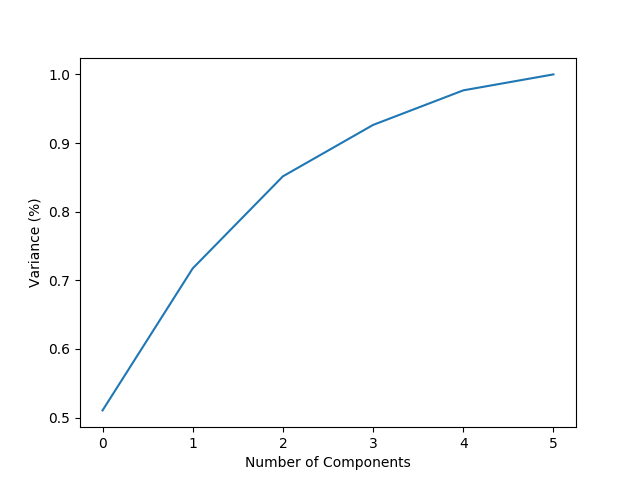
\includegraphics[width=0.5\textwidth]{imagenes/Cap3/pca}
  \caption{Gr\'{a}fico de la varianza vs el n\'{u}mero de componentes.}
  \label{fig:varianza-pca}
  \end{center}
\end{figure}

El Gr\'{a}fico \ref{fig:varianza-pca} indica que seleccionando 4 componentes se puede preservar alrededor del 95\% de la varianza total de los datos y que seleccionando 3 componentes se conserva alrededor del 80\% de la varianza de los datos, usar cualquiera de esas cantidades de componentes tiene sentido, ya que no se usar\'{a} el 100\% de la varianza, porque denota todos los componentes y s\'{o}lo se desea usar los principales.


\vspace{5mm} %5mm vertical space

\section{Resumen del cap\'{i}tulo}

En este cap\'{i}tulo se ha descrito la forma en la que se realiz\'{o} la captura del conjunto de datos de conducci\'{o}n y la preparaci\'{o}n del conjunto de datos, mediante distintas t\'{e}cnicas como la selecci\'{o}n, limpieza, reducci\'{o}n y transformaci\'{o}n de datos; con el fin de que estos valores sean una mejor entrada para el algoritmo de aprendizaje autom\'{a}tico que se aplicar\'{a} en el siguiente cap\'{i}tulo.
\chapter{\uppercase{GENERATION OF THE ANOMALY DETECTION MECHANISM}}
\label{Capitulo 5}

This chapter describes the process that was followed to generate the conduction anomaly detection mechanism. As reviewed in Chapter 3, in this document, an outlier detector with a semi-supervised approach is proposed; however, before delving into the proposed method, a description of the development environment with which the experiment was used should be carried out, in addition to reviewing dataset available in this study.
%Este cap\'{i}tulo describe el proceso que se sigui\'{o} para la generaci\'{o}n del mecanismo de detecci\'{o}n de anomal\'{i}as de conducci\'{o}n. Seg\'{u}n lo repasado en el cap\'{i}tulo 3, en el presente trabajo, se propone un detector de valores at\'{i}picos con un enfoque semi-supervisado; sin embargo, antes de profundizar en el m\'{e}todo propuesto se debe realizar una descripci\'{o}n del entorno de desarrollo con el se que desarroll\'{o} el experimento, adem\'{a}s de realizar un repaso del conjunto de datos con el que se cuenta en este estudio.

\section{Development environment}

The experiment of this study was developed on a laptop with following characteristics:
%El experimento de este estudio fue desarrollado en una computador port\'{a}til con las siguientes caracter\'{i}sticas:

\begin{itemize}
\item Intel Core i5-5200U 2.2GHz processor (c / TB 2.7 GHz).
\item 8 GB of RAM.
\item ArchLinux Operating System version 4.15.15-1-ARCH (64 bits).
%\item Procesador Intel Core i5-5200U 2.2GHz (c/TB 2.7 GHz).
%\item 8 GB de memoria RAM.
%\item Sistema Operativo ArchLinux version 4.15.15-1-ARCH (64 bits). 
\end{itemize}

It is important to clarify that methods' types used in this study are usually much more efficient in computers that have a graphics processing unit (GPU), since this unit allows parallel processing. The code developed in this work was written in \textsc{PYTHON}, an interpreted programming language that emphasizes code simplicity and readability, as well as being powered with support of powerful scientific libraries such as \textsc{NUMPY}, \textsc{SCIPY}, \textsc{OPENCV}, \textsc{KERAS}, \textsc{MATPLOTLIB}, \textsc{SEABORN}, etc. as for the experiments' development and the generation of detection mechanism, Jupyter Notebook was used, which is a local Python-based web application that allows you to view and execute documents that contain source code and equations. The versions of tools used are detailed below.
%Es importante aclarar que el tipo de m\'{e}todos utilizado en este estudio suelen ser mucho m\'{a}s eficientes en computadores que cuenten con una unidad de procesamiento gr\'{a}fico (GPU), dado que esta unidad permite el procesamiento en paralelo. El c\'{o}digo desarrollado en este trabajo fue escrito en \textsc{Python}, un lenguaje de programaci\'{o}n interpretado que se enfatiza en la simplicidad y legibilidad de c\'{o}digo, adem\'{a}s de que se potencia con el apoyo de poderosas librer\'{i}as cient\'{i}ficas tales como \textsc{NumPy}, \textsc{SciPy}, \textsc{OpenCV}, \textsc{Keras}, \textsc{Matplotlib}, \textsc{Seaborn}, etc. En cuanto al desarrollo de experimentos y la generaci\'{o}n del mecanismo de detecci\'{o}n esta desarrollado en Jupyter Notebook que es una aplicaci\'{o}n web local basado en Python que permite visualizar y ejecutar documentos que contienen c\'{o}digo fuente y ecuaciones. Las versiones de las herramientas utilizadas son detalladas a continuaci\'{o}n:

\begin{itemize}
\item \textbf{Python:} 3.6.5

\item \textbf{Jupyter:} 4.3

\item \textbf{Keras:} 2.2.2

\item \textbf{Tensorflow:} 1.11.0

\item \textbf{Scikit-learn:} 0.19.1

\item \textbf{Matplotlib:} 2.0.2
\end{itemize}

\section{Normal and anomalous dataset}

En el Cap\'{i}tulo 4 se describi\'{o} el proceso de captura y preparaci\'{o}n del conjunto de datos, as\'{i} como tambi\'{e}n su divisi\'{o}n en conjunto de entrenamiento/desarrollo/prueba; sin embargo cabe aclarar que aquel cap\'{i}tulo s\'{o}lo se enfoc\'{o} en el \textbf{conjunto de datos normales}.%, con los cuales se entrenar\'{a} el modelo ajustado al comportamiento normal.%; por lo que es el conjunto que se usa para entrenar el modelo que se ajusta al comportamiento normal de manejo.

\vspace{5mm} %5mm vertical space

A pesar de que se cuenta con una gran cantidad de datos normales, es necesario recolectar muestras que corresponden a anomal\'{i}as, con el objetivo de poder validar el m\'{e}todo que se propone en este proyecto. Por lo tanto, se realiz\'{o} la captura de un conjunto de \textbf{datos an\'{o}malos}, el cual est\'{a} conformado seg\'{u}n el Cuadro \ref{table:conjunto_anomalias}.

\begin{table}[H]
\centering
\begin{tabular}{|l|l|l|}
\hline
\textbf{Tipo de anomal\'{i}a} & \textbf{No. anomal\'{i}as} & \textbf{No. datos} \\ \hline
Giros en Zig Zag & 5 & 105  \\ \hline
Giros a la derecha e izquierda a alta velocidad & 7 & 35  \\ \hline
Frenos en seco & 6 & 24 \\ \hline
\end{tabular}
\caption{Tabla del conjunto de anomal\'{i}as (Elaboraci\'{o}n propia).}
\label{table:conjunto_anomalias}
\end{table}

\vspace{5mm} %5mm vertical space

Como se mencion\'{o} en el p\'{a}rrafo anterior el conjunto de anomal\'{i}as fue capturado para validar el m\'{e}todo propuesto, por lo tanto este conjunto se etiquet\'{o} como positivo (con la etiqueta 1) y el conjunto de datos normales como negativo (con la etiqueta 0).

\subsection{Generaci\'{o}n de series temporales}

Para la generaci\'{o}n del modelo detector de anomal\'{i}as se decidi\'{o} ir m\'{a}s all\'{a} de una simple detecci\'{o}n de anomal\'{i}as puntuales y as\'{i} poder detectar anomal\'{i}as contextuales o colectivas; debido a ello se requiere el uso de datos en series de tiempo.

\vspace{5mm} %5mm vertical space

Los datos capturados por el dispositivo m\'{o}vil, son dependientes del tiempo cronom\'{e}trico en el que fueron capturados (un dato por segundo); por lo cual el primer paso a realizar es la generaci\'{o}n de peque\~{n}as fracciones de series temporales. En la Figura \ref{fig:series-de-tiempo} se presenta los resultados de diferentes tama\~{n}os de series de tiempo, observando estos resultados en primera instancia se descarta la serie de tiempo que cuenta con dos pasos; debido a que no es lo suficientemente descriptiva. En cuanto a las series de tiempo restantes no es posible definir a\'{u}n cual es la cantidad correcta de pasos, por lo cual, ser\'{a} un par\'{a}metro a optimizar en los diferentes experimentos que se realizar\'{a} en las siguientes secciones. Cabe recalcar que el dominio de \'{e}sta variable est\'{a} entre 3 y 5 pasos.

\begin{figure}[H]
        \centering
        
\fbox{\begin{varwidth}{\textwidth}

        \centering
        \begin{subfigure}[h]{0.45\textwidth} 
            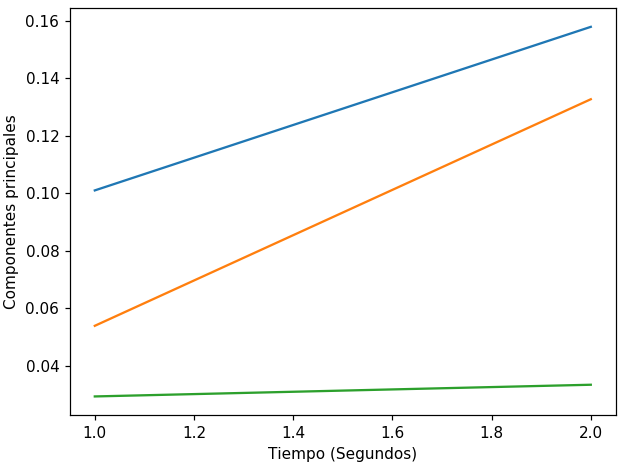
\includegraphics[width=\textwidth]{imagenes/Cap4/pca3-2}
            \caption{Serie de tiempo de 2 pasos.}
            \label{fig:pasos2}
        \end{subfigure}       
        \begin{subfigure}[h]{0.45\textwidth} 
            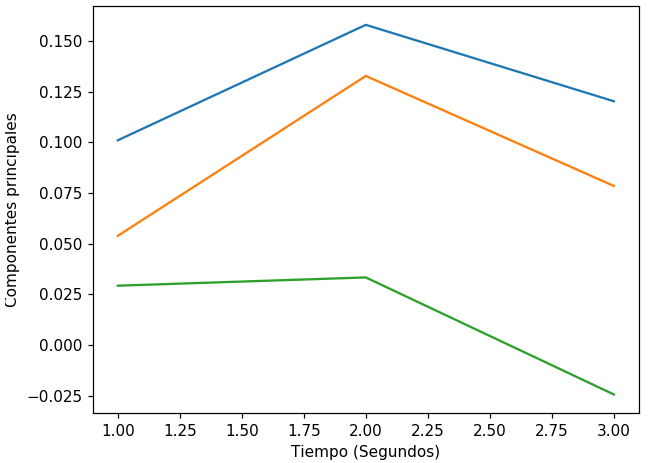
\includegraphics[width=\textwidth]{imagenes/Cap4/pca3-3}
            \caption{Serie de tiempo de 3 pasos.}
            \label{fig:pasos3}
        \end{subfigure}
        
        \begin{subfigure}[h]{0.45\textwidth} 
            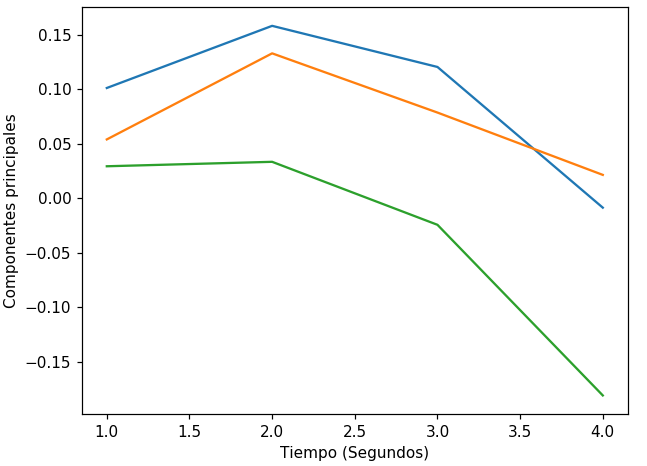
\includegraphics[width=\textwidth]{imagenes/Cap4/pca3-4}
            \caption{Serie de tiempo de 4 pasos.}
            \label{fig:pasos4}
        \end{subfigure}       
        \begin{subfigure}[h]{0.45\textwidth} 
            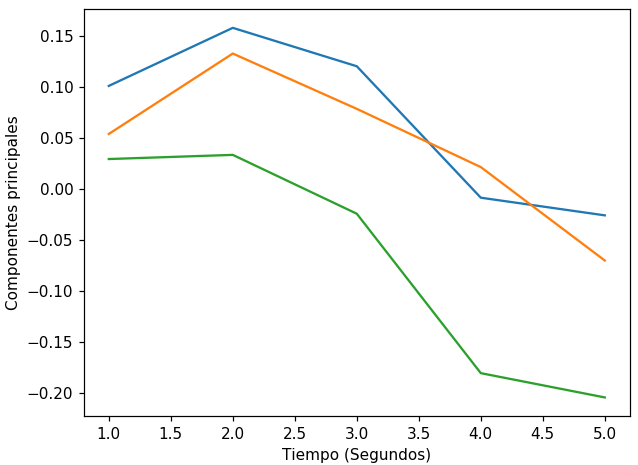
\includegraphics[width=\textwidth]{imagenes/Cap4/pca3-5}
            \caption{Serie de tiempo de 5 pasos.}
            \label{fig:pasos5}
        \end{subfigure}
        \end{varwidth}}
        \caption{Gr\'{a}fica resultante de diferentes tama\~{n}os de series de tiempo (Elaboraci\'{o}n propia).}
        
		\label{fig:series-de-tiempo}
    \end{figure}
\section{Modelo de detecci\'{o}n de anomal\'{i}as}

La presente investigaci\'{o}n propone un m\'{e}todo de detecci\'{o}n de anomal\'{i}as de conducci\'{o}n siguiendo un enfoque semi-supervisado, el cual consta de dos componentes: un \textbf{modelo del comportamiento normal} y un \textbf{m\'{e}todo para la detecci\'{o}n de valores at\'{i}picos}.

\vspace{5mm} %5mm vertical space

Por lo tanto, se realiz\'{o} la comparaci\'{o}n entre 3 diferentes m\'{e}todos de detecci\'{o}n, y seg\'{u}n el rendimiento de cada uno se elegi\'{o} la mejor opci\'{o}n. En el Cuadro \ref{table:metodos_comparados} se presenta los tres diferentes m\'{e}todos que fueron comparados; donde se puede observar que en todos los casos se usa un autoencoder como modelo del comportamiento normal, de esta manera, las siguientes secci\'{o}nes describir\'{a}n la elecci\'{o}n del autoencoder y la elecci\'{o}n de uno de los tres diferentes m\'{e}todos de detecci\'{o}n de anomal\'{i}as propuestos.

\begin{table}[H]
\centering
\begin{tabular}{|l|p{100mm}|}
\hline
\textbf{M\'{e}todo} & \textbf{Descripci\'{o}n} \\ \hline
AE\_T & M\'{e}todo de detecci\'{o}n basado en autoencoders y umbralizaci\'{o}n (Thresholding). \\ \hline
AE\_IF & M\'{e}todo de detecci\'{o}n basado en autoencoders y aplicaci\'{o}n de Isolation Forest.  \\ \hline
AE\_OC-SVM & M\'{e}todo de detecci\'{o}n basado en autoencoders y aplicaci\'{o}n de One-Class SVM. \\ \hline
\end{tabular}
\caption{Tabla de los m\'{e}todos comparados (Elaboraci\'{o}n propia).}
\label{table:metodos_comparados}
\end{table}

\subsection{Modelo del comportamiento normal}

Esta etapa es una de las partes m\'{a}s importantes de \'{e}ste trabajo, debido a que el rendimiendo del modelo de detecci\'{o}n de anomal\'{i}as depende en gran parte de la precisi\'{o}n de esta etapa.

\subsubsection{Arquitectura del modelo}

Como se mencion\'{o} en la anterior secci\'{o}n en esta etapa se utilizar\'{a} un autoencoder como modelo ajustado al comportamiento normal de conducci\'{o}n. Por lo cual el autoencoder se entren\'{o} con el conjunto de datos normales, de manera que el modelo aprenda a generar s\'{o}lo las clases que se consideran normales y, con suerte, tendr\'{a} problemas para reconstruir anomal\'{i}as, debido a que estas muestras no fueron presentadas durante el entrenamiento.

\vspace{5mm} %5mm vertical space

Para ello se prob\'{o} con diferentes arquitecturas, primero la forma m\'{a}s simple que s\'{o}lo se basa el uso de capas densas (completamente conectadas), luego se hizo pruebas con redes convolucionales y por \'{u}ltimo con redes recurrentes haciendo uso espec\'{i}fico de capas LSTM. Por cada tipo de red se hizo la prueba con 3 diferentes tipos de entrada, es decir, se prob\'{o} una diferente cantidad de pasos (entre 3 y  5) en las series temporales. Por lo tanto se realizaron 9 diferentes experimentos, de los cuales por cada tipo de red sobresali\'{o} una (usando la precisi\'{o}n de las redes como tipo de evaluaci\'{o}n para desarrollar las comparaciones).

\vspace{5mm} %5mm vertical space

En el Cuadro \ref{table:dense33} se presenta la red que obtuvo el mejor resultado de todas las Redes Densas que se probaron, esta red corresponde a la red que fue alimentada con secuencias de 3 pasos. Esta red cuenta con una capa de entrada (Input), una capa de aplanamiento (Flatten) esto debido a que la capa de entrada recibe una entrada bidimensional, un conjunto de capas densas (Dense) que van comprimiendo la informaci\'{o}n de los datos de entrada para posteriormente reconstruirlos, y por \'{u}ltimo la capa de salida es solo una capa para modificar la forma de la salida (Reshape); otro punto importante a resaltar es que las capas internas usan $elu$ como funci\'{o}n de activaci\'{o}n y la \'{u}ltima capa densa utilizan una funci\'{o}n de activaci\'{o}n tangencial ($tanh$), esto se debe a que el conjunto de datos, posterior a la obtenci\'{o}n de componentes principales, se encuentra en el rango $(1, -1)$.

\begin{table}[H]
\centering
\begin{center}
\begin{tabular}{ll|l|r|l|r|}
\cline{3-6}
                                                    &                             & \multicolumn{4}{c|}{\textbf{Arquitectura Densa}}                                                                                                           \\ \cline{3-6} 
                                                    &                             & \multicolumn{4}{c|}{\textbf{NN\_33}}                                                                                                                                   \\ \cline{3-6} 
                                                    &                             & \multicolumn{1}{c|}{\textbf{Tipo}} & \multicolumn{1}{c|}{\textbf{Salida}} & \multicolumn{1}{c|}{\textbf{Activaci\'{o}n}} & \multicolumn{1}{l|}{\textbf{\# Par\'{a}metros}} \\ \hline
\multicolumn{1}{|l|}{\multirow{7}{*}{\textbf{PCA}}} & \multirow{7}{*}{\textbf{3}} & Input                              & (3,3)                                &                                          & 0                                           \\ \cline{3-6} 
\multicolumn{1}{|l|}{}                              &                             & Flatten                            & 9                                    &                                          & 0                                           \\ \cline{3-6} 
\multicolumn{1}{|l|}{}                              &                             & Dense                              & 8                                   & elu                                     & 80                                          \\ \cline{3-6} 
\multicolumn{1}{|l|}{}                              &                             & Dense                              & 5                                   & elu                                     & 45                                          \\ \cline{3-6} 
\multicolumn{1}{|l|}{}                              &                             & Dense                              & 8                                    & elu                                     & 88                                          \\ \cline{3-6} 
\multicolumn{1}{|l|}{}                              &                             & Dense                              & 9                                    & tanh                                     & 81                                          \\ \cline{3-6} 
\multicolumn{1}{|l|}{}                              &                             & Reshape                            & (3,3)                                &                                          & 0                                           \\ \hline
\end{tabular}
\end{center}
\caption{Arquitectura densa para una secuencia de 3 pasos y 3 componentes principales (Elaboraci\'{o}n propia).}
\label{table:dense33}
\end{table}

% ejemplos de cuadros de aruqitecturas de redes https://webthesis.biblio.polito.it/10360/1/tesi.pdf

% metricas de evaluacion http://www.diva-portal.org/smash/get/diva2:1225367/FULLTEXT01.pdf  , https://escholarship.org/content/qt1f03f6hb/qt1f03f6hb.pdf  ,   http://www.nada.kth.se/~ann/exjobb/maxim_wolpher.pdf

% Ejemplo cuadros resultados    https://arxiv.org/pdf/1809.00957.pdf 

Por otra parte el Cuadro \ref{table:cnn33} se presenta la red que obtiene la mejor precisi\'{o}n de todas las Redes Convolucionales que fueron probadas, esta red al igual que la anterior corresponde a la red que fue alimentada con secuencias de 3 pasos. Su arquitectura consta de una capa de entrada (Input), una combinaci\'{o}n de capas de convoluci\'{o}n de una dimensi\'{o}n (Conv1D) y agrupaci\'{o}n (MaxPooling1D) hasta comprimir los datos a una dimensi\'{o}n de (2,4), luego un conjunto de capas convolucionales y de muestra ascendente (Upsampling1D) para decodificar la informaci\'{o}n compresa. Cabe recalcar que esta red tambi\'{e}n usa la funci\'{o}n de activaci\'{o}n tangencial en su \'{u}ltima capa por las razones que se explicaron en el p\'{a}rrafo anterior.

\begin{table}[H]
\centering
\begin{center}
\begin{tabular}{ll|l|r|l|r|}
\cline{3-6}
                                                    &                             & \multicolumn{4}{c|}{\textbf{Arquitectura Convolucional}}                                                                                                           \\ \cline{3-6} 
                                                    &                             & \multicolumn{4}{c|}{\textbf{CNN\_33}}                                                                                                                                  \\ \cline{3-6} 
                                                    &                             & \multicolumn{1}{c|}{\textbf{Tipo}} & \multicolumn{1}{c|}{\textbf{Salida}} & \multicolumn{1}{c|}{\textbf{Activaci\'{o}n}} & \multicolumn{1}{l|}{\textbf{\# Par\'{a}metros}} \\ \hline
\multicolumn{1}{|l|}{\multirow{8}{*}{\textbf{PCA}}} & \multirow{8}{*}{\textbf{3}} & Input                              & (3,3)                                &                                          & 0                                           \\ \cline{3-6} 
\multicolumn{1}{|l|}{}                              &                             & Conv1D                             & (3,2)                                & elu                                     & 20                                          \\ \cline{3-6} 
\multicolumn{1}{|l|}{}                              &                             & MaxPooling1D                       & (2,2)                                &                                          & 0                                           \\ \cline{3-6} 
\multicolumn{1}{|l|}{}                              &                             & Conv1D                             & (2,4)                                & elu                                     & 28                                          \\ \cline{3-6} 
\multicolumn{1}{|l|}{}                              &                             & MaxPooling1D                       & (1,4)                                &                                          & 0                                           \\ \cline{3-6} 
\multicolumn{1}{|l|}{}                              &                             & Conv1D                             & (1,6)                                & elu                                     & 54                                          \\ \cline{3-6} 
\multicolumn{1}{|l|}{}                              &                             & UpSampling1D                       & (3,6)                                &                                          & 0                                           \\ \cline{3-6} 
\multicolumn{1}{|l|}{}                              &                             & Conv1D                             & \multicolumn{1}{l|}{(3,3)}           & tanh                                     & 57                                          \\ \hline
\end{tabular}
\end{center}
\caption{Arquitectura convolucional para una secuencia de 3 pasos y 3 componentes principales (Elaboraci\'{o}n propia).}
\label{table:cnn33}
\end{table}

% lstm autoencode

En el Cuadro \ref{table:rnn33} se muestra la red que obtuvo la mejor precisi\'{o}n de todas las Redes Recurrentes probadas, como en los anteriores casos \'{e}sta red es alimentada con secuencias de 3 pasos. Dicha red cuenta con una capa de entrada (Input), dos capas LSTM una que retorna sus secuencias y una que no, luego viene una capa de redimensionado, posteriormente dos capas LSTM, y finalmente un contenedor  (TimeDistributed) de una capa densa.

\begin{table}[H]
\centering
\begin{center}
\begin{tabular}{ll|l|r|l|r|}
\cline{3-6}
                                                    &                             & \multicolumn{4}{c|}{\textbf{Arquitectura Recurrente}}                                                                                                           \\ \cline{3-6} 
                                                    &                             & \multicolumn{4}{c|}{\textbf{RNN\_33}}                                                                                                                                  \\ \cline{3-6} 
                                                    &                             & \multicolumn{1}{c|}{\textbf{Tipo}} & \multicolumn{1}{c|}{\textbf{Salida}} & \multicolumn{1}{c|}{\textbf{Activaci\'{o}n}} & \multicolumn{1}{l|}{\textbf{\# Par\'{a}metros}} \\ \hline
\multicolumn{1}{|l|}{\multirow{7}{*}{\textbf{PCA}}} & \multirow{7}{*}{\textbf{3}} & Input                              & (3,3)                                &                                          & 0                                           \\ \cline{3-6} 
\multicolumn{1}{|l|}{}                             &                             & LSTM                               & (3,9)                                & elu                                     & 468                                         \\ \cline{3-6} 
\multicolumn{1}{|l|}{}                              &                             & LSTM                               & 6                                    & elu                                     & 384                                         \\ \cline{3-6} 
\multicolumn{1}{|l|}{}                              &                             & Reshape                            & (3,2)                                &                                          & 0                                           \\ \cline{3-6} 
\multicolumn{1}{|l|}{}                              &                             & LSTM                               & (3,3)                                & elu                                     & 72                                          \\ \cline{3-6} 
\multicolumn{1}{|l|}{}                              &                             & LSTM                               & (3,9)                                & elu                                     & 468                                         \\ \cline{3-6} 
\multicolumn{1}{|l|}{}                              &                             & TimeDistributed(Dense)             & (3,3)                                & tanh                                     & 30                                          \\ \hline
\end{tabular}
\end{center}
\caption{Arquitectura recurrente para una secuencia de 3 pasos y 3 componentes principales (Elaboraci\'{o}n propia).}
\label{table:rnn33}
\end{table}

Es importante recalcar que las capas de redimensi\'{o}n, agrupaci\'{o}n, muestra ascendente y contenedores s\'{o}lo fueron usadas para controlar la correcta compresi\'{o}n y descompresi\'{o}n de los autoencoders, es por ello que no se detalla a profundidad su funcionamiento.

\vspace{5mm} %5mm vertical space

\textbf{Evaluaci\'{o}n de autoencoders}

\vspace{5mm} %5mm vertical space

Anteriormente se present\'{o} los mejores representantes por tipo de red; ahora se proceder\'{a} a la evaluaci\'{o}n y comparaci\'{o}n de estos 3 tipos de autoencoders, con el objetivo de elegir la arquitectura que se ajusta mejor al comportamiento normal de conducci\'{o}n.

\vspace{5mm} %5mm vertical space

En el Cap\'{i}tulo 3 se present\'{o} los diversos tipos de evaluaci\'{o}n que existen, en esta etapa el tipo de evaluaci\'{o}n m\'{a}s apropiado es la \textbf{precisi\'{o}n} del modelo, debido a que se tiene un gran conjunto de datos balanceado (debido a que s\'{o}lo se cuenta con comportamientos normales de conducci\'{o}n que correspoden a una sola clase, la "Normal"). Los resultados de la evaluaci\'{o}n de los tres tipos de redes son mostrados en el Cuadro \ref{table:evaluacion_redes}; dicho cuadro presenta la precisi\'{o}n, p\'{e}rdida logar\'{i}tmica y tiempo de ejecuci\'{o}n de cada autoencoder seg\'{u}n el conjunto de prueba; observando estos resultados se puede apreciar que las dos mejores redes son la red densa \textbf{NN\_33} y la red recurrente \textbf{RNN\_33} con precisiones de 90\% aproximadamente, adem\'{a}s de presentar un valor de p\'{e}rdida relativamente bajo en comparaci\'{o}n a la red \textbf{CNN\_33}.

\begin{table}[H]
\centering
\begin{center}
\begin{tabular}{|l|r|r|r|}
\hline
\textbf{Red} & \multicolumn{1}{l|}{\textbf{Precisi\'{o}n}} & \multicolumn{1}{l|}{\textbf{Loss}} & \multicolumn{1}{l|}{\textbf{Tiempo ejecuci\'{o}n}} \\ \hline
NN\_33              & 0.9000740711953905  & 0.003956934471097257  & 26us/step  \\ \hline
CNN\_33             & 0.8437777761353387  & 0.006740666443275081  & 31us/step  \\ \hline
RNN\_33             & 0.8899259290695191  & 0.003611267575787173  & 101us/step \\ \hline
\end{tabular}
\end{center}
\caption{Evaluaci\'{o}n de las redes NN\_33, CNN\_33 y RNN\_33  (Elaboraci\'{o}n propia).}
\label{table:evaluacion_redes}
\end{table}

Por otra parte la diferencia m\'{a}s grande entre las dos mejores redes (\textbf{NN\_33} y \textbf{RNN\_33}) es el tiempo de ejecuci\'{o}n ya que de la primera es de tan solo 26 segundos/paso y de la segunda es de 101 segundos/paso, debido a estas similitudes entre ambas redes es necesario verificar visualmente los resultados de reconstrucci\'{o}n de cada tipo de red, de tal manera que se pueda elegir la red m\'{a}s adecuada para este problema. 

\vspace{5mm} %5mm vertical space

En la Figura \ref{fig:res_autoencoders} se muestra los resultados de los autoencoders de siete secuencias tomadas aleatoriamente del conjunto de prueba, en la parte superior de cada figura se encuentra la secuencia de entrada y en la inferior la reconstrucci\'{o}n del modelo, como ya se pod\'{i}a esperar la red \textbf{CNN\_33} presenta los peores resultados, lo cual hace que dicha red sea descartada; en cuanto a las dos redes restantes, la red \textbf{NN\_33} presenta reconstrucciones muy similares a las secuencias de entrada, con algunos peque\~{n}os errores; por otra parte \textbf{RNN\_33} presenta errores un poco m\'{a}s notorios que los obtenidos por  \textbf{NN\_33}. Por lo tanto se lleg\'{o} a la conclusi\'{o}n de que la red \textbf{NN\_33} se ajusta mejor al comportamiento normal de conducci\'{o}n, adem\'{a}s de tener la gran ventaja de tener un tiempo de ejecuci\'{o}n mucho menor que el de \textbf{RNN\_33}, lo cual es realmente importante para los sistemas en tiempo real as\'{i} como tambi\'{e}n de aquellos que cuentan con recursos de ejecuci\'{o}n limitados, como es el caso del presente trabajo.

\begin{figure}
        \centering
        
\fbox{\begin{varwidth}{\textwidth}

        \centering
        \begin{subfigure}[h]{0.99\textwidth} 
            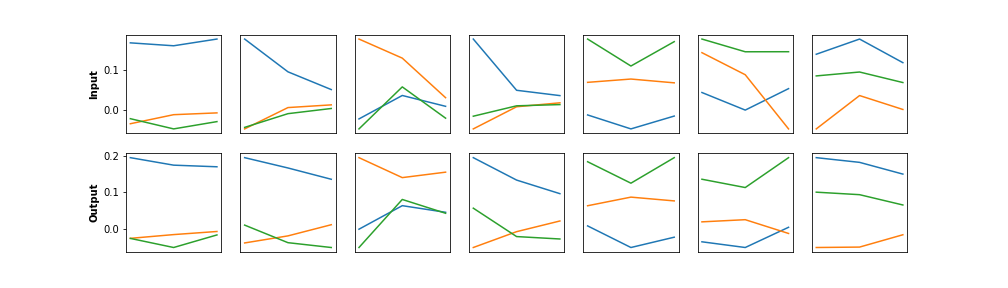
\includegraphics[width=\textwidth]{imagenes/Cap5/resultado_nn}
            \caption{Resultados de la red \textbf{NN\_33}}
            \label{fig:res_nn}
        \end{subfigure}       
        \begin{subfigure}[h]{0.99\textwidth} 
            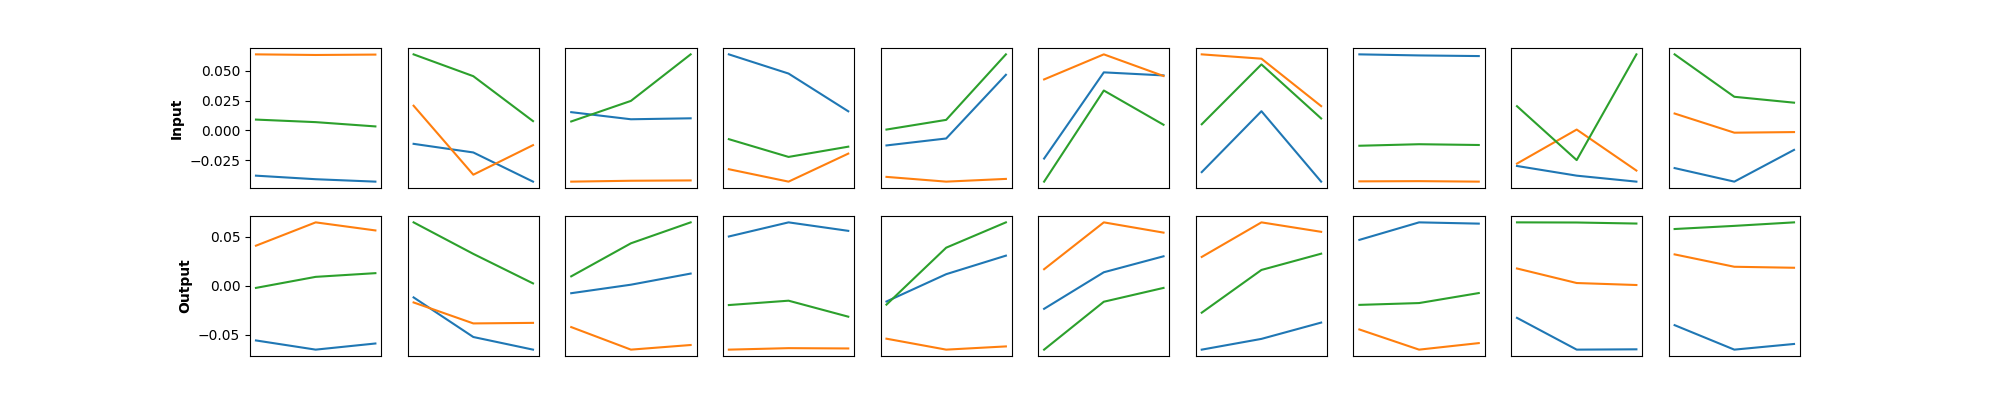
\includegraphics[width=\textwidth]{imagenes/Cap5/resultado_cnn}
            \caption{Resultados de la red \textbf{CNN\_33}}
            \label{fig:res_cnn}
        \end{subfigure}
        
        \begin{subfigure}[h]{0.99\textwidth} 
            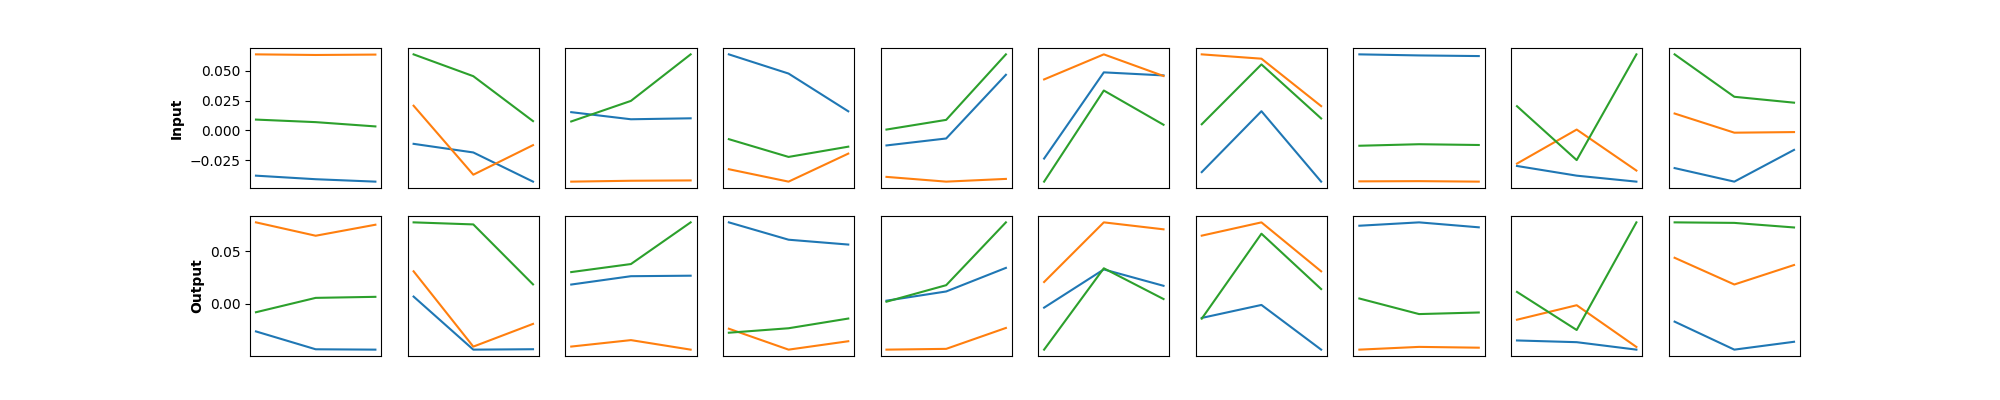
\includegraphics[width=\textwidth]{imagenes/Cap5/resultado_rnn}
            \caption{Resultados de la red \textbf{RNN\_33}}
            \label{fig:res_rnn}
        \end{subfigure}     
        \end{varwidth}}
        \caption{Resultados (Elaboraci\'{o}n propia).}
        
		\label{fig:res_autoencoders}
    \end{figure}


\vspace{5mm} %5mm vertical space

Una vez definido como est\'{a} constituido el modelo del comportamiento normal se puede proceder con la elecci\'{o}n del m\'{e}todo de detecci\'{o}n de valores at\'{i}picos.

\subsection{M\'{e}todo de detecci\'{o}n de anomal\'{i}as}

Al inicio de esta secci\'{o}n se defini\'{o} tres diferentes enfoques para la detecci\'{o}n de anomal\'{i}as: la umbralizaci\'{o}n, la aplicaci\'{o}n de bosques de aislamiento y finalmente la aplicaci\'{o}n de SVM para una clase.

\subsubsection{Umbralizaci\'{o}n}

Esta t\'{e}cnica se basa en la definici\'{o}n de un umbral para determinar si el error de reconstrucci\'{o}n  que obtiene el autoencoder (modelo del comportamiento normal) es lo suficientemente alto como para considerarse un valor at\'{i}pico. Por lo tanto primero se debe definir la ecuaci\'{o}n del error de reconstrucci\'{o}n para el modelo. En el presente trabajo el error de reconstrucci\'{o}n se define seg\'{u}n la ecuaci\'{o}n \ref{eqn:error_rec}, donde $x_{i}$ representa el valor real (entrada del autoencoder) y $\hat{x_{i}}$ representa el valor obtenido por el autoencoder (salida del autoencoder).

\begin{equation}
\textup{Error de reconstrucci\'{o}n} = S_{z} = |x_{i} - \hat{x_{i}}|^{2} 
\label{eqn:error_rec}
\end{equation}

En la Figura \ref{fig:codos} se muestra la curva de los errores de reconstrucci\'{o}n obtenidos con el modelo del compotamiento normal para el conjunto de muestras normales.

\begin{figure}[H]
        \centering
            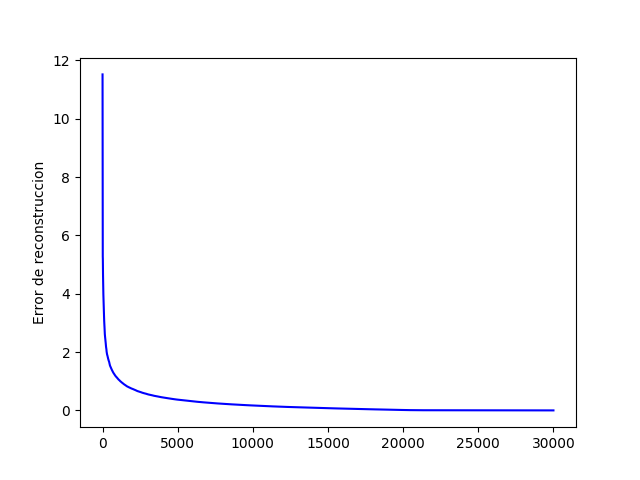
\includegraphics[width=0.75\textwidth, frame]{imagenes/Cap5/codos}
        \caption{Curva de los valores de reconstrucci\'{o}n obtenidos con el modelo del comportamiento normal (Elaboraci\'{o}n propia).}
		\label{fig:codos}
    \end{figure}

Una vez definido la ecuaci\'{o}n de reconstrucci\'{o}n, se debe definir un umbral capaz de poder detectar la mayor cantidad de anomal\'{i}as posibles. Esta tarea puede tornarse simple en un entorno de aprendizaje supervisado, sin embargo automatizar esta tarea en un contexto de aprendizaje no supervisado es un desaf\'{i}o que puede ser dif\'{i}cil de sobrellevar. En el presente trabajo se us\'{o} una t\'{e}cnica basada en encontrar un \textit{Punto de codo} de una curva, que en este caso la curva est\'{a} construida en base a los errores de reconstrucci\'{o}n del autoencoder.

\vspace{5mm} %5mm vertical space

% https://github.com/arvkevi/kneed
Existen diferentes formas de hallar el punto de codo, sin embargo en este trabajo se utiliz\'{o} una herramienta de Python, que automatiza esta tarea, llamada Kneedle. Esta herramienta devuelve el punto de inflexi\'{o}n de la funci\'{o}n de la curva obtenida por el conjunto de valores proporcionado \textit{x} y \textit{y}, cabe recalcar que el punto de codo es el punto de m\'{a}xima curvatura, por otra parte esta herramienta cuenta con un par\'{a}metro de sensibilidad (S), este par\'{a}metro permite ajustar qu\'{e} tan agresivo se desea ser al detectar codos, los valores m\'{a}s peque\~{n}os para S detectan los codos m\'{a}s r\'{a}pido, mientras que los m\'{a}s grandes son m\'{a}s conservadores, es decir, S es una medida de cu\'{a}ntos puntos ''planos'' se espera ver en la curva de datos sin modificar antes de declarar un codo.

\vspace{5mm} %5mm vertical space

De esta manera en el presente proyecto se realiz\'{o} experimentos con diferentes valores de sensibilidad para encontrar el codo m\'{a}s adecuado para el conjunto de datos con el que se trabajo. En la Figura \ref{fig:zoom_codos}, se muestra los diferentes codos hallados para los valores de sensibilidad proporcionados (valores entre 0 y 2).

\begin{figure}[H]
        \centering
            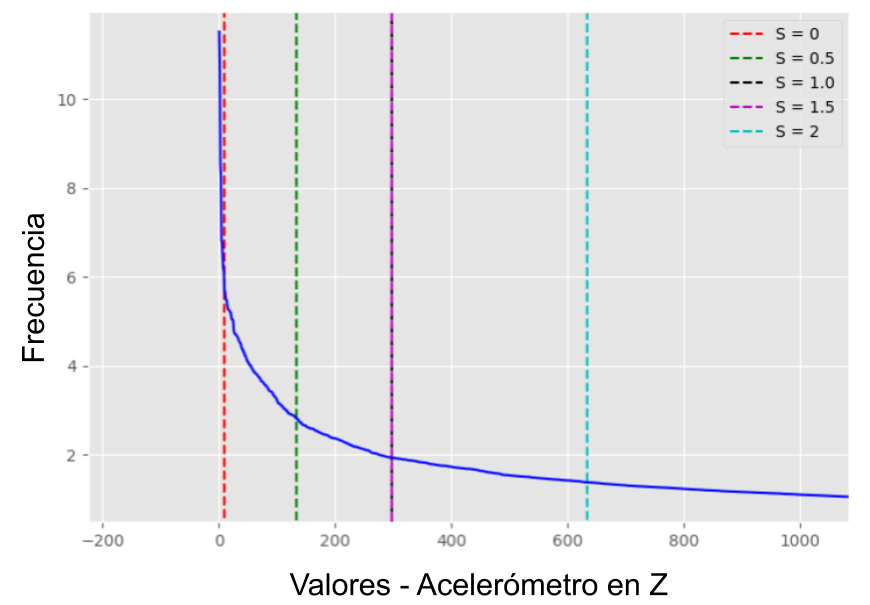
\includegraphics[width=0.75\textwidth, frame]{imagenes/Cap5/zoom_codos}
        \caption{Resultados de la obtenci\'{o}n de codos con diferentes valores de Sensibilidad, para los valores de reconstrucci\'{o}n obtenidos con el modelo del comportamiento normal (Elaboraci\'{o}n propia).}
		\label{fig:zoom_codos}
\end{figure}

Una vez obtenidos los codos se realiz\'{o} la evaluaci\'{o}n de cada uno de ellos, en el Cuadro \ref{table:evaluacion_codos} se presentan el umbral, los valores de la matriz de confusi\'{o}n, la sensibilidad y especifidad para cada codo. Los valores de la matriz de confusi\'{o}n son el resultado de aplicar el umbral de cada codo a los errores de reconstrucci\'{o}n obtenidos del conjunto de datos total (conjunto de datos normal y anormal equivalente a 44204 datos).

\begin{table}[H]
\centering
\begin{center}
\begin{tabular}{|l|r|r|r|r|r|r|r|}
\hline
\textbf{S} & \multicolumn{1}{l|}{\textbf{Umbral}} & \multicolumn{1}{l|}{\textbf{VP}} & \multicolumn{1}{l|}{\textbf{VN}}& \multicolumn{1}{l|}{\textbf{FN}}& \multicolumn{1}{l|}{\textbf{FP}} & \multicolumn{1}{l|}{\textbf{Sensibilidad}} & \multicolumn{1}{l|}{\textbf{Especificidad}} \\ \hline
0.0 & 5.665 & \cellcolor[HTML]{AADD99} 92 & \cellcolor[HTML]{AADD99} 43993 & \cellcolor[HTML]{FFCE93} 72 & \cellcolor[HTML]{FFCE93} 47 & 0.5610 & 0.9989 \\ \hline
0.5  & 2.806 & \cellcolor[HTML]{AADD99} 111 & \cellcolor[HTML]{AADD99} 43814 & \cellcolor[HTML]{FFCE93} 53 & \cellcolor[HTML]{FFCE93} 226 & 0.6768 & 0.9949 \\ \hline
1.0 &  1.920 & \cellcolor[HTML]{AADD99} 120 & \cellcolor[HTML]{AADD99} 43562 & \cellcolor[HTML]{FFCE93} 44 & \cellcolor[HTML]{FFCE93} 478 & 0.7317 & 0.9891 \\ \hline
2.0 & 1.369	 & \cellcolor[HTML]{AADD99} 128 & \cellcolor[HTML]{AADD99} 43100  & \cellcolor[HTML]{FFCE93} 36 & \cellcolor[HTML]{FFCE93} 940 & 0.7805 & 0.9787 \\ \hline
\end{tabular}
\end{center}
\caption{Evaluaci\'{o}n de la detecci\'{o}n de anomal\'{i}as para cada codo obtenido con los diferentes valores de sensibilidad (Elaboraci\'{o}n propia).}
\label{table:evaluacion_codos}
\end{table}

Seg\'{u}n los resultados que se muestran en el Cuadro \ref{table:evaluacion_codos} se puede decir que mientras m\'{a}s peque\~{n}o es el umbral la sensibilidad (proporci\'{o}n de anomal\'{i}as detectadas correctamente como anomal\'{i}as) incrementa, sin embargo, a su vez reduce la especifidad (proporci\'{o}n de valores normales correctamente detectados como valores normales). Por lo tanto se debe hallar un punto intermedio, donde se pueda detectar la mayor cantidad de anomal\'{i}as posibles y reducir en lo posible la cantidad de falsos positivos (datos normales que son detectados como anomal\'{i}as). De esta forma el umbral m\'{a}s adecuado para el objetivo planteado fue 2.806, ya que con este umbral se detecta 111 anomal\'{i}as de 164 y los falsos positivos son aproximadamente el doble de los valores at\'{i}picos detectados. 

\vspace{5mm} %5mm vertical space

De ello se deduce que, para detectar autom\'{a}ticamente el umbral el uso de 0.5 como par\'{a}metro S es el m\'{a}s adecuado, sin embargo si se desea incrementar el porcentaje de detecci\'{o}n de anomal\'{i}as a costa de incrementar el n\'{u}mero de falsos positivos se puede usar un valor mayor a 0.5 para S y en caso de querer la menor cantidad de falsos positivos posibles se debe usar un valor menor a 0.5.

\subsubsection{Isolation Forest}

Antes de presentar como se llevar\'{a} a cabo los experimentos con este algoritmo, es necesario ilustrar m\'{a}s detalladamente el funcionamiento del mismo. Por lo tanto la Figura \ref{fig:isolartion-forest} representa c\'{o}mo se espera que un punto de datos anómalo se aísle rápidamente con el uso de este algoritmo, mientras que un punto de datos normal necesita más particiones para poder ser aislado.

\begin{figure}[h!]
  \begin{center}	\includegraphics[width=0.75\textwidth, frame]{imagenes/Cap5/isolation-forest}
  \caption{La figura de la izquierda muestra el aislamiento de una anomalía, que requiere solo tres particiones. A la derecha, el aislamiento de un punto normal requiere seis particiones \protect\cite{Reference60}.} 
  \label{fig:isolartion-forest}
  \end{center}
\end{figure}

Una vez detallado resumidamente el funcionamiento de los bosques de aislamiento se puede proseguir con los diferentes enfoques de los experimentos que se realizar\'{a} con Isolation Forest.

\vspace{5mm} %5mm vertical space

Existen dos enfoques que pueden realizarse con esta t\'{e}cnica; el primero entrena el modelo con los valores compresos del codificador del autoencoder y el segundo se entrena con los errores de reconstrucci\'{o}n del autoencoder. A continuaci\'{o}n se presenta una gr\'{a}fica (Ver Figura \ref{fig:autoencoder}) del autoencoder (modelo del comportamiento normal) con el fin de tener un mejor entendimiento de c\'{o}mo se realizar\'{a}n los experimentos tanto para los bosques de aislamiento como para los SVM de una clase.

\begin{figure}[H]
        \centering
            \includegraphics[width=0.75\textwidth, frame]{imagenes/Cap5/autoencoder}
        \caption{Representaci\'{o}n gr\'{a}fica del modelo de comportamiento normal o autoencoder (Elaboraci\'{o}n propia).}
		\label{fig:autoencoder}
\end{figure}

\begin{itemize}
\item \textbf{\textit{Isolation forest para valores codificados: }}Esta t\'{e}cnica entrena un modelo de bosque de aislamiento con los valores codificados (mediante el codificador del autoencoder, ver Figura \ref{fig:autoencoder}) del conjunto de entrenamiento normal. Para los experimentos se utiliz\'{o} la clase IsolationForest de \textsc{scikit-learn}, esta clase tiene un par\'{a}metro llamado \textsc{contaminaci\'{o}n} el cual sirve para definir que cantidad del conjunto de datos esta contaminado, es decir, define que cantidad de los datos de entrenamiento pueden ser valores at\'{i}picos; en la presente investigaci\'{o}n se realiz\'{o} varias pruebas con diferentes valores para el par\'{a}metro contaminaci\'{o}n. En el Cuadro \ref{table:evaluacion_IF_encoded} se presenta los resultados, donde se evidencia que ninguno de los resultados es alentador, ya que la cantidad de anomal\'{i}as detectadas es muy baja para los tres casos con los que se experimento.

\begin{table}[H]
\centering
\begin{center}
\begin{tabular}{|l|r|r|r|r|r|r|r|}
\hline
\textbf{Contaminaci\'{o}n (C)} & \multicolumn{1}{l|}{\textbf{VP}} & \multicolumn{1}{l|}{\textbf{VN}}& \multicolumn{1}{l|}{\textbf{FN}}& \multicolumn{1}{l|}{\textbf{FP}} & \multicolumn{1}{l|}{\textbf{Sensibilidad}} & \multicolumn{1}{l|}{\textbf{Especificidad}} \\ \hline
0.0025 & \cellcolor[HTML]{AADD99} 3 & \cellcolor[HTML]{AADD99} 43944 & \cellcolor[HTML]{FFCE93} 161 & \cellcolor[HTML]{FFCE93} 96 & 0.0183 & 0.9978 \\ \hline
0.0050 & \cellcolor[HTML]{AADD99} 17 & \cellcolor[HTML]{AADD99} 43817 & \cellcolor[HTML]{FFCE93} 147 & \cellcolor[HTML]{FFCE93} 223 & 0.1037 & 0.9949 \\ \hline
0.0075 & \cellcolor[HTML]{AADD99} 17 & \cellcolor[HTML]{AADD99} 43738 & \cellcolor[HTML]{FFCE93} 147 & \cellcolor[HTML]{FFCE93} 302 & 0.1037 & 0.9931 \\ \hline
\end{tabular}
\end{center}
\caption{Evaluaci\'{o}n de la detecci\'{o}n de anomal\'{i}as usando Isolation forest para valores compresos (Elaboraci\'{o}n propia).}
\label{table:evaluacion_IF_encoded}
\end{table}

\item \textbf{\textit{Isolation forest para errores de reconstrucci\'{o}n: }}Para esta t\'{e}cnica se realiz\'{o} el entrenamiento del bosque de aislamiento con la diferencia de los valores de entrada con los valores obtenidos por el autoencoder (Ver Figura \ref{fig:error}), cabe aclarar que la diferencia mencionada anteriormente tambi\'{e}n ser\'{a} llamada \textit{Error de reconstrucci\'{o}n} tanto en esta como en la siguiente subsecci\'{o}n. Los resultados de esta t\'{e}cnica para diferentes valores de contaminaci\'{o}n se presentan en el Cuadro \ref{table:evaluacion_IF_errores_reconstruccion}, donde estos resultados se pueden considerar como \'{o}ptimos, debido a que oscilan entre 62 y 67\% de detecciones correctas de anomal\'{i}as, adem\'{a}s de presentar una especificidad realmente alta, del 99\% aproximadamente, lo cual quiere decir que estos modelos presentan una baja tasa de falsos positivos. 

\begin{figure}[H]
        \centering
            \includegraphics[width=0.75\textwidth, frame]{imagenes/Cap5/error}
        \caption{Representaci\'{o}n gr\'{a}fica del error de reconstrucci\'{o}n usado para el entrenamiento de los bosques de aislamiento y los SVM de una clase (Elaboraci\'{o}n propia).}
		\label{fig:error}
\end{figure}

\begin{table}[H]
\centering
\begin{center}
\begin{tabular}{|l|r|r|r|r|r|r|r|}
\hline
\textbf{Contaminaci\'{o}n (C)} & \multicolumn{1}{l|}{\textbf{VP}} & \multicolumn{1}{l|}{\textbf{VN}}& \multicolumn{1}{l|}{\textbf{FN}}& \multicolumn{1}{l|}{\textbf{FP}} & \multicolumn{1}{l|}{\textbf{Sensibilidad}} & \multicolumn{1}{l|}{\textbf{Especificidad}} \\ \hline
0.0025 & \cellcolor[HTML]{AADD99} 103 & \cellcolor[HTML]{AADD99} 43898 & \cellcolor[HTML]{FFCE93} 61 & \cellcolor[HTML]{FFCE93} 142 & 0.6280 & 0.9968 \\ \hline
0.0050 & \cellcolor[HTML]{AADD99} 108 & \cellcolor[HTML]{AADD99} 43792 & \cellcolor[HTML]{FFCE93} 56 & \cellcolor[HTML]{FFCE93} 248 & 0.6585 & 0.9944 \\ \hline
0.0075 & \cellcolor[HTML]{AADD99} 111 & \cellcolor[HTML]{AADD99} 43688 & \cellcolor[HTML]{FFCE93} 53 & \cellcolor[HTML]{FFCE93} 352 & 0.6768 & 0.9920 \\ \hline
\end{tabular}
\end{center}
\caption{Evaluaci\'{o}n de la detecci\'{o}n de anomal\'{i}as usando Isolation forest para errores de reconstrucci\'{o}n (Elaboraci\'{o}n propia).}
\label{table:evaluacion_IF_errores_reconstruccion}
\end{table}
\end{itemize}

\subsubsection{One-Class SVM}

De la misma forma que en los bosques de aislamiento, se realiz\'{o} dos diferentes tipos de experimentos con One-Class SVM, a continuaci\'{o}n se detalla cada uno de ellos.

\begin{itemize}
\item \textbf{\textit{One-Class SVM para valores codificados: }}Se debe entrenar un modelo SVM de una clase para los valores compresos obtenidos por el autoencoder; los experimentos fueron realizados usando la clase OneClassSVM de \textsc{scikit-learn}, donde se tiene diferentes par\'{a}metros que pueden ser personalizados, para la presente investigaci\'{o}n se prob\'{o} diferentes kernels, obteniendo as\'{i} los resultados que se muestran en el Cuadro \ref{table:evaluacion_SVM_encoded}, donde claramente ninguno de los resultados obtenidos podr\'{i}a ser tomado en cuenta para ser el m\'{e}todo de detecci\'{o}n de anomal\'{i}as de conducci\'{o}n ya que la sensibilidad en ninguno de los casos es superior a 50\%.

\begin{table}[H]
\centering
\begin{center}
\begin{tabular}{|l|r|r|r|r|r|r|r|}
\hline
\textbf{Kernel} & \multicolumn{1}{l|}{\textbf{VP}} & \multicolumn{1}{l|}{\textbf{VN}}& \multicolumn{1}{l|}{\textbf{FN}}& \multicolumn{1}{l|}{\textbf{FP}} & \multicolumn{1}{l|}{\textbf{Sensibilidad}} & \multicolumn{1}{l|}{\textbf{Especificidad}} \\ \hline
rbf & \cellcolor[HTML]{AADD99} 49 & \cellcolor[HTML]{AADD99} 41746 & \cellcolor[HTML]{FFCE93} 115 & \cellcolor[HTML]{FFCE93} 2294 & 0.2988 & 0.9479 \\ \hline
poly & \cellcolor[HTML]{AADD99} 56 & \cellcolor[HTML]{AADD99} 22532 & \cellcolor[HTML]{FFCE93} 108 & \cellcolor[HTML]{FFCE93} 21508 & 0.3415 & 0.5116 \\ \hline
sigmoid & \cellcolor[HTML]{AADD99} 13 & \cellcolor[HTML]{AADD99} 42378 & \cellcolor[HTML]{FFCE93} 151 & \cellcolor[HTML]{FFCE93} 1662 & 0.0793 & 0.9623 \\ \hline
\end{tabular}
\end{center}
\caption{Evaluaci\'{o}n de la detecci\'{o}n de anomal\'{i}as usando One-Class SVM para valores compresos (Elaboraci\'{o}n propia).}
\label{table:evaluacion_SVM_encoded}
\end{table}

\item \textbf{\textit{One-Class SVM para los errores de reconstrucci\'{o}n: }}Al igual que uno de los experimentos que se realiz\'{o} con Isolation Forest, en esta t\'{e}cnica se usa los errores de reconstrucci\'{o}n (Ver Figura \ref{fig:error}) para realizar el entrenamiento del modelo SVM de una clase. Como en los experimentos realizados en la anterior t\'{e}cnica se realiz\'{o} diferentes pruebas con distintos tipos de kernel, a continuaci\'{o}n en el Cuadro \ref{table:evaluacion_SVM_error} se presenta los resultados obtenidos en los experimentos.

\begin{table}[H]
\centering
\begin{center}
\begin{tabular}{|l|r|r|r|r|r|r|r|}
\hline
\textbf{Kernel} & \multicolumn{1}{l|}{\textbf{VP}} & \multicolumn{1}{l|}{\textbf{VN}}& \multicolumn{1}{l|}{\textbf{FN}}& \multicolumn{1}{l|}{\textbf{FP}} & \multicolumn{1}{l|}{\textbf{Sensibilidad}} & \multicolumn{1}{l|}{\textbf{Especificidad}} \\ \hline
rbf & \cellcolor[HTML]{AADD99} 134 & \cellcolor[HTML]{AADD99} 41887 & \cellcolor[HTML]{FFCE93} 30 & \cellcolor[HTML]{FFCE93} 2153 & 0.8170 & 0.9511 \\ \hline
poly & \cellcolor[HTML]{AADD99} 97 & \cellcolor[HTML]{AADD99} 1559 & \cellcolor[HTML]{FFCE93} 67 & \cellcolor[HTML]{FFCE93} 42481 & 0.5915 & 0.0354 \\ \hline
sigmoid & \cellcolor[HTML]{AADD99} 123 & \cellcolor[HTML]{AADD99} 1683 & \cellcolor[HTML]{FFCE93} 41 & \cellcolor[HTML]{FFCE93} 42357 & 0.7500 & 0.0382 \\ \hline
\end{tabular}
\end{center}
\caption{Evaluaci\'{o}n de la detecci\'{o}n de anomal\'{i}as usando One-Class SVM para el error de reconstrucci\'{o}n del autoencoder (Elaboraci\'{o}n propia).}

\label{table:evaluacion_SVM_error}
\end{table}


Observando los resultados del Cuadro \ref{table:evaluacion_SVM_error} se puede notar que se aument\'{o} notablemente la sensibilidad, o cantidad de anomal\'{i}as detectadas correctamente, sin embargo, redujo dr\'{a}sticamente la especificidad ya que en algunos casos tan solo llega a un 3.5\%, lo cual es muy alejado al objetivo que se persigue en el presente trabajo.

\end{itemize}

\subsubsection{Evaluaci\'{o}n del m\'{e}todo de detecci\'{o}n de anomal\'{i}as}

Una vez realizado los diferentes tipos de experimentos, se evalu\'{o} el mejor exponente de cada tipo, con el fin de elegir el m\'{a}s adecuado para la investigaci\'{o}n. A continuaci\'{o}n se presenta un Cuadro \ref{table:evaluacion_metodo_anomalias} con los resultados de los mejores representantes por cada tipo de t\'{e}cnica.

\begin{table}[H]
\centering
\begin{center}
\begin{tabular}{|p{40mm}|r|r|r|r|r|r|r|}
\hline
\textbf{Nombre m\'{e}todo} & \multicolumn{1}{l|}{\textbf{VP}} & \multicolumn{1}{l|}{\textbf{VN}}& \multicolumn{1}{l|}{\textbf{FN}}& \multicolumn{1}{l|}{\textbf{FP}} & \multicolumn{1}{l|}{\textbf{Sensibilidad}} & \multicolumn{1}{l|}{\textbf{Especificidad}} \\ \hline
Umbralizaci\'{o}n con S=0.5 & \cellcolor[HTML]{AADD99} 111 & \cellcolor[HTML]{AADD99} 43814 & \cellcolor[HTML]{FFCE93} 53 & \cellcolor[HTML]{FFCE93} 226 & 0.6768 & 0.9949 \\ \hline
Isolation Forest para errores de reconstrucci\'{o}n con C=0.0075 & \cellcolor[HTML]{AADD99} 111 & \cellcolor[HTML]{AADD99} 43688 & \cellcolor[HTML]{FFCE93} 53 & \cellcolor[HTML]{FFCE93} 352 & 0.6768 & 0.9920 \\ \hline
One-Class SVM para errores de reconstrucci\'{o}n con kernel RBF& \cellcolor[HTML]{AADD99} 134 & \cellcolor[HTML]{AADD99} 41887 & \cellcolor[HTML]{FFCE93} 30 & \cellcolor[HTML]{FFCE93} 2153 & 0.8170 & 0.9511 \\ \hline
\end{tabular}
\end{center}
\caption{Comparaci\'{o}n de los mejores m\'{e}todos de detecci\'{o}n de anomal\'{i}as (Elaboraci\'{o}n propia).}

\label{table:evaluacion_metodo_anomalias}
\end{table}

Evidentemente el mejor resultado de detecci\'{o}n de anomal\'{i}as es el que se obtuvo por el modelo SVM para una clase con una sensibilidad del 81.7\%, sin embargo, este m\'{e}todo presenta la desventaja de tener una alta cantidad de falsos positivos, es decir, por cada anomal\'{i}a detectada se tendr\'{a} aproximadamente 13 alertas por falsos positivos, lo cual es una valor muy alto; y es la principal raz\'{o}n por la que se descarta este m\'{e}todo.

\vspace{5mm} %5mm vertical space

Debido a esto s\'{o}lo quedan dos m\'{e}todos a comparar, donde ambos resultados son muy similares; ya que estos cuentan con una sensibilidad de 67.68\%, por otra parte la especificidad tiene una peque\~{n}a variaci\'{o}n entre ambas t\'{e}cnicas dando un resultado levemente mejor para la t\'{e}cnica de umbralizaci\'{o}n con 99.49\% frente a un 99.20\%.

\vspace{5mm} %5mm vertical space

En este punto se puede elegir cualquiera de estos dos m\'{e}todos debido a las similitudes que ambos presentan. Por razones de simplificidad en este estudio se elegi\'{o} el m\'{e}todo de bosque de aislamiento ya que este m\'{e}todo hace m\'{a}s sencilla la detecci\'{o}n de anomal\'{i}as debido a que uno puede especificar la cantidad de contaminaci\'{o}n que se espera del conjunto de datos, esto es mucho m\'{a}s ventajoso que la busqueda de codos con el m\'{e}todo de umbralizaci\'{o}n ya que presenta la desventaja de que es realmente complejo definir el umbral cuando se trata esta t\'{e}cnica en un enfoque no supervisado, como es el caso de esta etapa, adem\'{a}s que la definici\'{o}n del umbral depende mucho de cu\'{a}n limpio o contaminado se encuentra el conjunto de datos, haciendo m\'{a}s complejo el correcto tratamiento al aplicar este m\'{e}todo.

\vspace{5mm} %5mm vertical space

Una vez elegido los mejores m\'{e}todos para conformar el mecanismo de detecci\'{o}n de valores at\'{i}picos, se procede a formalizar este mecanismo por medio de una gr\'{a}fica (Ver Figura \ref{fig:mecanismo}), la cual proporciona una representaci\'{o}n visual del flujo del detector de anomal\'{i}as propuesto; ya que es importante conocer como se compone y como funciona, especialmente antes de realizar su respectiva evaluaci\'{o}n. 

\begin{figure}[H]
        \centering
            \includegraphics[width=0.92\textwidth, frame]{imagenes/Cap5/mecanismo}
        \caption{Mecanismo de detecci\'{o}n de anomal\'{i}as (Elaboraci\'{o}n propia).}
		\label{fig:mecanismo}
\end{figure}

Observando la Figura \ref{fig:mecanismo}, se puede notar claramente los componentes que conforman el mecanismo de detecci\'{o}n de anomal\'{i}as: el \textbf{modelo del comportamiento normal} y el \textbf{m\'{e}todo detector de anomal\'{i}as}. Este mecanismo funciona de una forma muy sencilla, en primer lugar se proporciona al autoencoder una secuencia de entrada con 3 pasos para 3 componentes principales (cabe aclarar que los datos de entrada han sido previamente pre-procesados), este autoencoder devuelve como salida la reconstrucci\'{o}n de la entrada, con la cual se obtiene el error de reconstrucci\'{o}n (diferencia entre la entrada real y el valor reconstruido), dicho valor es a su vez la entrada del modelo de bosque de aislamiento, el cual puede retornar dos tipos de valores (-1, 1); cuando este modelo retorna el valor 1 quiere decir que la entrada proporcionada corresponde a un valor considerado como normal y en caso de retornar -1 significa que dicha entrada es una anomal\'{i}a, terminando as\'{i} el flujo del mecanismo de detecci\'{o}n propuesto en el presente trabajo.

%\section{Resumen del cap\'{i}tulo}

%En este cap\'{i}tulo se ha detallado como est\'{a} conformado el conjunto de valores at\'{i}picos, que herramientas fueron utilizadas para el desarrollo de los experimentos. Por otra parte tambi\'{e}n se describi\'{o} detalladamente todos los tipos de experimentos realizados durante la investigaci\'{o}n y finalmente la elecci\'{o}n de los m\'{e}todos m\'{a}s adecuados para formar parte del mecanismo de detecci\'{o}n de anomal\'{i}as. En el siguiente cap\'{i}tulo se abordar\'{a} un an\'{a}lisis detallado de los resultados obtenidos por el mecanismo de detecci\'{o}n.
 
 
% Chapter 6

\chapter{\uppercase{Resultados y evaluaci\'{o}n}}
\label{Capitulo 6}

El prop\'{o}sito de este cap\'{i}tulo es presentar los resultados de la evaluaci\'{o}n del mecanismo de detecci\'{o}n de anomal\'{i}as propuesto, para posteriormente mostrar algunos de los resultados obtenidos con el mismo.

\section{Evaluaci\'{o}n de desempe\~{n}o}

La efectividad de las t\'{e}cnicas de detecci\'{o}n de anomal\'{i}as generalmente se eval\'{u}a desde dos perspectivas:
\begin{itemize}
\item La capacidad del enfoque para distinguir entre datos normales y an\'{o}malos.
\item La eficiencia del m\'{e}todo de acuerdo con el tiempo requerido para entrenar el modelo y el tiempo empleado durante el proceso de detecci\'{o}n.

\end{itemize}

\subsection{Evaluación en términos de rendimiento de detección}

Antes de evaluar el mecanismo propuesto en este estudio es importante destacar qu\'{e}:

\begin{itemize}
\item El \textbf{modelo de comportamiento normal} fue entrenado con 21000 muestras, durante 50 iteraciones, con 4500 muestras que se usaron para validar el modelo durante la etapa de entrenamiento, y por \'{u}ltimo el conjunto de prueba con el que se realiz\'{o} la evaluaci\'{o}n final de este modelo esta conformado por 4500 muestras.
\item Por otra parte el \textbf{m\'{e}todo detector de anomal\'{i}as} fue entrenado con la totalidad de los datos que se usaron en el desarrollo de la generaci\'{o}n del modelo del comportamiento normal, es decir, con 30000 muestras.
\end{itemize}

Para evaluar el mecanismo de detecci\'{o}n de anomal\'{i}as propuesto en el estudio, se utiliz\'{o} los siguientes criterios: la tasa de detecci\'{o}n y la tasa de falsos positivos. La tasa de detección se define como el número de anomal\'{i}as detectadas dividido por el número total de anomal\'{i}as. La tasa de falsos positivos se define como el número de series ''normales'' que se clasifican como anomal\'{i}as divididos por el número total de series ''normales''. Es importante aclarar que el conjunto de valores at\'{i}picos, con el que se cuenta en esta investigaci\'{o}n, no fue usado para el entrenamiento del m\'{e}todo propuesto; sin embargo este conjunto s\'{i} se us\'{o} para validar su precisi\'{o}n, por lo tanto el conjunto de datos con el que se valida este mecanismo cuenta con 44204 datos.
 
\vspace{5mm} %5mm vertical space

En la Tabla \ref{table:matriz_resultado} se presenta la matriz de confusi\'{o}n obtenida por el mecanismo propuesto, de donde se pueden obtener las siguientes afirmaciones:

\begin{itemize}
\item La entrada superior izquierda de la matriz muestra que 111 anomal\'{i}as de 164 fueron correctamente etiquetas, es decir, que el 67.68\% de las muestras de anomal\'{i}as se reconocieron correctamente.
\item En la fila inferior se muestra que 43688 de 44040 datos fueron etiquetadas correctamente como valores normales, es decir, el 99.20\%. Por lo tanto la tasa de falsos positivos para la clase normal es $100-99.20\% = 0.80\%$.
\end{itemize}

\begin{table}[H]

\centering
\begin{center}
\begin{tabular}{ll|c|c|}
\cline{3-4}
                                                        &                                              & \multicolumn{2}{c|}{\textbf{Predicci\'{o}n}}                                                          \\ \cline{3-4} 
                                                        &                                              & \textbf{Anomal\'{i}a}                         & \textbf{Clase Normal}                         \\ \hline
\multicolumn{1}{|c|}{}                                  & \multicolumn{1}{c|}{\textbf{Anomal\'{i}a}} & \cellcolor[HTML]{AADD99}111 & \cellcolor[HTML]{FFCE93}53 \\ \cline{2-4} 
\multicolumn{1}{|c|}{\multirow{-2}{*}{\textbf{Reales}}} & \multicolumn{1}{c|}{\textbf{Clase Normal}} & \cellcolor[HTML]{DF9F9F}352 & \cellcolor[HTML]{AADD99}43688 \\ \hline
\end{tabular}
\caption{Matriz de confusi\'{o}n, para el mecanismo de detecci\'{o}n de anomal\'{i}as.}
\label{table:matriz_resultado}
\end{center}
\end{table}

Estos resultados son un gran avance para la detecci\'{o}n de anomal\'{i}as de conducci\'{o}n con un enfoque semi supervisado, ya que al no contar con muestras de valores at\'{i}picos en el entrenamiento es dif\'{i}cil tener una precisi\'{o}n m\'{a}s alta; considerando adem\'{a}s, que uno de los valores agregados m\'{a}s importantes que presenta este trabajo de investigaci\'{o}n, es el poder generar un modelo personalizado por cada tipo de agente, lo cual es realmente sobresaliente, debido a que el trabajo relacionado que se revis\'{o}, previamente a la elaboraci\'{o}n de esta investigaci\'{o}n, no cuenta con un ejemplar que contemple un enfoque semi-supervisado y mucho menos con modelos que se ajusten y personalicen para cada agente.

%\subsection{Evaluación en términos de tiempo de ejecución}

\section{Resultados}

Aunque los resultados tengan cifras alentadoras, no se conoce a cabalidad como se detectan las anomal\'{i}as, en que casos se detectan falsos positivos y falsos negativos; por lo que a continuaci\'{o}n se presenta algunos de los resultados obtenidos por cada tipo de anomal\'{i}a del conjunto de valores at\'{i}picos. 

\subsection{Detecci\'{o}n de anomal\'{i}as del tipo zig zag}

Esta anomal\'{i}a corresponde a un comportamiento com\'{u}n que suelen realizar agentes que conducen bajo los efectos del alcohol; consiste en una conducci\'{o}n que presenta movimientos en zig zag de forma brusca, es decir cambios de direcci\'{o}n constante y a una velocidad relativamente alta. A continuaci\'{o}n se presenta algunos de los resultados que se obtuvo con el mecanismo de detecci\'{o}n de anomal\'{i}as propuesto con este trabajo de investigaci\'{o}n.


\begin{figure}[H]
        \centering
        
\fbox{\begin{varwidth}{\textwidth}

        \centering
        \begin{subfigure}[h]{0.45\textwidth} 
            \includegraphics[width=\textwidth]{imagenes/Cap5/zig_zag1}
        \end{subfigure}       
        \begin{subfigure}[h]{0.45\textwidth} 
            \includegraphics[width=\textwidth]{imagenes/Cap5/zig_zag2}
        \end{subfigure}
        \begin{subfigure}[h]{0.45\textwidth} 
            \includegraphics[width=\textwidth]{imagenes/Cap5/zig_zag3}
        \end{subfigure} 
        \end{varwidth}}
        \caption{Resultados de la detecci\'{o}n de anomal\'{i}as del tipo zig zag.}
		\label{fig:resultados_zigzag}
    \end{figure}
    
Antes de realizar el an\'{a}lisis de los resultados obtenidos se debe aclarar que aquellas secciones de las siguientes gr\'{a}ficas que se presentan en color amarillo son los valores que pertenecen al conjunto de anomal\'{i}as que no fueron correctamente detectados (Falsos negativos), las secciones en rojo corresponden a los falsos positivos y por \'{u}ltimo las secciones naranjas son los verdaderos positivos, es decir, aquellos valores que fueron detectados correctamente como anomal\'{i}as.

\vspace{5mm} %5mm vertical space

Como se observa en la Gr\'{a}fica \ref{fig:resultados_zigzag}, la imagen superior izquierda presenta una gran cantidad de falsos negativos, esto se debe a que las oscilaciones de los movimientos en Zig Zag no fueron lo suficientemente bruscos, en comparaci\'{o}n a los dem\'{a}s, por otro lado la imagen superior derecha presenta una cantidad moderada de falsos negativos y un ejemplar de falso positivo, aunque el resultado no parezca del todo bueno realmente si lo es, ya que muchos de los falsos negativos se encuentran entre valores detectados correctamente, lo cual conllevaria a una correcta generaci\'{o}n de alarma de anomal\'{i}as a pesar de no detectar como valor at\'{i}pico la totalidad de los datos an\'{o}malos, en la imagen inferior se presenta un ejemplo similar, aunque en este caso no se detectan falsos positivos.

\subsection{Detecci\'{o}n de anomal\'{i}as del tipo giros a alta velocidad}

Este tipo de anomal\'{i}as suelen ser comunes en agentes que conducen bajo los efectos del alcohol, drogas o con un estado emocional alterado, dichos datos se consideran anomal\'{i}as ya que los giros normalmente se realizan bajando la velocidad del veh\'{i}culo, y al realizar este tipo de actos un agente es propenso a ser el causante de un accidente de tr\'{a}nsito.

\vspace{5mm} %5mm vertical space

La Figura \ref{fig:resultados_giros} muestra los resultados obtenidos para las anomal\'{i}as del tipo giros a alta velocidad, las tres imagenes presentan resultados muy similares, todas tienen una secci\'{o}n en la parte inicial que se presenta como falso negativo, es decir tienen una proporci\'{o}n de datos que no son detectadas correctamente, posteriormente cuentan con un bloque de verdaderos positivos, y por \'{u}ltimo, dos de las tres imagenes cuentan con un ejemplar de falso positivo porterior a la anomal\'{i}a. A pesar de que este tipo de anomal\'{i}as no son detectadas completamente, todas presentan una secci\'{o}n que si es detectado como anomal\'{i}a, lo cual es suficiente para generar una alarma oportunamente.

\begin{figure}[H]
        \centering
        
\fbox{\begin{varwidth}{\textwidth}

        \centering
        \begin{subfigure}[h]{0.45\textwidth} 
            \includegraphics[width=\textwidth]{imagenes/Cap5/giro1}
        \end{subfigure}       
        \begin{subfigure}[h]{0.45\textwidth} 
            \includegraphics[width=\textwidth]{imagenes/Cap5/giro2}
        \end{subfigure}
        \begin{subfigure}[h]{0.45\textwidth} 
            \includegraphics[width=\textwidth]{imagenes/Cap5/giro3}
        \end{subfigure} 
        \end{varwidth}}
        \caption{Resultados de la detecci\'{o}n de anomal\'{i}as del tipo giros a alta velocidad.}
		\label{fig:resultados_giros}
    \end{figure}

\subsection{Detecci\'{o}n de anomal\'{i}as del tipo frenos en seco}

Este tipo de anomal\'{i}a suele ser uno de los valores at\'{i}picos m\'{a}s comunes que existen, ya que no s\'{o}lo se presentan bajo los efectos del alcohol, drogas o fallas mec\'{a}nicas, sino que tambi\'{e}n se presentan en contextos de distracci\'{o}n del conductor ya sea por el uso del celular u otro tipo de distracci\'{o}n, ante la aparici\'{o}n de un peat\'{o}n o mascota que se presenta de manera repentina en la carril que conduce el agente, entre otros casos.

\vspace{5mm} %5mm vertical space

Los resultados de la detecci\'{o}n de este tipo de anomal\'{i}a se presentan en la Figura \ref{fig:resultados_frenos}, donde al igual que el caso anterior este tipo de anomal\'{i}a presenta una secci\'{o}n de falsos negativos, posteriormente un grupo de anomal\'{i}as correctamente detectadas y finalmente falsos positivos; con lo cual es suficiente para generar alertas de manera oportuna y de esa manera poder evitar en lo posible alg\'{u}n accidente de tr\'{a}nsito.

\begin{figure}[H]
        \centering
\fbox{\begin{varwidth}{\textwidth}

        \centering
        \begin{subfigure}[h]{0.45\textwidth} 
            \includegraphics[width=\textwidth]{imagenes/Cap5/freno1}
        \end{subfigure}       
        \begin{subfigure}[h]{0.45\textwidth} 
            \includegraphics[width=\textwidth]{imagenes/Cap5/freno2}
        \end{subfigure}
        \begin{subfigure}[h]{0.45\textwidth} 
            \includegraphics[width=\textwidth]{imagenes/Cap5/freno3}
        \end{subfigure} 
        \end{varwidth}}
        \caption{Resultados de la detecci\'{o}n de anomal\'{i}as del tipo frenos en seco.}
		\label{fig:resultados_frenos}
    \end{figure}


\subsection{Detecci\'{o}n de falsos positivos}

As\'{i} como se detect\'{o} una gran cantidad de anomal\'{i}as mediante este mecanismo, tambi\'{e}n se detect\'{o} una proporci\'{o}n considerable de falsos positivos, es decir, valores normales que fueron detectados err\'{o}neamente como valores at\'{i}picos.

\vspace{5mm} %5mm vertical space

De la misma forma que es importante conocer como este m\'{e}todo detecta anomal\'{i}as, tambi\'{e}n es importante saber en que casos el modelo propuesto falla; en la Figura \ref{fig:resultados_falsos_positivos} se presenta algunos casos donde el modelo falla, es decir, esta figura presenta algunos ejemplos de falsos positivos. La figura \ref{fig:resultados_falsos_positivos} ilustra claramente que estos falsos positivos se presentan generalmente de forma aislada, es decir, uno o dos valores detectados err\'{o}neamente como anomal\'{i}as de forma continua, lo cual es un comportamiento diferente al de los verdaderos valores at\'{i}picos, ya que estos presentan una detecci\'{o}n de tres valores at\'{i}picos de forma continua minimamente.

\begin{figure}[H]
        
        \centering
\fbox{\begin{varwidth}{\textwidth}

        \centering
        \begin{subfigure}[h]{0.45\textwidth} 
            \includegraphics[width=\textwidth]{imagenes/Cap5/fp1}
        \end{subfigure}       
        \begin{subfigure}[h]{0.45\textwidth} 
            \includegraphics[width=\textwidth]{imagenes/Cap5/fp2}
        \end{subfigure}
        \begin{subfigure}[h]{0.45\textwidth} 
            \includegraphics[width=\textwidth]{imagenes/Cap5/fp3}
        \end{subfigure} 
        \end{varwidth}}
        \caption{Resultados de la detecci\'{o}n de falsos positivos.}
		\label{fig:resultados_falsos_positivos}
    \end{figure}

\section{Resumen}

Este cap\'{i}tulo detall\'{o} el tipo de evaluaci\'{o}n al que se someti\'{o} el mecanismo propuesto en el trabajo de investigaci\'{o}n, para finalmente presentar los resultados que se obtuvieron por cada tipo de anomal\'{i}a.
 
 
\chapter{\uppercase{Conclusiones y trabajos futuros}}
\label{Capitulo 7}

Despu\'{e}s de haber realizado el procedimiento descrito en los anteriores cap\'{i}tulos, con el objetivo de comprobar la hip\'{o}tesis establecida en la presente investigaci\'{o}n, se gener\'{o} un mecanismo (modelo) capaz de detectar anomal\'{i}as de conducci\'{o}n. De esta forma se puede decir que se ha cumplido a cabalidad con los objetivos propuestos en el proyecto. A continuaci\'{o}n se presentar\'{a} las conclusiones a las que se lleg\'{o}, as\'{i} como tambi\'{e}n aquellas nuevas ideas e inquietudes que surgieron durante el proceso de desarrollo, las cuales podr\'{i}an mejorar los resultados obtenidos por el presente trabajo.

\section{Conclusiones}

El objetivo fundamental de este trabajo de investigaci\'{o}n fue desarrollar un mecanismo capaz de detectar anomal\'{i}as de conducci\'{o}n, tal que, se aporte con una soluci\'{o}n para alertar de forma oportuna el hallazgo de patrones an\'{o}malos en la conducci\'{o}n de agentes, ya sean humanos o aut\'{o}nomos, independizando cada modelo seg\'{u}n la experiencia y el ambiente por el que recorre cada agente.

\vspace{5mm} %5mm vertical space

As\'{i} pues, el principal aporte de este estudio consiste en la implementaci\'{o}n de un mecanismo capaz de identificar anomal\'{i}as a partir de los datos de conducci\'{o}n normal de cada agente, sin intervenci\'{o}n humana, es decir, el modelo detector no requiere que un humano intervenga para generarlo, sin embargo, este puede ser optimizado por medio del ajuste del hiperpar\'{a}metro \textit{Contaminaci\'{o}n} con el fin de definir cu\'{a}n sensible a las anomal\'{i}as ser\'{a} dicho detector. Por otra parte, se puede decir que el mecanismo de detecci\'{o}n de este trabajo de investigaci\'{o}n, adem\'{a}s de ser novedoso, es uno de los pocos trabajos que se realizaron con un enfoque \textit{''semi-supervisado''}, ya que la mayor\'{i}a de los trabajos realizados a la fecha fueron realizados mediante un enfoque supervisado.

\vspace{5mm} %5mm vertical space

Las conclusiones que se derivan de este trabajo de investigaci\'{o}n se hicieron en base a los diferentes experimentos realizados, dichas conclusiones se exponen a continuaci\'{o}n.

\begin{itemize}
\item Se comprueba, a partir del an\'{a}lisis de resultados de este estudio, la capacidad con la que cuentan los sensores inerciales de un dispositivo m\'{o}vil para representar correctamente el movimiento de un autom\'{o}vil y de esa manera ser capaz de alimentar, con un previo pre-procesamiento, un mecanismo de detecci\'{o}n de anomal\'{i}as.
\item En este trabajo se compararon diferentes arquitecturas de redes neuronales para generar el modelo del comportamiento normal, donde la red m\'{a}s simple logr\'{o} los mejores resultados tanto en presici\'{o}n como en el tiempo empleado durante el proceso de predicci\'{o}n; demostrando as\'{i}, que no siempre las redes m\'{a}s complejas interpretan mejor los conjuntos de datos.
\item Por otra parte, se compar\'{o} diferentes t\'{e}cnicas para definir un m\'{e}todo de detecci\'{o}n de anomal\'{i}as adecuado al contexto de la presente investigaci\'{o}n, donde por la simplicidad de su entrenamiento y por su robusto resultado se opt\'{o} por la elecci\'{o}n de la t\'{e}cnica de bosques de aislamiento, con un valor de 0.0075 para el hiperpar\'{a}metro \textit{Contaminaci\'{o}n}.
\item Integrando el modelo del comportamiento normal y el m\'{e}todo de detecci\'{o}n de anomal\'{i}as, los cuales s\'{o}lo fueron entrenados con el conjunto de datos ''normal'', se logra la creaci\'{o}n de un mecanismo capaz de identificar valores at\'{i}picos de la conducci\'{o}n de cada agente.
\item Finalmente se evalu\'{o} la capacidad del mecanismo de detecci\'{o}n, mediante el conjunto de evaluaci\'{o}n el cu\'{a}l presenta muestras an\'{o}malas, dando como resultado la correcta detecci\'{o}n del 67.68\% de las muestras, que presentan anomal\'{i}as en el conjunto de evaluaci\'{o}n, as\'{i} como tambi\'{e}n presenta una tasa de tan s\'{o}lo 0.80\% de muestras normales detectadas como anomal\'{i}as. Siendo un gran avance en el \'{a}mbito de la detecci\'{o}n de anomal\'{i}as con un enfoque semi-supervisado.%, ya que a pesar de aparentar una precisi\'{o}n muy baja detecta por lo menos algunas de las muestras (dato por segundo) de cada anomal\'{i}a presente en el conjunto de evaluaci\'{o}n, lo cual podr\'{i}a interpretarse que este mecanismo detecta la totalidad de las anomal\'{i}as del conjunto con el que se evalu\'{o}.
\end{itemize}

Este trabajo de investigaci\'{o}n antes que presentar una soluci\'{o}n final sienta las bases para el desarrollo de sistemas de detecci\'{o}n de anomal\'{i}as de la conducci\'{o}n de los agentes, mediante el uso de t\'{e}cnicas de Inteligencia Artificial, resaltando la capacidad y alcance que conlleva este estudio, ya que no s\'{o}lo se enfoca en la conducci\'{o}n de agentes humanos, sino que es igual de capaz de ser aplicado en un enfoque de conducci\'{o}n aut\'{o}nomo.

\section{Trabajos futuros}

Una vez concluido el trabajo de investigaci\'{o}n, se considera interesante investigar sobre diferentes aspectos de la detecci\'{o}n de anomal\'{i}as y se propone:

\begin{itemize}
\item Agregar la velocidad del veh\'{i}culo como un nuevo par\'{a}metro del conjunto de datos, debido a que esto podr\'{i}a brindar un mejor entendimiento del comportamiento normal de conducci\'{o}n, as\'{i} como tambi\'{e}n de las anomal\'{i}as.
\item En lugar de trabajar con los datos en crudo, usar la diferencia entre un dato capturado en el tiempo $t$ y un dato capturado en $t-1$ ($dif_{t} = dato_{t}-dato_{t-1}$), la aplicaci\'{o}n de \'{e}ste pre-procesamiento de datos podr\'{i}a maximizar la detecci\'{o}n de aquellas anomal\'{i}as que presentan elevadas diferencias entre los datos consecutivos.
\item Validar el modelo con nuevos tipos de anomal\'{i}as como por ejemplo: derrapes, choques, giros en U a alta velocidad, entre otros. Esto debido a que el proyecto se limit\'{o} al reconocimiento de s\'{o}lo tres tipos de anomal\'{i}as por la dificultad y peligro que conlleva su captura.
\item Probar si el modelo propuesto incrementa su precisi\'{o}n en caso de aumentar la cantidad del conjunto de datos.
\item Extender el modelo para que sea capaz de determinar no s\'{o}lo una anomal\'{i}a sino tambi\'{e}n el tipo al que dicha anomal\'{i}a pertenece.
\item Migrar el modelo del comportamiento normal de keras a Tensorflow 2.0.

\end{itemize}

 



%----------------------------------------------------------------------------------------
%	BIBLIOGRAPHY
%----------------------------------------------------------------------------------------

\cleardoublepage

\addchap{BIBLIOGRAF\'{I}A}
\bibliography{bibliografia} 
\bibliographystyle{apacite}

%----------------------------------------------------------------------------------------


%----------------------------------------------------------------------------------------
%	THESIS CONTENT - APPENDICES
%----------------------------------------------------------------------------------------

\appendix 
% Appendix A

\chapter{Experimentos de diferentes arquitecturas para los autoencoders} % Main appendix title

\label{chapter:AppendixA} % For referencing this appendix elsewhere, use \ref{AppendixA}

\section{Redes densas}
\label{section:nn}

\subsection{Redes densas para 3 componentes}

\begin{table}[H]
\centering
\begin{center}
\begin{tabular}{ll|l|l|l|l|}
\cline{3-6}
                                                                                             &                                  & \multicolumn{4}{c|}{\textbf{Arquitecturas Densas}}                                                                                                                 \\ \cline{3-6} 
                                                                                             &                                  & \multicolumn{1}{c|}{\textbf{Tipo}} & \multicolumn{1}{c|}{\textbf{Salida}} & \multicolumn{1}{c|}{\textbf{Activacion}} & \multicolumn{1}{c|}{\textbf{\# Parametros}} \\ \hline
\multicolumn{1}{|l|}{\multirow{21}{*}{\rotatebox{90}{\textbf{Redes Neuronales - 3 componentes principales}}}} & \multirow{7}{*}{\textbf{NN\_33}} & Input                              & (3,3)                                &                                          & 0                                           \\ \cline{3-6} 
\multicolumn{1}{|l|}{}                                                                       &                                  & Flatten                            & 9                                    &                                          & 0                                           \\ \cline{3-6} 
\multicolumn{1}{|l|}{}                                                                       &                                  & Dense                              & 8                                    & elu                                     & 80                                          \\ \cline{3-6} 
\multicolumn{1}{|l|}{}                                                                       &                                  & Dense                              & 5                                    & elu                                     & 45                                          \\ \cline{3-6} 
\multicolumn{1}{|l|}{}                                                                       &                                  & Dense                              & 8                                    & elu                                     & 48                                          \\ \cline{3-6} 
\multicolumn{1}{|l|}{}                                                                       &                                  & Dense                              & 9                                    & tanh                                     & 81                                          \\ \cline{3-6} 
\multicolumn{1}{|l|}{}                                                                       &                                  & Reshape                            & (3,3)                                &                                          & 0                                           \\ \cline{2-6} 
\multicolumn{1}{|l|}{}                                                                       & \multirow{7}{*}{\textbf{NN\_43}} & Input                              & (4,3)                                &                                          & 0                                           \\ \cline{3-6} 
\multicolumn{1}{|l|}{}                                                                       &                                  & Flatten                            & 12                                   &                                          & 0                                           \\ \cline{3-6} 
\multicolumn{1}{|l|}{}                                                                       &                                  & Dense                              & 10                                    & elu                                     & 130                                         \\ \cline{3-6} 
\multicolumn{1}{|l|}{}                                                                       &                                  & Dense                              & 5                                    & elu                                     & 55                                          \\ \cline{3-6} 
\multicolumn{1}{|l|}{}                                                                       &                                  & Dense                              & 8                                    & elu                                     & 48                                          \\ \cline{3-6} 
\multicolumn{1}{|l|}{}                                                                       &                                  & Dense                              & 12                                   & tanh                                     & 108                                         \\ \cline{3-6} 
\multicolumn{1}{|l|}{}                                                                       &                                  & Reshape                            & (4,3)                                &                                          & 0                                           \\ \cline{2-6} 
\multicolumn{1}{|l|}{}                                                                       & \multirow{7}{*}{\textbf{NN\_53}} & Input                              & (5,3)                                &                                          & 0                                           \\ \cline{3-6} 
\multicolumn{1}{|l|}{}                                                                       &                                  & Flatten                            & 15                                   &                                          & 0                                           \\ \cline{3-6} 
\multicolumn{1}{|l|}{}                                                                       &                                  & Dense                              & 10                                   & elu                                     & 160                                         \\ \cline{3-6} 
\multicolumn{1}{|l|}{}                                                                       &                                  & Dense                              & 6                                    & elu                                     & 66                                          \\ \cline{3-6} 
\multicolumn{1}{|l|}{}                                                                       &                                  & Dense                              & 11                                   & elu                                     & 77                                          \\ \cline{3-6} 
\multicolumn{1}{|l|}{}                                                                       &                                  & Dense                              & 15                                   & tanh                                     & 180                                         \\ \cline{3-6} 
\multicolumn{1}{|l|}{}                                                                       &                                  & Reshape                            & (5,3)                                &                                          & 0                                          \\ \hline
\end{tabular}
\end{center}
\caption{Arquitectura densa para 3 componentes principales}
\label{table:nn_3}
\end{table}

\subsection{Evaluaci\'{o}n redes densas}

\begin{table}[H]
\centering
\begin{tabular}{|l|l|l|l|l|l|l|}
\hline
\textbf{Red} & \textbf{val\_loss} & \textbf{val\_acc} & \textbf{val\_f1score} & \textbf{loss} & \textbf{acc} & \textbf{f1score} \\ \hline
NN\_33 & 0.003956 & 0.899894 & 0.287709 & 0.003898 & 0.900735 & 174173.640890 \\ \hline
NN\_43 & 0.006572 & 0.869167 & 0.233547 & 0.006104 & 0.869548 & 87092.835609 \\ \hline
NN\_53 & 0.006400 & 0.846857 & 101587.687459 & 0.006226 & 0.850568 & 0.283059 \\ \hline
\end{tabular}
\caption{Tabla de evaluaci\'{o}n de redes densas.}
\label{table:evaluacion_nn}
\end{table}

\section{Redes convolucionales}


\subsection{Redes convolucionales para 3 componentes}

\begin{table}[H]
\centering
\begin{center}

\begin{tabular}{ll|l|l|l|l|}
\cline{3-6}
                                                                                        &                                   & \multicolumn{4}{c|}{\textbf{Arquitecturas Convolucionales}}                                                                                                        \\ \cline{3-6} 
                                                                                        &                                   & \multicolumn{1}{c|}{\textbf{Tipo}} & \multicolumn{1}{c|}{\textbf{Salida}} & \multicolumn{1}{c|}{\textbf{Activacion}} & \multicolumn{1}{c|}{\textbf{\# Parametros}} \\ \hline
\multicolumn{1}{|l|}{\multirow{24}{*}{\rotatebox{90}{\textbf{Redes Conv - 3 componentes principales}}}} & \multirow{8}{*}{\textbf{CNN\_33}} & Input                              & (3,3)                                &                                          & 0                                           \\ \cline{3-6} 
\multicolumn{1}{|l|}{}                                                                  &                                   & Conv1D                             & (3,2)                                & elu                                     & 20                                         \\ \cline{3-6} 
\multicolumn{1}{|l|}{}                                                                  &                                   & MaxPooling1D                       & (2,2)                                &                                          & 0                                           \\ \cline{3-6} 
\multicolumn{1}{|l|}{}                                                                  &                                   & Conv1D                             & (2,4)                                & elu                                     & 28                                          \\ \cline{3-6} 
\multicolumn{1}{|l|}{}                                                                  &                                   & MaxPooling1D                       & (1,4)                                &                                          & 0                                           \\ \cline{3-6} 
\multicolumn{1}{|l|}{}                                                                  &                                   & Conv1D                             & (1,6)                                & elu                                     & 54                                          \\ \cline{3-6} 
\multicolumn{1}{|l|}{}                                                                  &                                   & UpSampling1D                       & (3,6)                                &                                          & 0                                           \\ \cline{3-6} 
\multicolumn{1}{|l|}{}                                                                  &                                   & Conv1D                             & (3,3)                                & tanh                                     & 57                                          \\ \cline{2-6} 
\multicolumn{1}{|l|}{}                                                                  & \multirow{8}{*}{\textbf{CNN\_43}} & Input                              & (4,3)                                &                                          & 0                                           \\ \cline{3-6} 
\multicolumn{1}{|l|}{}                                                                  &                                   & Conv1D                             & (4,2)                                & elu                                     & 20                                          \\ \cline{3-6} 
\multicolumn{1}{|l|}{}                                                                  &                                   & MaxPooling1D                       & (2,2)                                &                                          & 0                                           \\ \cline{3-6} 
\multicolumn{1}{|l|}{}                                                                  &                                   & Conv1D                             & (2,4)                                & elu                                     & 26                                          \\ \cline{3-6} 
\multicolumn{1}{|l|}{}                                                                  &                                   & MaxPooling1D                       & (1,4)                                &                                          & 0                                           \\ \cline{3-6} 
\multicolumn{1}{|l|}{}                                                                  &                                   & Conv1D                             & (1,6)                                & elu                                     & 54                                          \\ \cline{3-6} 
\multicolumn{1}{|l|}{}                                                                  &                                   & UpSampling1D                       & (4,6)                                &                                          & 0                                           \\ \cline{3-6} 
\multicolumn{1}{|l|}{}                                                                  &                                   & Conv1D                             & (4,3)                                & tanh                                     & 57                                          \\ \cline{2-6} 
\multicolumn{1}{|l|}{}                                                                  & \multirow{8}{*}{\textbf{CNN\_53}} & Input                              & (5,3)                                &                                          & 0                                           \\ \cline{3-6} 
\multicolumn{1}{|l|}{}                                                                  &                                   & Conv1D                             & (5,2)                                & elu                                     & 20                                          \\ \cline{3-6} 
\multicolumn{1}{|l|}{}                                                                  &                                   & MaxPooling1D                       & (3,2)                                &                                          & 0                                           \\ \cline{3-6} 
\multicolumn{1}{|l|}{}                                                                  &                                   & Conv1D                             & (3,4)                                & elu                                     & 28                                          \\ \cline{3-6} 
\multicolumn{1}{|l|}{}                                                                  &                                   & MaxPooling1D                       & (2,4)                                &                                          & 0                                           \\ \cline{3-6} 
\multicolumn{1}{|l|}{}                                                                  &                                   & Conv1D                             & (2,5)                                & elu                                     & 45                                          \\ \cline{3-6} 
\multicolumn{1}{|l|}{}                                                                  &                                   & Reshape                            & (5,2)                                &                                          & 0                                           \\ \cline{3-6} 
\multicolumn{1}{|l|}{}                                                                  &                                   & Conv1D                             & (5,3)                                & tanh                                     & 15                                          \\ \hline
\end{tabular}

\end{center}
\caption{Arquitectura convolucional para 3 componentes principales}
\label{table:cnn_3}
\end{table}

\subsection{Evaluaci\'{o}n redes convolucionales}

\begin{table}[H]
\centering
\begin{tabular}{|l|l|l|l|l|}
\hline
\textbf{Red} & \textbf{val\_loss} & \textbf{val\_acc} & \textbf{loss} & \textbf{acc} \\ \hline
CNN\_33 & 0.0070 & 0.8453 & 0.0067 & 0.8434 \\ \hline
CNN\_43 & 0.0100 & 0.8136 & 0.0097 & 0.8152 \\ \hline
CNN\_53 & 0.0102 & 0.7951 & 0.0108 & 0.7907 \\ \hline
\end{tabular}
\caption{Tabla de evaluaci\'{o}n de redes convolucionales.}
\label{table:evaluacion_cnn}
\end{table}

\section{Redes recurrentes}


\subsection{Redes recurrentes para 3 componentes}

\begin{table}[H]
\centering
\begin{center}

\begin{tabular}{ll|l|l|l|l|}
\cline{3-6}
                                                                                       &                                   & \multicolumn{4}{c|}{\textbf{Arquitecturas Recurrentes}}                                                                                                            \\ \cline{3-6} 
                                                                                       &                                   & \multicolumn{1}{c|}{\textbf{Tipo}} & \multicolumn{1}{c|}{\textbf{Salida}} & \multicolumn{1}{c|}{\textbf{Activacion}} & \multicolumn{1}{c|}{\textbf{\# Parametros}} \\ \hline
\multicolumn{1}{|l|}{\multirow{23}{*}{\rotatebox{90}{\textbf{Redes Rec - 3 componentes principales}}}} & \multirow{7}{*}{\textbf{RNN\_33}} & Input                              & (3,3)                                &                                          & 0                                           \\ \cline{3-6} 
\multicolumn{1}{|l|}{}                                                                 &                                   & LSTM                               & (3,9)                                & elu                                     & 468                                         \\ \cline{3-6} 
\multicolumn{1}{|l|}{}                                                                 &                                   & LSTM                               & 6                                    & elu                                     & 384                                       \\ \cline{3-6} 
\multicolumn{1}{|l|}{}                                                                 &                                   & Reshape                            & (3,2)                                &                                          & 0                                           \\ \cline{3-6} 
\multicolumn{1}{|l|}{}                                                                 &                                   & LSTM                               & (3,3)                                & elu                                     & 72                                          \\ \cline{3-6} 
\multicolumn{1}{|l|}{}                                                                 &                                   & LSTM                               & (3,9)                                & elu                                     & 468                                         \\ \cline{3-6} 
\multicolumn{1}{|l|}{}                                                                 &                                   & TimeDistributed(Dense(3))          & (3,3)                                & tanh                                     & 30                                          \\ \cline{2-6} 
\multicolumn{1}{|l|}{}                                                                 & \multirow{8}{*}{\textbf{RNN\_43}} & Input                              & (4,3)                                &                                          & 468                                         \\ \cline{3-6} 
\multicolumn{1}{|l|}{}                                                                 &                                   & LSTM                               & (4,9)                                & elu                                     & 384                                         \\ \cline{3-6} 
\multicolumn{1}{|l|}{}                                                                 &                                   & LSTM                               & 6                                    & elu                                     & 0                                           \\ \cline{3-6} 
\multicolumn{1}{|l|}{}                                                                 &                                   & Reshape                            & (3,2)                                &                                          & 216                                         \\ \cline{3-6} 
\multicolumn{1}{|l|}{}                                                                 &                                   & LSTM                               & (3,6)                                & elu                                     & 576                                         \\ \cline{3-6} 
\multicolumn{1}{|l|}{}                                                                 &                                   & LSTM                               & (3,9)                                & elu                                     & 40                                          \\ \cline{3-6} 
\multicolumn{1}{|l|}{}                                                                 &                                   & TimeDistributed(Dense(3))          & (3,4)                                & tanh                                     & 0                                           \\ \cline{3-6} 
\multicolumn{1}{|l|}{}                                                                 &                                   & Reshape                            & (4,3)                                &                                          & 0                                           \\ \cline{2-6} 
\multicolumn{1}{|l|}{}                                                                 & \multirow{8}{*}{\textbf{RNN\_53}} & Input                              & (5,3)                                &                                          & 0                                         \\ \cline{3-6} 
\multicolumn{1}{|l|}{}                                                                 &                                   & LSTM                               & (5,9)                                & elu                                     & 468                                         \\ \cline{3-6} 
\multicolumn{1}{|l|}{}                                                                 &                                   & LSTM                               & 6                                    & elu                                     & 384                                           \\ \cline{3-6} 
\multicolumn{1}{|l|}{}                                                                 &                                   & Reshape                            & (3,2)                                &                                          & 0                                          \\ \cline{3-6} 
\multicolumn{1}{|l|}{}                                                                 &                                   & LSTM                               & (3,3)                                & elu                                     & 72                                         \\ \cline{3-6} 
\multicolumn{1}{|l|}{}                                                                 &                                   & LSTM                               & (3,9)                                & elu                                     & 468                                          \\ \cline{3-6} 
\multicolumn{1}{|l|}{}                                                                 &                                   & TimeDistributed(Dense(3))          & (3,5)                                &                                          & 50                                           \\ \cline{3-6} 
\multicolumn{1}{|l|}{}                                                                 &                                   & Reshape                            & (5,3)                                & tanh                                     & 0                                           \\ \hline
\end{tabular}

\end{center}
\caption{Arquitectura recurrente para 3 componentes principales}
\label{table:rnn_3}
\end{table}

\subsection{Evaluaci\'{o}n redes recurrentes}

\begin{table}[H]
\centering
\begin{tabular}{|l|l|l|l|l|}
\hline
\textbf{Red} & \textbf{val\_loss} & \textbf{val\_acc} & \textbf{loss} & \textbf{acc} \\ \hline
RNN\_33 & 0.0039 & 0.8855 & 0.0037 & 0.8900 \\ \hline
RNN\_43 & 0.0108 & 0.7871 & 0.0102 & 0.7884 \\ \hline
RNN\_53 & 0.0295 & 0.2986 & 0.0290 & 0.3370 \\ \hline
\end{tabular}
\caption{Tabla de evaluaci\'{o}n de redes recurrentes.}
\label{table:evaluacion_rnn}
\end{table}
 
% Appendix B

\chapter{Arquitectura del Sistema de Demostraci\'{o}n} % Main appendix title

\label{chapter:AppendixB} % For referencing this appendix elsewhere, use \ref{AppendixA}

\section{Arquitectura F\'{i}sica}

\begin{figure}[h!]
  \begin{center}	\includegraphics[width=0.95\textwidth, fbox]{imagenes/Apendices/Arquitectura}
  \caption{Arquitectura f\'{i}sica del Sistema de Demostraci\'{o}n (Elaboraci\'{o}n propia).}
  \label{fig:arq_fis}  
  \end{center}
\end{figure}
\newpage
\section{Arquitectura L\'{o}gica}

\begin{figure}[h!]
  \begin{center}	\includegraphics[width=0.95\textwidth, fbox]{imagenes/Apendices/arquitectura_logica}
  \caption{Arquitectura L\'{o}gica del Sistema de Demostraci\'{o}n (Elaboraci\'{o}n propia).}
  \label{fig:arq_log}  
  \end{center}
\end{figure}
%\include{Appendices/AppendixC}


\end{document}  
